\documentclass{article}
\usepackage{fullpage}
\usepackage{amsmath,amsthm}
\usepackage{authblk}

\usepackage{stix2}
 % \usepackage{libertine}

%===========================

\usepackage{microtype}
\usepackage{amsfonts,amssymb}
\newtheorem{theorem}{Theorem}
\newtheorem{proposition}{Proposition}
\newtheorem{conjecture}{Conjecture}
\newtheorem{definition}{Definition}
\newtheorem{claim}{Claim}
\newtheorem{lemma}{Lemma}
\newtheorem{corollary}{Corollary}
\newtheorem{bound}{Bound}
\newtheorem{fact}{Fact}
\newtheorem*{fact*}{Fact}

\theoremstyle{definition}
\newtheorem{remark}{Remark}
\newtheorem{observation}{Observation}

\bibliographystyle{plainnat}



% \usepackage{caption,subcaption}
\usepackage{tikz}
\usetikzlibrary{automata,arrows,positioning,calc}
\usepackage{pgfplots}
% \pgfplotsset{compat=1.15}
\usepackage{subfiles}
\usepackage[numbers, sectionbib]{natbib}
\usepackage[inline]{enumitem}
\usepackage{hhline}
\usepackage{multirow}
\usepackage{mathtools}


\usepackage{hyperref}

\newcommand{\Ignore}[1]{}


\newcommand{\gmargin}{\mathbf{m}}
\DeclareMathOperator{\Exp}{\mathbb{E}}
\DeclareMathOperator{\argmax}{arg\,max}
\DeclareMathOperator{\argmin}{arg\,min}
\newcommand{\gf}[1]{\mathsf{#1}}
\newcommand{\Z}{\mathbb{Z}}
\newcommand{\ZZ}{\mathbb{Z}}
\newcommand{\R}{\mathbb{R}}
\newcommand{\RR}{\mathbb{R}}
\newcommand{\NN}{\mathbb{N}}
\newcommand{\hdepth}{\mathbf{d}}
\DeclareMathOperator{\length}{length}
\DeclareMathOperator{\depth}{depth}
\DeclareMathOperator{\height}{height}
\DeclareMathOperator{\gap}{gap}
\DeclareMathOperator{\reach}{reach}
\DeclareMathOperator{\reserve}{reserve}
\DeclareMathOperator{\divergence}{div}
\DeclareMathOperator{\tdivergence}{tdiv}
\newcommand{\Slot}{\textsl{sl}}
\newcommand{\slot}{\Slot}
\newcommand{\fprefix}{\sqsubseteq}
\newcommand{\Adversary}{\mathcal{A}}
\newcommand{\Challenger}{\mathcal{C}}
\newcommand{\Distribution}{\mathcal{D}}
\newcommand{\dominatedby}{\preceq}
\newcommand{\StationaryRho}{\mathcal{R}_\infty}
\newcommand{\DistRho}{\mathcal{R}}
\newcommand{\Poly}{\mathrm{poly}}
\newcommand{\SuchThat}{:}
\newcommand{\Given}{\mid}
\newcommand{\Union}{\cup}
\newcommand{\BigUnion}{\bigcup}
\newcommand{\Fork}{\vdash}
\newcommand{\ForkPrefix}{\sqsubseteq}
\newcommand{\SlotDiv}{\mathrm{div_{\mathsf{slot} }}}
\newcommand{\PrefixEq}{\preceq}
\newcommand{\Prefix}{\prec}
% \newcommand{\LCR}{\mathrm{LC}}
\newcommand{\DominatedBy}{\preceq}
\newcommand{\Chain}{\mathcal{C}}
\newcommand{\Intersect}{\cap}
\newcommand{\SlotCP}{\mathrm{CP}^{\mathsf{slot}}}
\newcommand{\kSlotCP}[1][k]{{#1}\text{-}\SlotCP}
\newcommand{\CP}{\mathrm{CP}}
\newcommand{\kCP}[1][k]{{#1}\text{-}\CP}
\newcommand{\defeq}{\triangleq}
\newcommand{\TrimSlot}[1]{^{\lfloor {#1}}}
\newcommand{\SlotDivergence}{\mathrm{div}_{\mathsf{slot}}}
\newcommand{\pinch}[2]{{#2}^{\vartriangleright {#1} \vartriangleleft} }
\newcommand{\cut}[2]{{#2}^{{#1} \vartriangleleft} }
\newcommand{\h}{\mathtt{h}}
\renewcommand{\H}{\mathtt{H}}
% \newcommand{\HH}{\mathsf{H}}
\newcommand{\A}{\mathtt{A}}
\newcommand{\Hheavy}{\h\H\text{-heavy}}
\newcommand{\Aheavy}{\A\text{-heavy}}

\newcommand{\Reduce}{\rho_\Delta}
\newcommand{\DeltaFork}{\Fork_\Delta}
% \newcommand{\LengthBeyond}[2]{ {#1}/{#2} }
% \newcommand{\Restrict}[2]{ {#1}\big|_{#2} }
% \newcommand{\LengthRestrict}[2]{ \length\left( \Restrict{#1}{#2} \right) }



\makeatletter
% \renewcommand\maketitle{\AB@maketitle} % revert \maketitle to its old definition
\renewcommand\AB@affilsepx{\quad\protect\Affilfont} % put affiliations into one line
\makeatother


%============ Authors ================
\author[1,3]{Aggelos Kiayias}
\author[2]{Saad Quader}
\author[2,3]{Alexander Russell}

\affil[1]{University of Edinburgh}
\affil[2]{University of Connecticut}
\affil[3]{IOHK}





%---------------------------

\begin{document}

\title{
Consistency of 
Proof-of-Stake Blockchains
with Concurrent Honest Slot Leaders%*
% \thanks{\color{red}Identify applicable funding agency here. If none, delete this.}
}


\maketitle

  

\begin{abstract}
  We improve the fundamental security threshold of 
  eventual consensus Proof-of-Stake
  (PoS) blockchain protocols under longest-chain rule, 
  reflecting for the first time the
  positive effect of rounds with concurrent honest leaders.  Current
  analyses of these protocols 
  reduce consistency to the dynamics of an abstract, round-based block
  creation process that is determined by three probabilities:
  \begin{itemize}
  \item $p_\A$, the probability that a round has at least one adversarial leader;
  \item $p_\h$, the probability that a round has a single honest leader; and
  \item $p_\H$, the probability that a round has multiple, but honest, leaders.
  \end{itemize}
  We present a 
  consistency analysis that achieves the optimal threshold $p_\h + p_\H > p_\A$. 
  This is a first in the literature and can be applied
  to both the simple synchronous setting and the setting with bounded
  delays. 
  Moreover, we achieve the optimal consistency error $e^{-\Theta(k)}$ where $k$ is the confirmation time. 
  We also provide an efficient algorithm to explicitly calculate these error probabilities in the synchronous setting.

  
  All existing consistency analyses either incur a penalty
  for rounds with concurrent honest leaders, 
  or treat them neutrally. 
  Specifically, the consistency analyses in Ouroboros Praos (Eurocrypt 2018) and
  Genesis (CCS 2018) assume that the probability of a uniquely honest
  round exceeds that of the other two events combined 
  (i.e., $p_\h - p_\H > p_\A$); the analyses in
  Sleepy Consensus (Asiacrypt 2017) and Snow White (Fin. Crypto 2019)
  assume that a uniquely honest round is more likely than an
  adversarial round 
  (i.e., $p_\h > p_\A$). 
  In addition,
  previous analyses completely break down when uniquely honest rounds
  become less frequent, i.e., $p_\h < p_\A$. 
  These
  thresholds determine the critical trade-off between the honest majority,
  network delays, and consistency error.

  Our new results can be directly applied to improve the 
  consistency guarantees of the existing protocols. 
  We complement these results with a consistency analysis in the setting
  where uniquely honest slots are rare, even letting $p_\h = 0$, under
  the added assumption that honest players adopt a consistent chain
  selection rule.
  % Our analysis provides a direct connection between
  % the Ouroboros analysis by Blum et al. (SODA 2020) focusing on
  % ``relative margin'' and 
  % the Sleepy consensus analysis (Asiacrypt 2017) focusing on
  % ``strong pivots.''

  %% ============ ICDCS abstract =====================
  %
  % We improve the fundamental security threshold of 
  % eventual consensus Proof-of-Stake
  % (PoS) blockchain protocols 
  % under the longest-chain rule, 
  % reflecting the positive effect of rounds with concurrent honest leaders.  
  % Current security analyses 
  % reduce consistency to the dynamics of an abstract, round-based block
  % creation process that is determined by three events associated with
  % a round: 
  % (i) event $A$: at least one adversarial leader, 
  % (ii) event $S$: a single honest leader, and 
  % (iii) event $M$: multiple, but honest, leaders. We present 
  % an asymptotically optimal 
  % consistency analysis assuming  
  % that an honest round 
  % is more likely than an adversarial round 
  % (i.e., $\Pr[S] + \Pr[M] > \Pr[A]$); 
  % this threshold is optimal.
  % This is a first in the literature and can be applied
  % to both the simple synchronous communication as well as 
  % communication with bounded delays.

  % In all existing consistency analyses, 
  % event $M$ is either penalized 
  % or treated neutrally.
  % Specifically, 
  % the consistency analyses in Ouroboros Praos (Eurocrypt 2018) and
  % Genesis (CCS 2018) assume that $\Pr[S] - \Pr[M] > \Pr[A]$; the analyses in
  % Sleepy Consensus (Asiacrypt 2017) and Snow White (Fin. Crypto 2019)
  % assume that $\Pr[S] > \Pr[A]$. 
  % We emphasize that these
  % thresholds determine the critical trade-off between the honest majority,
  % network delays, and consistency error.
  % Our new results can be directly applied to improve the 
  % security guarantees of the existing protocols. 
  
  % We complement these results by analyzing the setting
  % where $S$ is rare, even allowing $\Pr[S] = 0$, under the added assumption
  % that honest players adopt a consistent chain selection rule. 
  % In contrast, existing analyses completely break down 
  % if $\Pr[S] < \Pr[A]$. 


\end{abstract}

% Proof-of-Stake blockchains, security, consistency, concurrent honest slot leaders

\section{Introduction}
% \cite{Praos}

In a grinding attack, 
the adversary tries to reduce the output quality 
of a randomness beacon protocol.
One way to characterize the severity of a grinding attack 
is to analyze the so-called ``grinding power;'' 
this is the number of \emph{potential} outputs 
from which the adversary effectively selects the beacon output.

The goal of Part~\ref{part:praos} of this dissertation was to understand the grinding power in 
eventual consensus PoS blockchains such as 
Ouroboros Praos~\cite{Praos} and SnowWhite~\cite{SnowWhite} 
in the synchronous setting. 
In Theorem~\ref{thm:minentropy-loss-praos-multi-epochs}, 
we showed that the min-entropy loss in these beacons  
is logarithmic in the security parameter if the adversarial stake is below $9.55\%$; 
otherwise, it grows linearly in the security parameter. 
As of now, there does not exist a simple eventual consensus PoS beacon (i.e., without using MPC or special hardware) 
which can withstand an adversarial stake above $10\%$. 
In addition, as Praos is deployed in the real-world cryptocurrency Cardano~\cite{Cardano,CardanoPraos} 
designing such a secure beacon is a pressing issue.

Our goal in Part~\ref{part:xorgames} of this dissertation is 
to design such beacons.







\section{Drawbacks of existing eventual consensus PoS beacons}  
    Below, we glean the insights into why the beacon protocol in Praos 
    is prone to a high grinding power. 
    In Praos, 
    nonce inputs are contained within the blocks in the blockchain 
    and, after an epoch is over, 
    the beacon output is obtained by XORing the nonce inputs from a consistent chain prefix 
    and then applying a hash.
    While this is simple, 
    it actually gives the adversary a formidable power. 
    Specifically, he wields so large a grinding power in Praos 
    because 
    he can completely suppress the nonce inputs from an honest slot 
    by creating a viable alternative blockchain (see Section~\ref{def:extension-mh}) 
    that does not contain a block from this honest slot. 

    Having the nonce inputs \emph{on-chain} (i.e., inside the blocks)
    actually couples the grinding problem with the consistency problem. 
    In the Praos beacon, a grinding attack is maximized in a time window 
    if the adversary can maximize the number of viable blockchains emanating out of this window. 
    However, this also maximizes a consistency attack. 
    Thus the Praos beacon allows a consistency attack to 
    become a grinding attack as well.

    One might think that we could just ``slow down the beacon'' in Praos 
    by taking, for example, nonce inputs from every other slot. 
    While this will reduce (by half) the number of nonce-emitting slots in a given window, 
    it will \emph{not reduce the number of competing blockchains} emanating out of this window. 
    Each of these blockchains will yield a different beacon value. 


    See Section~\ref{sec:praos-related-work} for 
    a more detailed survey of randomness beacon schemes.



\section{Our contributions}
    We design eventual consensus PoS beacons 
    (Definition~\ref{def:new-beacon}) 
    with two salient features: simplicity and high quality. 
    The heart of our beacon algorithm has a one-line description: 
    \quotebox{\singlespacing
        Take the lexicographically smallest nonce 
        submitted by the nonce-leader(s) 
        at every nonce-emitting slot, 
        XOR them along with the initial value, 
        and hash the result.
    }


    In the private leader election setting (e.g., as in Praos and Snow White), 
    our beacon has a superior min-entropy 
    as long as the adversarial bias is at most $41\%$ (Theorem~\ref{thm:beacon-poisson-multi-epoch}). 
    This regime---albeit short of the ``adversarial sub-majority'' model of Praos---is practical nonetheless: 
    for practical values for the consistency parameter $k$, 
    Praos' consistency error bound 
    starts to degrade when the adversarial stake goes above $40\%$.) 
    As an immediate application, it would improve the grinding tolerance in Praos; 
    see Figure~\ref{fig:rho-poisson-beacon} for a comparison.


    We also design a PoS beacon in the public leader election setting (Theorem~\ref{thm:beacon-bernoulli-multi-epoch})
    which can work with Ouroboros classic~\cite{Ouroboros}. 
    Recall that Ouroboros classic uses an MPC-based beacon protocol 
    which precludes any grinding. 
    Implementing this protocol in practice, however, is not palatable. 
    We believe that this beacon will be valuable for 
    PoS protocols 
    that do not have the means to use/implement the MPC-based beacon 
    and, in exchange, are willing to tolerate a very low min-entropy loss 
    in the beacon. 
    See Figure~\ref{fig:rho-bernoulli-beacon}.


    Finally, for eventual consensus PoS blockchains, 
    our analysis highlights 
    how a grinding attack can weaken a tight guarantee on the consistency error. 
    Such a cohesive treatment of both attacks is a first in the literature.
    In addition, our technique for analyzing 
    the foreknowledge afforded to the adversary in the eventual consensus setting 
    may be of independent interest.




\section{A technical overview}~
    These insights will lead us to new, simple beacons. 
    Some ideas in our beacon (e.g., min-then-XOR) can be dated back to Algorand (see below) 
    whose beacon is in a different setting than ours.

    \Paragraph{Main ideas for mitigating the shortcomings of the Praos beacon.}
    It is clear that to design a better beacon, 
    we must make it difficult for the adversary to 
    bypass honest nonce submissions, 
    and conduct both a consistency attack and a grinding attack using the same strategy. 
    Above all, we should decouple the eventual consensus mechanism 
    from the beacon mechanism.

    In fact, it \emph{is} possible to decouple the nonce submission process from the eventual consensus process. 
    As long as the blockchain protocol satisfies the consistency property (e.g., $\kSlotCP$, Definition~\ref{def:cp-slot-mh}), 
    we can use its ledger functionality as a black-box for recording the nonce inputs. 
    Moreover, we can use the liveness property (e.g., $\sECQ$, Definition~\ref{def:ECQ}) 
    to make sure that \emph{every honest nonce input is recorded in the ledger.}\footnote{ 
        An example of doing the latter is the ``input endorsing'' mechanism in Ouroboros~\cite{Ouroboros} 
        or the ``fruitchains'' mechanism in Snow White~\cite{SnowWhite,Fruitchains}.
    }
    Furthermore, once the blockchain execution does not control the grinding power, 
    we are able to ``slow down the beacon'' by reducing the number of nonce emitting slots 
    and, thereby, reduce the (still) exponential dependence on $k$.



    \Paragraph{Beacon abstraction via XOR target games.}
    In XOR target games (\Section~\ref{sec:xor-games}), 
    we deconstruct the eventual consensus blockchain dynamic 
    to highlight a simple yet important phenomena: 
    \begin{enumerate}
        \item The adversary can observe the honest nonce inputs up to $k$ slots in future 
        before announcing his nonce inputs from a given slot.
        Here, $k$ is given by the blockchain protocols consistency property.

        \item If he delays his announcement any further, the current slot will be ``settled'' 
        and the ledger will never accept the yet-unannounced nonce.

        \item If a slot has no adversarial winners but one or more honest winners, 
        it effectively re-randomizes the future output distribution.
    \end{enumerate}
    In Theorem~\ref{thm:xor-game-lookahead}, 
    we prove an upper bound on the grinding power of an XOR target game 
    by harnessing these observations. 

    \Paragraph{Distribution of the sizes of the option sets.}
    Note that the sizes of the option sets come from 
    the leader election process $\LeaderElection$
    and let $\Distribution = \Distribution(\alpha)$ be the distribution 
    of these sizes, induced by $\LeaderElection$, 
    where $\alpha$ is the adversarial stake ratio.
    Therefore, the grinding power would be small if 
    $\Distribution$ assigns large probabilities to small non-negative integers.
    If $\LeaderElection = \PublicLeaderElection(\alpha)$ then $\Distribution$ is, in fact, 
    a Bernoulli distribution. 
    On the other hand, if $\LeaderElection = \PrivateLeaderElection(\alpha)$ then 
    $\Distribution$ as a richer structure.

    \Paragraph{Moment bounds on $\Distribution$.}
    The distribution $\Distribution$ corresponds to the random variable 
    ``number of adversarial winners whose nonces are lexicographically smaller 
    than the lexicographically smallest nonce from the honest winners.'' 
    Our wish is to show that 
    $\Distribution$ has an exponentially decaying tail 
    and, to that end, 
    we need moment bounds on $\Distribution$. 
    Instead of directly analyzing the random variable above, 
    we make the observation that it is (clearly) 
    stochastically dominated by 
    the number of adversarial winners.
    This latter distribution has the Poisson binomial distribution 
    $\PoissonBinomial(\alpha)$ 
    (Definition~\ref{def:poisson-binomial-distribution}).
    
    LeCam's theorem states that $\PoissonBinomial(\alpha)$ is 
    statistically close (in the total variation distance) 
    to the Poisson distribution $\Poisson(\alpha)$. 
    If $\PoissonBinomial(\alpha) \DominatedBy \Poisson(\alpha)$ were true, 
    we could have used Poisson moment bounds to 
    derive a tail bound on $\Distribution$; 
    but this premise is incorrect. 
    Fortunately, however, 
    the second moment of $\Poisson(\alpha)$ 
    is larger than that of $\PoissonBinomial(\alpha)$.
    The monotonicity of non-negative real moments 
    of non-negative random variables
    (a special case of H\:{o}lder's inequality) 
    suggests that 
    we can upper bound the $\lambda$-th moment of $\Distribution(\alpha)$, 
    $\lambda \in (1,2]$, via the second moment of $\Poisson(\alpha)$. 
    This moment bound holds for $\alpha \in (0, 0.41)$, 
    resulting in Lemma~\ref{thm:xor-game-private-election} 
    which implies our main theorem, 
    Theorem~\ref{thm:minentropy-loss-praos-multi-epochs}.


    We remark that an exact (or stricter) analysis of 
    the moments of $\Distribution$ 
    would result in improved bounds on the grinding power. 
    We leave this as a future work.



    \Paragraph{Our new beacon and Algorand.}
        Our new beacons are closely related to the Algorand beacon~\cite{Algorand}. 
        In both protocols, 
        the players are equipped with verifiable
        random functions (VRF, see Definition~\ref{def:VRF}). 
        From each round, multiple nonce inputs are submitted 
        but the lexicographically smallest one is considered as the winning input for that round.
        The beacon output is obtained by XORing all winning nonces and then applying a hash. 
        Both protocols guarantee that the beacon output 
        is uniform with high probability, i.e., 
        it incurs only a small loss in min-entropy. 

        But the two protocols (and respective analyses) differ in important ways. 
        In Algorand, each winning input is confirmed via 
        an expected constant-time Byzantine Agreement. 
        Therefore, 
        a player cannot delay his input and neither does he have any direct knowledge 
        about future inputs. 
        This is the dynamic of an ``instant consensus'' setting. 
        This also means that honest inputs (contained within respective blocks) 
        cannot be suppressed or bypassed.

        In contrast, our analysis is tailored toward the the eventual consensus setting.
        The model allows a player at the current round to 
        submit his input after observing a number of future inputs 
        (called a \emph{lookahead}). 
        This lookahead captures the eventual consensus dynamic 
        where the blockchain takes some time to ``settle.'' 




\section{Outline of the exposition}
In \Section~\ref{sec:xorgames-model}, 
we define the new beacon (Definition~\ref{def:new-beacon}) and present our main theorems, 
Theorem~\ref{thm:beacon-poisson-multi-epoch} 
and~\ref{thm:beacon-bernoulli-multi-epoch}. 
Then, \Section~\ref{sec:xor-games}, we develop an abstraction of this beacon 
via a single-player multi-round game, called the XOR target game, 
and derive moment bounds of its grinding power. 
We decouple it from the leader election mechanism by taking,
as a given parameter, 
a certain distribution induced by different leader election mechanisms 
(see Section~\ref{sec:leader-election-public-private}). 
This decoupling allows us to separately analyze those leader election schemes 
and, thus, develop fine-grained 
tail bounds for the grinding power. 
The proofs of the main theorems are given in \Section~\ref{sec:main-thm-proofs}.






\section{The model and our main theorems}\label{sec:model}


In this \Section, 
we first formalize the axioms for Nakamoto-style PoS blockchains. 
Next, we encode the outcomes of the leader election process 
using a so-called characteristic string $w \in \{\h, \H, \A\}^*$ 
(see Definition~\ref{def:bivalent-char-string}). 
We focus on a fixed characteristic string $w$ 
and define an abstraction of the blockchain execution dynamic 
as a rooted tree called a ``fork.'' 
Next, for integers $s, k$ and a given fork $F$, 
we define a consistency property for slot $s$, 
called the ``$k$-settlement'' property.
Next, we define a one-player game (for a fixed slot $s$)
which captures the Nakamoto-style PoS dynamic.
This game is played by the adversary $\Adversary$ 
who wins if and only if he can produce a valid fork $F_\Adversary$ 
for the characteristic string $w$ so that 
$F_\Adversary$ violates the $k$-settlement property of $s$. 

The outcome distribution from the leader election process 
induces a distribution $\Distribution$ on the characteristic string. 
We define the ``settlement insecurity'' of the blockchain protocol 
as the probability 
that the adversary wins the above game 
when $w$ is sampled from $\Distribution$.
Our exposition culminates in our main theorem, 
Theorem~\ref{thm:main-mh}, 
where we claim that this bad probability is at most $e^{-\Omega(k)}$.

We also define an intuitive consistency property, 
called the ``Unique Vertex Property'' (UVP), 
which succinctly captures the eventual consensus requirement. 
Looking ahead, our strategy for proving Theorem~\ref{thm:main-mh} 
would be by showing that ``slots that have the UVP occur frequently in $w$.'' 
This line of argument is completed in subsequent {\Section}s.


\section{Nakamoto-style PoS blockchain axioms}\label{sec:pos-axioms}

  We begin by studying this algorithm in the simple, synchronous model. 
  The model adopts a
  synchronous communication network in the presence of a rushing
  adversary: in particular,
  \begin{enumerate}[label={\textbf{A\arabic*}}., ref={\textbf{A\arabic*}}, series=axiom, start = 0]
    \item\label{axiom:message-delivery} 
    Any message broadcast by an honest participant at the beginning of a
    particular slot is received by the adversary first, who may decide
    strategically and individually for each recipient in the network
    whether to inject additional messages and in which order all messages
    are to be delivered prior to the conclusion of the slot. 
  \end{enumerate}
  See the comments prior to Section~\ref{sec:model-settlement} for
  further discussion of this network assumption.  A variant of this
  adversarial message-ordering is presented in
  Section~\ref{sec:lcr-model}.  The $\Delta$-synchronous communication
  model is handled in \Section~\ref{sec:async-multihonest}.
  % the full version~\cite{MultiHonestFullVersion}.


  Given this, it is easy to describe the behavior of the longest-chain
  rule when carried out by a group of honest participants with the extra
  guarantee that exactly one is elected as leader in a slot: Assuming
  that the system is initialized with a common ``genesis block''
  corresponding to $\slot_0$, the players observe a common, linearly
  growing blockchain:
  \begin{center}
    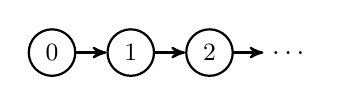
\begin{tikzpicture}[>=stealth', auto, semithick,
      flat/.style={circle,draw=black,thick,text=black,font=\small}]
      \node[flat]    at (0,0)  (base) {$0$};
      \node[flat]    at (1,0)  (n1) {$1$};
      \node[flat]    at (2,0)  (n2) {$2$};
      \node[flat,white]    at (3,0)  (n3) {$\ \ \  $};
      \node at (3,0) {$\ldots$};
      \draw[thick,->] (base) to (n1);
      \draw[thick,->] (n1) to (n2);
      \draw[thick,->] (n2) to (n3);
    \end{tikzpicture}
  \end{center}
  \noindent
  Here node $i$ represents the block broadcast by the leader of slot $i$
  and the arrows represent the direction of increasing time.
  %(Note that
  %the requirement of a single leader per slot is important in this
  %simple picture; it is possible for a network adversary to induce
  %divergent views between the players by taking advantage of slots where
  %more than a single honest participant is elected a leader.)

  \Paragraph{The blockchain axioms: Informal discussion.}
  The introduction of adversarial participants or multiple slot leaders
  complicates the family of possible blockchains that could emerge from
  this process. To explore this in the context of our protocols, we work
  with an abstract notion of a blockchain which
  % (as informally suggested above)
  ignores all internal structure. We consider a fixed assignment of
  leaders to time slots, and assume that the blockchain uses a proof
  mechanism to ensure that any block labeled with slot $\slot_t$ was
  indeed produced by a leader of slot $\slot_t$; this is guaranteed in
  practice by appropriate use of a secure digital signature scheme.

  Specifically, we treat a \emph{blockchain} as
  a sequence of abstract blocks, each labeled with a slot number, so
  that:
  \begin{enumerate}[label={\textbf{A\arabic*}}., ref={\textbf{A\arabic*}}, resume=axiom]
    \item\label{axiom:root} 
    The blockchain begins with a fixed ``genesis'' block, assigned to slot $\slot_0$.
    
    \item\label{axiom:labels} 
    The (slot) labels of the blocks are in strictly increasing order.
  \end{enumerate}
  It is further convenient to introduce the structure of a directed
  graph on our presentation, where each block is treated as a vertex; in
  light of the first two axioms above, a blockchain is a path beginning
  with a special ``genesis'' vertex, labeled $0$, followed by vertices
  with strictly increasing labels that indicate which slot is associated
  with the block. %(See the example below.)
  \begin{center}
    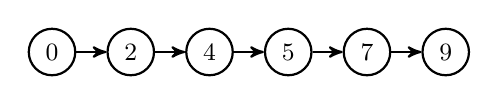
\begin{tikzpicture}[>=stealth', auto, semithick,
      flat/.style={circle,draw=black,thick,text=black,font=\small}]
      \node[flat]    at (0,0)  (base) {$0$};
      \node[flat]    at (1,0)  (n1) {$2$};
      \node[flat] at (2,0)  (n2) {$4$};
      \node[flat] at (3,0)  (n3) {$5$};
      \node[flat] at (4,0)  (n4) {$7$};
      \node[flat] at (5,0)  (n5) {$9$};
      \draw[thick,->] (base) to (n1);
      \draw[thick,->] (n1) to (n2);
      \draw[thick,->] (n2) to (n3);
      \draw[thick,->] (n3) -- (n4);
      \draw[thick,->] (n4) -- (n5);
    \end{tikzpicture}
  \end{center}
  The protocols of interest call for honest players to add a
  \emph{single} block %(to a single previous chain in its local state)
  during any slot. In particular:
  % \begin{enumerate}[label={\textbf{A\arabic*}}., resume=axiom]
  % \item If a slot $\slot_t$ was assigned to a single honest player, 
  % then a single block is created---during the entire protocol---with the label $\slot_t$.
  % \end{enumerate}
  \begin{enumerate}[label={\textbf{A\arabic*}}., ref={\textbf{A\arabic*}}, resume=axiom]
    \item\label{axiom:honest}
     Let $k \geq 1$ be an integer. 
    If a slot $\slot_t$ was assigned to $k$ honest players but no adversarial players, 
    then $k$ blocks are created---during the entire protocol---each having the label $\slot_t$.
  \end{enumerate}
  Recall that blockchains are \emph{immutable} in the sense that any
  block in the chain commits to the entire previous history of the
  chain; this is achieved in practice by including with each block a
  collision-free hash of the previous block. These properties imply that
  % if a specific slot $\slot_t$ was assigned to a unique honest player,
  % then any chain that includes the unique block from $\slot_t$ 
  % if a specific slot $\slot_t$ was assigned to a unique honest player,
  any chain that includes a block issued by an honest player 
  must also include that block's associated prefix in its entirety.

  As we analyze the dynamics of blockchain algorithms, it is convenient
  to maintain an entire family of blockchains at once. As a matter of
  bookkeeping, when two blockchains agree on a common prefix, we can
  glue together the associated paths to indicate this, as shown
  % in Figure~\ref{fig:glue-blockchains-into-fork}.
  below.

  % \begin{figure}[!htb]  
    \begin{center}
      \tikzsetnextfilename{glue-blockchains}
      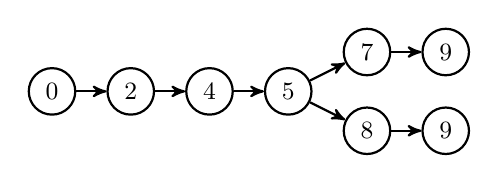
\begin{tikzpicture}[>=stealth', auto, semithick,
        flat/.style={circle,draw=black,thick,text=black,font=\small}]
        \node[flat]    at (0,0)  (base) {$0$};
        \node[flat]    at (1,0)  (n1) {$2$};
        \node[flat] at (2,0)  (n2) {$4$};
        \node[flat] at (3,0)  (n3) {$5$};
        \node[flat] at (4,.5)  (n4a) {$7$};
        \node[flat] at (5,.5)  (n5a) {$9$};
        \node[flat] at (4,-.5)  (n4b) {$8$};
        \node[flat] at (5,-.5)  (n5b) {$9$};
        \draw[thick,->] (base) to (n1);
        \draw[thick,->] (n1) to (n2);
        \draw[thick,->] (n2) to (n3);
        \draw[thick,->] (n3) to (n4a);
        \draw[thick,->] (n4a) to (n5a);
        \draw[thick,->] (n3) to (n4b);
        \draw[thick,->] (n4b) to (n5b);
      \end{tikzpicture}
      \end{center}
  %     \caption{A fork obtained by gluing together two blockchains.}
  %     \label{fig:glue-blockchains-into-fork}
  % \end{figure}
    When we glue together many chains to form such a diagram, we call it
    a ``fork''---the precise definition appears below. Observe that
    while these two blockchains agree through the vertex (block) labeled
    5, they contain (distinct) vertices labeled 9; this reflects two
    distinct blocks associated with slot 9 which, in light of the axiom
    above, 
    % must have been produced by an adversarial participant.
    may be produced by either an adversarial participant assigned to slot 9 or 
    two honest participants, both assigned to slot 9.
    
    Finally, as we assume that messages from honest players are
    delivered before the next slot begins, we note a direct consequence of the longest
    chain rule:
  \begin{enumerate}[label={\textbf{A\arabic*}}., ref={\textbf{A\arabic*}}, resume=axiom]
    \item\label{axiom:honest-depth} 
    If two honestly generated blocks $B_1$ and $B_2$ are labeled
    with slots $\slot_1$ and $\slot_2$ for which $\slot_1 < \slot_2$,
    then the length of the unique blockchain terminating at $B_1$ is
    strictly less than the length of the unique blockchain terminating at $B_2$.
  \end{enumerate}
  Recall that the honest participant(s) assigned to slot
  $\slot_2$ will be aware of the blockchain terminating at $B_1$ that
  was broadcast by an honest player in slot $\slot_1$ as a result of
  network synchrony; according to the longest-chain rule, 
  $B_2$ must have been placed on a chain that was at least this long. In contrast, not
  all participants are necessarily aware of all blocks generated by
  dishonest players, and indeed dishonest players may often want to
  delay the delivery of an adversarial block to a participant or show
  one block to some participants and show a completely different block
  to others.




\section{Characteristic strings and forks}\label{sec:char-string-mh}
Note that with the axioms we have discussed in Section~\ref{sec:pos-axioms}, 
whether or not a
particular fork diagram (such as the one 
% in Figure~\ref{fig:glue-blockchains-into-fork})
above) 
corresponds to a valid
execution of the protocol depends on how the slots have been awarded to the parties by the
leader election mechanism. We introduce the notion of a ``characteristic'' string as a convenient
means of representing information about slot leaders in a given execution.
% \begin{definition}[Characteristic string]
%   Let $\slot_1, \ldots, \slot_{n}$ be a sequence of slots. A \emph{characteristic string} $w$ is an element of $\{0,1\}^n$ defined for a particular execution of a blockchain protocol so that
%   \[
%     w_t =   \begin{cases}
%     0 & \text{if $\slot_{t}$ was assigned to a single honest participant},\\
% %    1 & \text{if $\slot_{t}$ was assigned to an adversarial participant},{}
%     1 & \text{otherwise.}
%   \end{cases}
% \]
% \end{definition}
\begin{definition}[Characteristic string]\label{def:trivalent-char-string}
  Let $\slot_1, \ldots, \slot_{n}$ be a sequence of slots.  A
  \emph{characteristic string} $w$ is an element of
  $\{\h,\H,\A\}^n$. The string $w$ is consistent with a particular
  execution of a blockchain protocol on these slots if for each
  $t \in [n]$, (i) if $w_t = \A$, the slot $\slot_t$ is assigned to
  at least one adversarial participant, (ii) if $w_t = \h$, the slot
  $\slot_{t}$ is assigned to a unique, honest participant, and (iii)
  if $w_t = \H$, the slot $\slot_{t}$ is assigned to at least one
  honest participant and no adversarial participants.

  Observe that when an execution corresponds to a characteristic
  string $w$, it also corresponds to any string obtained from $w$ by
  replacing $\h$ symbols with $\H$ symbols.
% 
  % \[
  %   w_t =   \begin{cases}
  %   \h & \text{if $\slot_{t}$ was assigned to a single participant who is honest},\\
  %   \H & \text{if $\slot_{t}$ was assigned to two or more participants, all honest},\\
  %   \A & \text{otherwise.}
  %   \end{cases}
  % \]
\end{definition}
For two strings $x$ and $w$ on the same alphabet, 
we write $x \Prefix w$ if and only if $x$ is a strict prefix of $w$. 
Similarly, 
we write $x \PrefixEq w$ if and only if either $x = w$ or $x \Prefix w$. 
The empty string $\varepsilon$ is a prefix to any string. 
If $w_t \in \{\h, \H\}$, we say that ``$\Slot_t$ is honest'' and 
otherwise, we say that ``$\Slot_t$ is adversarial.'' 
With this discussion behind us, we set down the formal object we use
to reflect the various blockchains adopted by honest players during
the execution of a blockchain protocol. This definition formalizes the blockchains axioms discussed above.

%%%%Forks

\begin{definition}[Fork]\label{def:fork}
  Let $w\in \{\h, \H, \A\}^n$, $P = \{ i : w_i = \h\}$, and $Q = \{ j : w_j = \H\}$. 
  A \emph{fork} for the string $w$ consists of a directed and rooted
  tree $F=(V,E)$ with a labeling $\ell:V\to\{0,1,\dots,n\}$. We insist
  that each edge of $F$ is directed away from the root vertex and
  further require that
  \begin{enumerate}[label=(F{\arabic*})]
    \item\label{fork:root-mh} the root vertex $r$ has label $\ell(r)=0$;

    \item\label{fork:monotone-mh} the labels of vertices along any directed path are strictly increasing;

    \item\label{fork:unique-honest-mh}\label{fork:multiply-honest}
    each index $i\in P$ 
    is the label of exactly one vertex of $F$ 
    and 
    % \item
    each index $j\in Q$ 
    is the label of at least one vertex of $F$; and 

    \item\label{fork:honest-depth-mh} 
    for any indices $i,j\in P \Union Q$, 
    if $i<j$ then 
    the depth of a vertex with label $i$ 
    is strictly less than 
    the depth of a vertex with label $j$.
  \end{enumerate}
\end{definition}

If $F$ is a fork for the characteristic string $w$, we write
$F\vdash w$.  The conditions~\ref{fork:root-mh}--\ref{fork:honest-depth-mh}
are analogues of the axioms~\ref{axiom:root}--\ref{axiom:honest-depth}
above. The formal reflection of axiom~\ref{axiom:honest} by
condition~\ref{fork:multiply-honest} deserves further comment: We have
chosen a definition of characteristic string that does not indicate
the number of honest victories in cases where there may be many; in
particular, the symbol $\H$ may be associated with any positive number
of (honest) vertices in the fork. Indeed, we even permit a fork to
have a \emph{single} honest vertex associated with such a symbol,
which enlarges the class of forks under consideration for a particular
characteristic string. This strengthens our results by effectively
giving the adversary the option to treat $\H$ symbols as $\h$
symbols. See Fig.~\ref{fig:fork-mh}
% in Section~\ref{sec:figures} 
for an example fork. 

\begin{figure}[t]
  \centering
  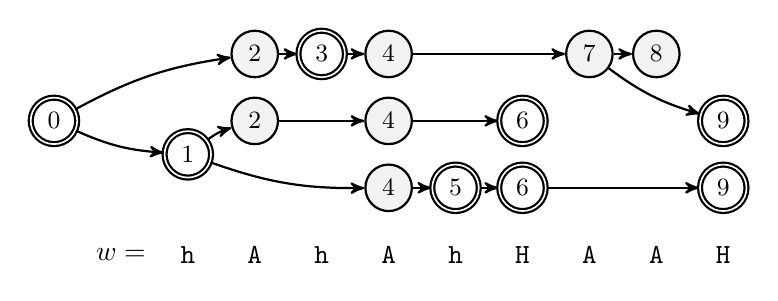
\begin{tikzpicture}[scale=0.85,>=stealth', auto, semithick,
    honest/.style={circle,draw=black,thick,text=black,double,font=\small},
    malicious/.style={fill=gray!10,circle,draw=black,thick,text=black,font=\small}]
    \node at (0,-2) {$w =$};
    \node at (1,-2) {$\h$};
    \node[honest]    at (1,-.5)  (ab1) {$1$};
    \node at (2,-2) {$\A$};
    \node[malicious] at (2,0)  (b2) {$2$}; \node[malicious] at (2,1) (c1) {$2$};
    \node at (3,-2) {$\h$};    \node[honest]    at (3,1)  (c2) {$3$};
    \node at (4,-2) {$\A$};    \node[malicious] at (4,0)  (b3) {$4$}; \node[malicious] at (4,-1) (a2) {$4$};
    \node[malicious] at (4,1) (c3) {$4$};
    \node at (5,-2) {$\h$};    \node[honest]    at (5,-1) (a3) {$5$};
    \node at (6,-2) {$\H$};    \node[honest]    at (6,0)  (b4) {$6$}; \node[honest]    at (6,-1)  (a4) {$6$};
    \node at (7,-2) {$\A$};    \node[malicious] at (7,1)  (c4) {$7$};
    \node at (8,-2) {$\A$};    \node[malicious] at (8,1)  (c5) {$8$};
    \node at (9,-2) {$\H$};    \node[honest]    at (9,0)  (b5) {$9$}; \node[honest]    at (9,-1)  (a5) {$9$};
    \node[honest] at (-1,0) (base) {$0$};
    % \node[state,honest] at (3,-1) (bottom) {};
    % \node[state,honest] at (7,1) (top) {$H$};
    \draw[thick,->] (base) to[bend left=10] (c1);
    \draw[thick,->] (base) to[bend right=10] (ab1);
    \draw[thick,->] (ab1) to[bend right=10] (a2);
    \draw[thick,->] (a2) -- (a3);
    \draw[thick,->] (a3) -- (a4);
    \draw[thick,->] (ab1) to[bend left=10] (b2);
    \draw[thick,->] (b2) -- (b3);
    \draw[thick,->] (b3) -- (b4);
      % \draw[thick,->] (b4) -- (b5);
    \draw[thick,->] (c4) to[bend right=10] (b5);
    \draw[thick,->] (a4) -- (a5);
    \draw[thick,->] (c1) -- (c2);
    \draw[thick,->] (c2) -- (c3);
    \draw[thick,->] (c3) -- (c4);
    \draw[thick,->] (c4) -- (c5);
    % \draw[thick,<->] (3,0) -- (7,0) node[pos=.5] {$\gap(f)$};
  \end{tikzpicture}
  \caption{A fork $F$ for the characteristic string $w = \h\A\h\A\h\H\A\A\H$;
    vertices appear with their labels and honest vertices are
    highlighted with double borders. Note that the depths of the
    (honest) vertices associated with the honest indices of $w$ are
    strictly increasing. Note, also, that this fork has three disjoint
    paths of maximum depth. 
    In addition, two honest vertices have label 6 and two more have label 9, 
    indicating the fact that two honest leaders are associated with each of the (honest) slots 6 and 9. 
    Honest vertices with the same label are concurrent and, therefore, cannot extend each other.
    Note that the two honest vertices with label 6 extend different vertices with the same depth. 
    This is allowed since any tie in the longest-chain rule is broken by the adversary. 
    }
  \label{fig:fork}
\end{figure}


A final notational convention: If $F \vdash x$ and
$\hat{F} \vdash w$, we say that $F$ is a \emph{prefix} of $\hat{F}$,
written $F \fprefix \hat{F}$, if 
% the string $x \in \{0,1\}^\ell$ is a prefix of the string $w \in \{0,1\}^{\ell + m}$ 
$x \PrefixEq w$
and $F$ appears as a
consistently-labeled subgraph of $\hat{F}$. 
(Specifically, each path of $F$ appears, with identical labels, in $\hat{F}$.) 


% Observe that any string of the form $0^k$ has a unique
% fork consisting of a single path:
% \begin{center}
%   \begin{tikzpicture}[scale=1,>=stealth', auto, semithick,
%     flat/.style={circle,draw=black,thick,text=black,font=\small}]
%     \node[flat] at (0,0)  (base) {$0$};
%     \node[flat] at (1,0)  (n1) {$1$};
%     \node[flat] at (2,0)  (n2) {$2$};
%     \node[flat] at (5,0)  (n5) {$k$};
%     \draw[thick,->] (base) to (n1);
%     \draw[thick,->] (n1) to (n2);
%     \draw[thick,->,dashed] (n2) to (n5);
%   \end{tikzpicture}
% \end{center}
% On the other hand, there are in fact an infinite number of forks for
% any string with at least one ``1,'' as slots for which $w_i = 1$ can
% be associated with any number of vertices. Axiom~\ref{fork:monotone-mh}
% reflects that any legal chain must consist of blocks with increasing
% slot labels. Axiom~\ref{fork:unique-honest} reflects the fact that honest plays produce a single block. Axiom~\ref{fork:honest-depth} reflects that each new
% honest vertex is always placed at a depth strictly greater than all
% previous honest vertices, because honest users always choose to add
% their block to the longest visible chain, and we assume honest blocks
% can be seen by all users. (By contrast, adversaries may play on
% shorter tines, or may ``hide'' dishonest blocks from other users until
% later slots.)



  Let $w$ be a characteristic string.  The directed paths in the fork
  $F \Fork w$ originating from the root are called \emph{tines}; these
  are abstract representations of blockchains. (Note that a tine may 
  not terminate at a leaf of the fork.)  We naturally extend the label
  function $\ell$ for tines: i.e., $\ell(t) \triangleq \ell(v)$ where
  the tine $t$ terminates at vertex $v$. The length of a tine $t$ is
  denoted by $\length(t)$.

 \Paragraph{Viable tines.}
 The longest-chain rule dictates that honest players build on chains
 that are at least as long as all previously broadcast honest
 chains. It is convenient to distinguish such tines in the analysis:
 specifically, a tine $t$ of $F$ is called \emph{viable} if its length
 is no smaller than the depth of any honest vertex $v$ for which
 $\ell(v) \leq \ell(t)$. A tine $t$ is \emph{viable at slot $s$} if
 the length of the portion of $t$ appearing over slots $0,\ldots, s$ 
 is no smaller than the depths of any honest vertices labeled from these slots. (As noted,
 the properties~\ref{fork:multiply-honest} and~\ref{fork:honest-depth-mh}
 together imply that an honest observer at slot $s$ will only adopt a
 viable tine.)  
 % The \emph{honest depth} function
 % $\hdepth : H \rightarrow [n]$ gives the depth of the (unique) vertex
 % associated with an honest slot; by~\ref{fork:honest-depth},
 % $\hdepth(\cdot)$ is strictly increasing.
 The \emph{honest depth} function
 $\hdepth : P \Union Q \rightarrow [n]$, 
 defined as $\hdepth(i) = \max_{t \in F} \left\{ \length(t) \SuchThat \ell(t) = i \right\}$, 
 gives the largest depth of the (honest) vertices 
 associated with an honest slot; by~\ref{fork:honest-depth-mh},
 $\hdepth(\cdot)$ is strictly increasing.


% \subsection{Comments on the model}\label{sec:model-comments}





    % \begin{definition}[Conservative fork]\label{def:conservative-fork}
    %   The term \emph{conservative fork} is defined inductively, as follows.
    %   The trivial fork $F_0$ for the empty string $\varepsilon$ 
    %   is conservative. 
    %   A fork $F_{T} \Fork w0$ is conservative if 
    %   the fork prefix $F_{T_1} \ForkPrefix F_T, F_{T-1} \Fork w$ 
    %   is conservative 
    %   and every honest tine $t \in F_T$ at slot $T$ 
    %   is a conservative extension with respect to $F_{T-1}$.
    %   Likewise, 
    %   a fork $F_{T} \Fork w1$ is conservative if 
    %   the fork prefix $F_{T_1} \ForkPrefix F_T, F_{T-1} \Fork w$ 
    %   is conservative and $F_T = F_{T-1}$. 
    % \end{definition}
    % Observe that a conservative fork is closed. 

    % We record the following lemma from [LinearConsistencyPaper].
    % \begin{lemma}[Optimal online adversary]\label{lemma:online-adversary}
    %   For every characteristic string $w = xy$ 
    %   there is a closed fork $F \Fork xy$ 
    %   so that 
    %   $\reach(F) = \reach(xy)$ and $\mu_x(F) = \mu_x(y)$. 
    % \end{lemma}
    % % Given a charactersistic string $w = xy$, 
    % % the ``online adversary'' given in the LinearConsistencyPaper 
    % % creates a conservative fork 
    % % which achieves the reach and relative margin of the string $xy$. 


\section[Slot Settlement and UVP]{Slot settlement and the Unique Vertex Property (UVP)}\label{sec:model-settlement}
  
  We are now ready to explore the power of an adversary in this
  setting who has corrupted a (perhaps evolving) coalition of the
  players. We focus on the possibility that such an adversary can
  violate the consistency of the honest players'
  blockchains. In particular, we consider the possibility that, at
  some time $t$, the adversary conspires to produce two maximum-length blockchains 
  that diverge prior to a previous slot $s \leq t$; in
  this case honest players adopting the longest-chain rule may clearly
  disagree about the history of the blockchain after slot $s$. We call
  such a circumstance a \emph{settlement violation}.

  To express this in our abstract language, let $F \Fork w$ be a fork
  corresponding to an execution with characteristic string $w$. Such a
  settlement violation induces two viable tines $t_1, t_2$ with the
  same length that diverge prior to a particular slot of interest. We
  record this below.
    
  \begin{definition}[Settlement with parameters $s,k \in \NN$]\label{def:settlement-mh}
    Let $n \in \NN$ and let $w$ be a characteristic string of length $n$. 
    Let $t \in [s + k, n]$ be an integer, $\hat{w} \PrefixEq w, |\hat{w}| = t$, and 
    let $F$ be any fork for $\hat{w}$. 
    We say that a slot $s$ is \emph{not $k$-settled} in $F$ if 
    $F$ contains two maximum-length tines $\Chain_1, \Chain_2$ 
    that ``diverge prior to $s$,'' i.e., they either
    contain different vertices labeled with $s$, or one contains a
    vertex labeled with $s$ while the other does not. 
    Otherwise, we say that \emph{slot $s$ is $k$-settled in $F$}. 
    We say that \emph{slot $s$ is $k$-settled in $w$} if, 
    for each $t \geq s+k$, 
    it is $k$-settled in every fork $F \Fork \hat{w}$ where $\hat{w} \PrefixEq w, |\hat{w}| = t$.
  \end{definition}




  \begin{figure*}[t]
    \singlespacing
    \begin{center}
      \fbox{
        \begin{minipage}{\textwidth}
          \begin{center}
            \textbf{The $(\Distribution,T;s,k)$-settlement game}
          \end{center}
          \begin{enumerate}

          \item A characteristic string $w \in \{\h,\H,\A\}^T$ is drawn from
            $\mathcal{D}$. (This reflects the results of the leader
            election mechanism.)

          \item Let $A_0 \vdash \varepsilon$ denote the initial fork for
            the empty string $\varepsilon$ consisting of a single node
            corresponding to the genesis block.

          \item For each slot $\Slot_t, t = 1, \ldots, T$ in increasing order:
            \begin{enumerate}
            \item\label{game:honest} (Honest slot.)  This case
              pertains to $w_t \in \{\h, \H\}$.  If $w_t = \h$ then
              $\Adversary$ sets $k = 1$.  If $w_t = \H$ then
              $\Adversary$ chooses an arbitrary integer $k \geq 1$.
              The challenger is then given $k$ and the fork
              $A_{t-1} \vdash w_1 \ldots w_{t-1}$.  He must determine
              a new fork $F_{t} \vdash w_1 \ldots w_t$ by adding $k$
              new vertices (all labeled with $t$) to $A_{t-1}$.  Each
              new vertex is added at the end of a maximum-length path
              in $A_{t-1}$.  If there are multiple
              candidates\footnote{ It is possible that all maximum-length 
                tines are honest. In the settlement game
                considered in~\cite{LinearConsistencySODA}, at least
                one of these tines was adversarial.} 
              for this path,
              $\Adversary$ may break the tie.  If $k \geq 2$, multiple
              vertices (all with label $t$) may be added at the end of
              the same path.



            \item 
            (Adversarial slot.)
            If $w_t = \A$, this is an adversarial slot. $\Adversary$
              may set $F_t \vdash w_1\ldots w_t$ to be an arbitrary fork
              for which $A_{t-1} \fprefix F_t$.
              
            \item (Adversarial augmentation.) $\Adversary$ determines an
              arbitrary fork $A_t \vdash w_1 \ldots, w_{t}$ for
              which $F_{t} \fprefix A_{t}$.
            \end{enumerate}
             Recall that $F \fprefix F'$ indicates that $F'$
              contains, as a consistently-labeled subgraph, the fork $F$.
          \end{enumerate}
          $\Adversary$ \emph{wins the settlement game} if slot $s$ is not
          $k$-settled in some fork $A_t, t \geq s+k$.
        \end{minipage}
      }
    \end{center}
  \end{figure*}



  \begin{definition}[Bottleneck Property (BP) and Unique Vertex Property (UVP)]\label{def:bottleneck-property}\label{def:unique-vertex-property}
    Let $w \in \{\h, \H, \A\}^T$ be a characteristic string.  
    A slot $s \in [T]$ is said to have the 
    \emph{bottleneck property in $w$} 
    if, 
    for any fork $F \Fork w$ 
    and any $k \geq s + 1$, 
    every tine viable at the onset of slot $k$ 
    contains, as its prefix, some vertex with label $s$.       
    Slot $s$ is said to have the \emph{Unique Vertex Property} 
    if, 
    for any fork $F \Fork w$, 
    there is a unique vertex $u \in F$ with label $s$ 
    so that 
    for any $k \geq s + 1$, 
    all tines viable at the onset of slot $k$ 
    contain, as their common prefix, 
    the vertex $u$.
  \end{definition}
  Thus 
  if a uniquely honest slot in $w$ has the bottleneck property, 
  it has the UVP as well.
  As a consistency property, UVP has several advantages over slot settlement. 
  First, it easily implies the slot settlement property:
  let $w \in \{\h, \H, \A\}^T, s \in [T]$, and $k \in [T - s]$. 
  \begin{equation}\label{eq:settlement-uvp}
    \text{If a slot $t \in [s, s + k]$ has UVP in $w$ 
    then $s$ is $k$-settled in $w$.}     
  \end{equation}  
  In addition, UVP has a straightforward characterization 
  using ``Catalan slots'' 
  (see Theorem~\ref{thm:unique-honest}) 
  and ``relative margin'' 
  (see Lemma~\ref{lemma:uvp-margin}); 
  these characterizations are amenable to stochastic analysis. 
  Finally, since UVP is structurally reminiscent of the traditional common prefix (CP) violations, 
  % (see Section~\ref{sec:cp-model}), 
  UVP easily implies CP. 
  The analogous statement ``settlement implies CP,'' however, 
  requires a lengthy proof both in~\cite{LinearConsistency} and in 
  our framework. See 
  \Section~\ref{sec:cp-multihonest}
  % the full version~\cite{MultiHonestFullVersion}
  for details.




\section[Attacks on Settlement]{Adversarial attacks on settlement time; the settlement game}\label{sec:game-mh} 


  To clarify the relationship between forks and the chains at play in a
  canonical blockchain protocol, we define a game-based model below that
  explicitly describes the relationship between forks and executions.
  By design, the probability that the adversary wins this game is at
  most the probability that a slot $s$ is not $k$-settled. 
  % We remark
  % that while we focus on settlement violations for clarity, one could
  % equally well have designed the game around common prefix violations.

  Consider the \emph{$(\Distribution,T;s,k)$-settlement game} 
  (presented in the box), played
  between an adversary $\Adversary$ and a challenger $\Challenger$ with
  a leader election mechanism modeled by an ideal distribution
  $\Distribution$. Intuitively, the game should reflect the ability of
  the adversary to achieve a settlement violation; that is, to present
  two maximum-length viable blockchains to a future honest observer,
  thus forcing them to choose between two alternate histories which
  disagree on slot $s$.
  The challenger plays the role(s) of the honest players during the
  protocol. 

  It is important to note that the game bestows the player $\Adversary$ 
  with the power to choose the number of honest vertices in 
  a multihonest slot. 
  Note that this setting makes the player strictly more powerful and, 
  importantly, implies that 
  the game is completely determined 
  by the choices made by $\Adversary$ 
  (i.e., the actions of the challenger are deterministic). 
  Consequently, in Definition~\ref{def:settlement-mh-insecurity}, 
  we can use a single, implicit universal quantifier 
  over all strategies $\Adversary$; no choices of the challenger are actually necessary to fully describe the game.


  \begin{definition}[Settlement insecurity]\label{def:settlement-mh-insecurity}
    Let $\Distribution$ be a distribution on $\{\h, \H, \A\}^T$. 
    Let $w \sim \Distribution$ be the string used in the 
    first step of a $(\Distribution, T; s, k)$-settlement game $G$. 
    The \emph{$(s,k)$-settlement insecurity} of $\Distribution$ 
    is defined as 
    \[
      \mathbf{S}^{s,k}[\Distribution] \triangleq 
        \max_{\substack{\hat{w} \PrefixEq w \\ |\hat{w}| \geq s + k}}\,
        \max_{F \Fork \hat{w}}\, 
        \Pr\left[\parbox{50mm}{\centering $F$ has two maximum-length tines that diverge prior to slot $s$}\right]
      \,.
    \]
    % this maximum taken over all adversaries $\Adversary$.
    Note that the probability in the right-hand side is the same as 
    the probability that $\Adversary$ wins $G$.
  \end{definition}

  \section{Main theorem for PoS consistency in the synchronous setting}\label{sec:main-thm-multihonest}
  Note that in typical PoS settings the distribution $\Distribution$
  is determined by the combined stake held by the adversarial players,
  the leader election mechanism, and the dynamics of the protocol. The
  most common case (as seen in Snow White~\cite{SnowWhite},
  Ouroboros~\cite{Ouroboros}, and Ouroboros Praos~\cite{Praos})
  guarantees that the characteristic string $w = w_1 \ldots w_T$ is
  drawn from an i.i.d.\ distribution for which
  $\Pr[w_i = \A] \leq (1 - \epsilon)/2$ for some $\epsilon \in (0, 1)$;
  here the constant $(1-\epsilon)/2$ is directly related to the stake
  held by the adversary. Some settings involving adaptive adversaries
  (e.g., Ouroboros Praos~\cite{Praos}) yield a weaker martingale-type
  guarantee that
  $\Pr[w_i = \A \mid w_1, \ldots, w_{i-1}] \leq (1 - \epsilon)/2$.  We
  can easily handle both types of distributions in our analysis since
  the former distribution ``stochastically dominates'' the latter; 
  see Section~\ref{sec:martingale-dominance} for a precise definition.
  % Let us define below the notion of stochastic dominance. 
  As a rule, we denote the
  probability distribution associated with a random variable using
  uppercase script letters. 
  \begin{definition}[Stochastic dominance]\label{def:dominance-mh} 
    Let $X$ and $Y$ be random variables taking values in some set $\Omega$ 
    endowed with a partial order $\leq$. 
    We say that $X$ \emph{stochastically dominates} $Y$, 
    written $Y \dominatedby X$, if 
    $
      \mathcal{X}(A) \geq \mathcal{Y}(A)
      % \,.
    $ 
    for all \emph{monotone sets} $A \subseteq \Omega$, 
    where a set $A \subseteq \Omega$ is called 
    monotone if $a \in A$ implies $a' \in A$ for all $a \leq a'$.
    As a special case, when $\Omega = \R$,  $Y \dominatedby X$ if
    $\Pr[X \geq \Lambda] \geq \Pr[Y \geq \Lambda]$
    for every $\Lambda \in \R$.  
    We extend this notion to probability
    distributions in the natural way.
  \end{definition}

  Throughout the paper, we adopt the following partial order on
  $\{\h, \H, \A\}^T$: If $T = 1$, define $\h < \H < \A$.  Otherwise,
  for two strings $xa, yb \in \{\h, \H, \A\}^T, |a| = |b| = 1$,
  $xa \leq yb$ if and only if $x \leq y$ and $a \leq b$. When
  $x \leq y$, one might say that $y$ is ``more adversarial'' than $x$:
  indeed, if $F \vdash x$ and $x \leq y$ then $F \vdash y$ so that any
  settlement violation for $x$ induces a settlement violation for $y$.

  \begin{definition}[$(\epsilon, p_\h)$-Bernoulli
    condition]\label{def:bernoulli-cond}
    Let $T \in \NN, \epsilon \in (0,1)$, and
    $p_\h \in [0,(1+\epsilon)/2]$. Define $p_\A = (1-\epsilon)/2$ and
    $p_\H = 1- p_\A - p_\h$.  A random variable $w = w_1 \ldots w_T$
    taking values in $\{\h, \H, \A\}^T$ is said to satisfy the
    \emph{$(\epsilon, p_\h)$-Bernoulli condition} if each
    $w_i, i \in [T]$, is independent and identically distributed as
    follows: $\Pr[w_i = \sigma] = p_\sigma$ for
    $\sigma \in \{\h, \H, \A\}$.  The distribution of $w$ is also said
    to satisfy the $(\epsilon, p_\h)$-Bernoulli condition.

    We frequently use the notation $p_\H$ and $p_\A$ in the context of
    such a random variable when $\epsilon$ and $p_\h$ can be inferred
    from context.
  \end{definition}
  
  \begin{theorem}[Main theorem]\label{thm:main-mh}
    Let $\epsilon, p_\h \in (0, 1)$ and $s, k, T \in \NN$.  
    Let $\mathcal{B}$ be a distribution 
    on length-$T$ characteristic strings satisfying 
    the $(\epsilon, p_\h)$-Bernoulli condition.
    Then 
    $
      \mathbf{S}^{s,k}[\mathcal{B}] 
        \leq 
        \exp\left(-k\cdot \Omega( 
          \min(\epsilon^3, \epsilon^2 p_\h) 
        \right)
        % \,.
    $.
    Furthermore, 
    let 
    $\mathcal{W}$ be a distribution on
    $\{\h, \H, \A\}^T$ so that 
    $\mathcal{W} \DominatedBy \mathcal{B}$. 
    Then $\mathbf{S}^{s,k}[\mathcal{W}] 
        \leq \mathbf{S}^{s,k}[\mathcal{B}]$.   
    (Here, the asymptotic notation hides constants that do not depend on $\epsilon$ or $k$.)
  \end{theorem}
  Note that the quantity $p_\h$ above cannot be zero.
  We present the proof in \Section~\ref{sec:bounds-main-proofs-multihonest}. 
  In \Section~\ref{sec:fork-framework}, 
  we give a characterization of the UVP which 
  allows us to explicitly compute $\mathbf{S}^{s,k}[\mathcal{B}]$; 
  see 
  % Lemma~\ref{lemma:uvp-margin}, 
  Theorem~\ref{thm:relative-margin} and 
  \Section~\ref{sec:exact-prob-multihonest}.


  \Paragraph{Analysis in the $\Delta$-synchronous setting.} The security
   game above most naturally models a blockchain protocol over a
   synchronous network with immediate delivery (because each ``honest''
   play of the challenger always builds on a fork that contains the fork
   generated by previous honest plays). However, the model can be easily
   adapted to protocols in the $\Delta$-synchronous model by applying
   the $\Delta$-reduction mapping of~\cite{Praos} (which is specifically
   designed to lift the synchronous analysis to the $\Delta$-synchronous
   setting).
   These details appear in \Section~\ref{sec:async-multihonest}.


  \Paragraph{Public leader schedules.} One attractive feature of this
  model is that it gives the adversary full information about the future
  schedule of leaders. The analysis of some protocols indeed demand this
  (e.g., Ouroboros, Snow White). Other protocols---especially those
  designed to offer security against adaptive adversaries (Praos,
  Genesis)---in fact contrive to keep the leader schedule private. Of
  course, as our analysis is in the more difficult ``full information''
  model, it applies to all of these systems.

  \Paragraph{Bootstrapping multi-phase algorithms; stake shift.} We remark that
  several existing proof-of-stake blockchain protocols proceed in
  phases, each of which is obligated to generate the randomness (for
  leader election, say) for the next phase based on the current stake
  distribution. The blockchain security properties of each phase are
  then individually analyzed---assuming clean randomness---which yields
  a recursive security argument; in this context the game outlined above
  precisely reflects the single phase analysis.






%%% Local Variables:
%%% mode: latex
%%% TeX-master: "main"
%%% End:


\section{Unique Vertex Property via Catalan slots}\label{sec:definitions}
We rely on the elementary framework of forks and margin
from~\citet{KRDO17}. We restate and briefly discuss the pertinent
definitions below. With these basic notions behind us, we then define
a new ``relative'' notion of margin, which will allow us to
significantly improve the efficacy of these tools for reasoning about
settlement times.
%In particular, these tools will allow us to reason
%about the possibility that an adversary can produce two alternate
%histories of the blockchain that diverge prior to a particular block.

Recall that for a given execution of the protocol, we record the
result of the leader election process via a \emph{characteristic
  string} $w \in \{0,1\}^T$, defined such that $w_i = 0$ when a unique
and honest party is assigned to slot $i$ and $w_i = 1$ otherwise.
A vertex of a fork is said to be \emph{honest}
  if it is labeled with an index $i$ such that $w_i=0$.

\begin{definition}[Tines, length, and height]
  Let $F \vdash w$ be a fork for a characteristic string.  A
  \emph{tine} of $F$ is a directed path starting from the root. For
  any tine $t$ we define its \emph{length} to be the number of edges
  in the path, and for any vertex $v$ we define its \emph{depth} to be
  the length of the unique tine that ends at $v$. 
  If a tine $t_1$ is a strict prefix of another tine $t_2$, we write $t_1 \Prefix t_2$. 
  Similarly, if $t_1$ is a non-strict prefix of $t_2$, we write $t_1 \PrefixEq t_2$.
  The longest common prefix of two tines $t_1, t_2$ is denoted by $t_1 \Intersect t_2$. 
  That is, $\ell(t_1 \Intersect t_2) = \max\{\ell(u) \SuchThat \text{$u \PrefixEq t_1$ and $u \PrefixEq t_2$} \}$. 
  The \emph{height} of
  a fork (as usual for a tree) is the length of the longest tine,
  denoted $\height(F)$. 
\end{definition}

\begin{definition}[The $\sim_x$ relations]
  For two tines $t_1$ and $t_2$ of a fork $F$, we write $t_1 \sim t_2$
  when $t_1$ and $t_2$ share an edge; otherwise we write
  $t_1 \nsim t_2$. We generalize this equivalence relation to reflect
  whether tines share an edge over a particular suffix of $w$: for
  $w = xy$ we define $t_1 \sim_x t_2$ if $t_1$ and $t_2$ share an edge
  that terminates at some node labeled with an index in $y$;
  otherwise, we write $t_1 \nsim_x t_2$ (observe that in this case the
  paths share no vertex labeled by a slot associated with $y$).  We
  sometimes call such pairs of tines \emph{disjoint} (or, if
  $t_1 \nsim_x t_2$ for a string $w = xy$, \emph{disjoint over
    $y$}). Note that $\sim$ and $\sim_\varepsilon$ are the same
  relation.
\end{definition}

%Informally, $t_1\sim_x t_2$ indicates that when we restrict our view of history to only blocks \emph{after}
%the prefix $x$, $t_1$ and $t_2$ share an edge (and thus agree on at least one block after that point).

The basic structure we use to use to reason about settlement times is
that of a ``balanced fork.''

\begin{definition}[Balanced fork; cf.\ ``flat'' in \cite{KRDO17}]\label{def:balanced-fork} A
  fork $F$ is \emph{balanced} if it contains a pair of tines $t_1$ and
  $t_2$ for which $t_1\nsim t_2$ and
  $\length(t_1)=\length(t_2)=\height(F)$. We define a relative notion
  of balance as follows: a fork $F \vdash xy$ is \emph{$x$-balanced}
  if it contains a pair of tines $t_1$ and $t_2$ for which
  $t_1 \not\sim_x t_2$ and $\length(t_1) = \length(t_2) = \height(F)$.
\end{definition}

Thus, balanced forks contain two completely disjoint, maximum-length
tines, while $x$-balanced forks contain two maximum-length tines that
may share edges in $x$ but must be disjoint over the rest of the
string. 
See Figures~\ref{fig:balanced} and~\ref{fig:x-balanced} 
for examples of balanced forks.
\begin{figure}[ht]
  \centering
  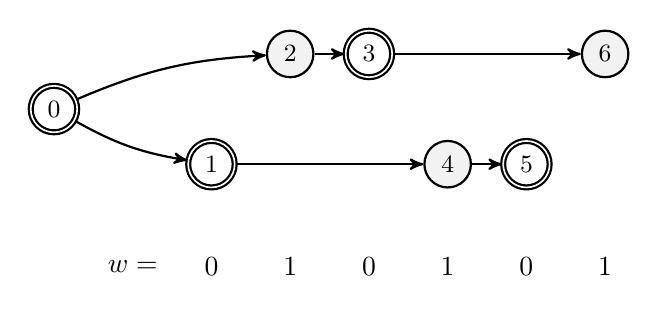
\begin{tikzpicture}[>=stealth', auto, semithick,
    honest/.style={circle,draw=black,thick,text=black,double,font=\small},
   malicious/.style={fill=gray!10,circle,draw=black,thick,text=black,font=\small}]
    \node at (0,-2) {$w =$};
  \node at (1,-2) {$0$}; \node[honest] at (1,-.7) (b1) {$1$};
  \node at (2,-2) {$1$}; \node[malicious] at (2,.7) (a1) {$2$};
  \node at (3,-2) {$0$}; \node[honest] at (3,.7) (a2) {$3$};
  \node at (4,-2) {$1$}; \node[malicious] at (4,-.7) (b2) {$4$};
  \node at (5,-2) {$0$}; \node[honest] at (5,-.7) (b3) {$5$};
  \node at (6,-2) {$1$}; \node[malicious] at (6,.7) (a3) {$6$};
    \node[honest] at (-1,0) (base) {$0$};
  \draw[thick,->] (base) to[bend left=10] (a1);
      \draw[thick,->] (a1) -- (a2);
      \draw[thick,->] (a2) -- (a3);
  \draw[thick,->] (base) to[bend right=10] (b1);
      \draw[thick,->] (b1) -- (b2);
      \draw[thick,->] (b2) -- (b3);
    \end{tikzpicture} 
  \caption{A balanced fork}
  \label{fig:balanced}
\end{figure}

\begin{figure}[ht]
  \centering
  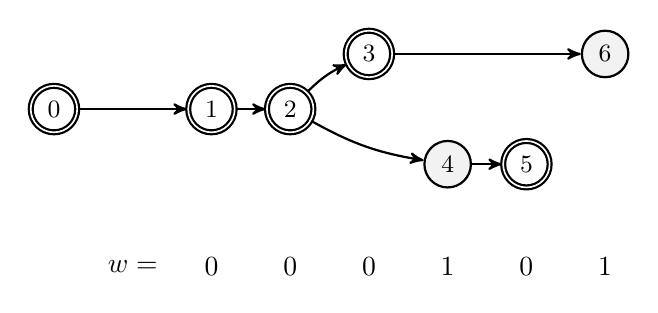
\begin{tikzpicture}[>=stealth', auto, semithick,
    honest/.style={circle,draw=black,thick,text=black,double,font=\small},
   malicious/.style={fill=gray!10,circle,draw=black,thick,text=black,font=\small}]
    \node at (0,-2) {$w =$};
  \node at (1,-2) {$0$}; \node[honest] at (1,0) (ab1) {$1$};
  \node at (2,-2) {$0$}; \node[honest] at (2,0) (ab2) {$2$};
  \node at (3,-2) {$0$}; \node[honest] at (3,.7) (a3) {$3$};
  \node at (4,-2) {$1$}; \node[malicious] at (4,-.7) (b3) {$4$};
  \node at (5,-2) {$0$}; \node[honest] at (5,-.7) (b4) {$5$};
  \node at (6,-2) {$1$}; \node[malicious] at (6,.7) (a4) {$6$};
    \node[honest] at (-1,0) (base) {$0$};
  \draw[thick,->] (base) -- (ab1);
  \draw[thick,->] (ab1) -- (ab2);
  \draw[thick,->] (ab2) to[bend left=10] (a3);
    \draw[thick,->] (a3) -- (a4);
  \draw[thick,->] (ab2) to[bend right=10] (b3);
    \draw[thick,->] (b3) -- (b4);
    \end{tikzpicture} 
  \caption{An $x$-balanced fork, where $x=00$}
  \label{fig:x-balanced}
\end{figure}


\Paragraph{Balanced forks and settlement time.}
A fundamental question arising in typical blockchain settings is how
to determine \emph{settlement time}, the delay after which the
contents of a particular block of a blockchain can be considered
stable. The existence of a balanced fork is a precise indicator for
``settlement violations'' in this sense. Specifically, consider a
characteristic string $xy$ and a transaction appearing in a block
associated with the first slot of $y$ (that is, slot $|x| + 1$). One
clear violation of settlement at this point of the execution is the
existence of two chains---each of maximum length---which diverge
\emph{prior to $y$}; in particular, this indicates that there is an
$x$-balanced fork $F$ for $xy$. Let us record this observation below.

\begin{observation}\label{obs:settlement-balanced-fork}
  Let $s, k \in \NN$ be given and 
  let $w$ be a characteristic string. 
  Slot $s$ is not $k$-settled for the characteristic string $w$ 
  if 
  there exist a decomposition $w = xyz$, 
  where $|x| = s - 1$ and $|y| \geq k+1$, 
  and an $x$-balanced fork for $xy$. 
\end{observation}

In fact, every $\kSlotCP$ violation produces a balanced fork as well;
see Theorem~\ref{thm:cp-fork} in \Section~\ref{sec:cp-forks}.  In
particular, to provide a rigorous $k$-slot settlement
guarantee---which is to say that the transaction can be considered
settled once $k$ slots have gone by---it suffices to show that with
overwhelming probability in choice of the characteristic string
determined by the leader election process (of a full execution of the
protocol), no such forks are possible. Specifically, if the protocol
runs for a total of $T$ time steps yielding the characteristics string
$w = xy$ (where $w \in \{0,1\}^T$ and the transaction of interest
appears in slot $|x| + 1$ as above) then it suffices to ensure that
there is no $x$-balanced fork for $x\hat{y}$, where $\hat{y}$ is an
arbitrary prefix of $y$ of length at least $k + 1$; see
Corollary~\ref{cor:main} in \Section~\ref{sec:estimates}.  Note that
for systems adopting the longest chain rule, this condition must
necessarily involve the \emph{entire future dynamics} of the
blockchain. We remark that our analysis below will in fact let us take
$T = \infty$.

\begin{definition}[Closed fork]
A fork $F$ is \emph{closed} if every leaf is honest. For convenience, we say the trivial fork is closed.
\end{definition}

Closed forks have two nice properties that make them especially useful in reasoning about the view of honest parties.
First, a closed fork must have a unique longest tine (since honest parties are aware of all previous honest blocks, and honest
parties observe the longest chain rule). Second, recalling our description of the
settlement game, closed forks intuitively capture decision points for the adversary.
The adversary can potentially show many tines to many honest parties, but once an honest node has been placed on top of 
a tine, any adversarial blocks beneath it are part of the public record and are visible to all honest parties. For these
reasons, we will often find it easier to reason about closed forks than arbitrary forks. % (without loss of generality).

The next few definitions are the start of a general toolkit for reasoning about an adversary's capacity to build highly diverging paths in forks, based on the underlying characteristic string.
%current state of a fork.

%%%%Reach and margin
\begin{definition}[Gap, reserve, and reach]\label{def:gap-reserve-reach}
For a closed fork $F \vdash w$ and its unique longest tine $\hat{t}$, we define the \emph{gap} of a tine $t$ to be $\gap(t)=\length(\hat{t})-\length(t)$.
Furthermore, we define the \emph{reserve} of $t$, denoted $\reserve(t)$, to be the number of adversarial indices in $w$ that appear after the terminating vertex of $t$. More precisely, if $v$ is the last vertex of $t$, then
\[
  \reserve(t)=|\{\ i \mid w_i=1 \ and \ i > \ell(v)\}|\,.
  \]
These quantities together define the \emph{reach} of a tine: $
\reach(t)=\reserve(t)-\gap(t)$.
\end{definition}

The notion of reach can be intuitively understood as a measurement of
the resources available to our adversary in the settlement
game. Reserve tracks the number of slots in which the adversary has
the right to issue new blocks.  When reserve exceeds gap (or
equivalently, when reach is nonnegative), such a tine could be
extended---using a sequence of dishonest blocks---until it is as long
as the longest tine. Such a tine could be offered to an honest player
who would prefer it over, e.g., the current longest tine in the
fork. In contrast, a tine with negative reach is too far behind to be
directly useful to the adversary at that time.

\begin{definition}[Maximum reach]
For a closed fork $F\vdash w$, we define $\rho(F)$ to be the largest reach attained by any tine of $F$, i.e., 
\[
\rho(F)=\underset{t}\max \ \reach(t)\,.
\]
Note that $\rho(F)$ is never negative (as the longest tine of any fork always has reach at least 0). We overload this notation to denote the maximum reach over all forks for a given characteristic string: 
\[
\rho(w)=\underset{\substack{F\vdash w\\\text{$F$ closed}}}\max\big[\underset{t}\max \ \reach(t)\big]\,.
\]
\end{definition}

\begin{definition}[Margin]\label{def:margin}
The \emph{margin} of a fork $F\vdash w$, denoted $\mu(F)$, is defined as 
\begin{equation}\label{eq:margin-absolute}
\mu(F)=\underset{t_1\nsim t_2}\max \bigl(\min\{\reach(t_1),\reach(t_2)\}\bigr)\,,
\end{equation}
where this maximum is extended over all pairs of disjoint tines of
$F$; thus margin reflects the ``second best'' reach obtained over all
disjoint tines. In order to study splits in the chain over particular portions of a
string, we generalize this to define a ``relative'' notion of margin:
If $w = xy$ for two strings $x$ and $y$ and, as above, $F \vdash w$,
we define
\[
  \mu_x(F)=\underset{t_1\nsim_x t_2}\max \bigl(\min\{\reach(t_1),\reach(t_2)\}\bigr)\,.
\]
Note that $\mu_\varepsilon(F) = \mu(F)$.

For convenience, we once again overload this notation to denote the
margin of a string. $\mu(w)$ refers to the maximum value of $\mu(F)$
over all possible closed forks $F$ for a characteristic string $w$:
\[
\mu(w)=\underset{\substack{F\vdash w,\\ \text{$F$ closed}}}\max \, \mu(F)\,.
\]
Likewise, if $w = xy$ for two strings $x$ and $y$ we define
\[
\mu_x(y)=\underset{\substack{F\vdash w,\\ \text{$F$ closed}}} \max \, \mu_x(F)\,.
\]
%(Cf.~\cite{KRDO17}, which defined and studied the ``absolute'' version
%$\mu(\cdot)$ of this quantity of~\eqref{eq:margin-absolute}.)
\end{definition}
Note that, at least informally, ``second-best'' tines are of natural
interest to an adversary intent on the construction of an $x$-balanced fork, 
which involves two (partially disjoint) long tines.


\Paragraph{Balanced forks and relative margin.}
\citet{KRDO17} showed that a balanced fork can be constructed for a
given characteristic string $w$ if and only if there exists some
closed $F\vdash w$ such that $\mu(F)\geq 0$.  We record a relative
version of this theorem below, which will ultimately allow us to
extend the analysis of \cite{KRDO17} to more general class of
disagreement and settlement failures.

\begin{fact}\label{fact:margin-balance}
  Let $xy \in \{0,1\}^n$ be a characteristic string. Then there is an
  $x$-balanced fork $F \vdash xy$ if and only if $\mu_x(y) \geq 0$.
\end{fact}

\begin{proof}
  The proof is immediate from the definitions. We sketch the details for completeness.
  
  Suppose $F$ is an $x$-balanced fork for $xy$. Then $F$ must contain a pair of tines $t_1$ and $t_2$ for which
  $t_1 \not\sim_x t_2$ and $\length(t_1) = \length(t_2) = \height(F)$. We observe that (1) $\gap(t_i)=0$ for both $t_1$ and $t_2$, and (2) reserve is always a nonnegative quantity. Together with the definition of $\reach$, these two facts immediately imply $\reach(t_i) \geq 0$. Because $t_1$ and $t_2$ are edge-disjoint over $y$ and $\min\{\reach(t_1),\reach(t_2)\}\geq0,$ we conclude that $\mu_x(y)\geq 0$, as desired. 

  Suppose $\mu_x(y)\geq 0$. Then there is some closed fork $F$ for $xy$ such that $\mu_x(F)\geq0$. By the definition of
   relative margin, we know that $F$ has two tines $t_1$, $t_2$ such that $t_1\nsim_x t_2$ and 
  $\reach(t_i)\geq0$. Recall that we define reach by $\reach(t)=\reserve(t)-\gap(t)$, and so in this case 
 it follows that $\reserve(t_i) - \gap(t_i)\geq0$. Thus, an $x$-balanced fork $F'\vdash xy$ can be constructed from $F$ by 
 appending a path of $\gap(t_i)$ adversarial vertices to each $t_i$.
\end{proof}

As indicated above, we can define the ``forkability'' of a
characteristic string in terms of its margin.
\begin{definition}[Forkable strings]\label{def:forkable}
  A charactersitic string $w$ is \emph{forkable} if its margin is non-negative, i.e., $\mu(w) \geq 0$.
  Equivalently, $w$ is forkable if there is a balanced fork for $w$.
\end{definition}
Although this definition is not necessary for our presentation, it
reflects the terminology of existing literature.

%%% Local Variables:
%%% mode: latex
%%% TeX-master: "main"
%%% End:
% \paragraph{Structural properties of a fork.}
\section{Viable blockchains and adversarial extensions}\label{sec:viable-blockchains-adv-extensions}
  % Let us lay down the elements from the fork framework of~\cite{LinearConsistencySODA}. 
  % For completeness, we restate and briefly discuss the pertinent definitions below.
  A vertex of a fork is said to be \emph{honest} 
  if it is labeled with an index $i$ such that $w_i \in \{\h, \H\}$; 
  otherwise, it is said to be \emph{adversarial}.

  \begin{definition}[Tines, length, and height]
    Let $F \vdash w$ be a fork for a characteristic string.  A
    \emph{tine} of $F$ is a directed path starting from the root. For
    any tine $t$ we define its \emph{length} to be the number of edges
    in the path, and for any vertex $v$ we define its \emph{depth} to be
    the length of the unique tine that ends at $v$. 
    If a tine $t_1$ is a strict prefix of another tine $t_2$, we write $t_1 \Prefix t_2$. 
    Similarly, if $t_1$ is a non-strict prefix of $t_2$, we write $t_1 \PrefixEq t_2$.
    The longest common prefix of two tines $t_1, t_2$ is denoted by $t_1 \Intersect t_2$. 
    That is, $\ell(t_1 \Intersect t_2) = \max\{\ell(u) \SuchThat \text{$u \PrefixEq t_1$ and $u \PrefixEq t_2$} \}$. 
    The \emph{height} of
    a fork (as is usual for a tree) 
    is the length of the longest tine,
    denoted by $\height(F)$. 
  \end{definition}
  Let $F \Fork xy$ and 
  two tines $t_1, t_2 \in F$ are disjoint over $y$. 
  We say that these tines are \emph{$y$-disjoint}; 
  equivalently, we also say that \emph{$t_1$ is $y$-disjoint with $t_2$}.

  When an adversary builds a fork, it is natural to imagine that 
  he ``grows'' an existing fork by adding new vertices and edges. 
  % We can study this notion via fork prefixes and extensions.
  \begin{definition}[Fork prefixes]
    Let $w, x \in \{\h, \H, \A\}^*$ so that $x\PrefixEq w$. 
    Let $F, F'$ be two forks for $x$ and $w$, respectively. 
    We say that $F$ is a \emph{prefix} of $F'$ if 
    $F$ is a consistently labeled subgraph of $F'$. 
    That is, all vertices and edges of $F$ also appear in $F'$ and 
    the label of any vertex appearing in both $F$ and $F'$ is identical. 
    We denote this relationship by $F\fprefix F'$.
  \end{definition}

  \noindent
  When speaking about a tine that appears in both $F$ and $F'$, 
  we place the fork in the subscript of relevant properties.
  % , e.g., writing $\reach_F$, etc.

  % \subsection{Viable tines, reach, and $\Aheavy$ intervals}

    For any string $x$ (on any alphabet) and a symbol $\sigma$ in that alphabet, 
    define $\#_\sigma(x)$ 
    as the number of appearances of $\sigma$ in $x$. 
    % For example, for a characteristic string $w \in \{\h, \H, \A\}^*$, 
    % $\#_\h(w)$ is the number of $\h$ appearing in $w$. 
    When a characteristic string $w \in \{\h, \H, \A\}^T$ is fixed from the context, 
    we extend this notation to sub-intervals of $[T]$ in a natural way: 
    For integers $i, j \in [T], i \leq j$, 
    let $I = [i, j] \subset [T]$ be a closed interval 
    and define $\#_\sigma(I) = \#_\sigma(w_i \ldots w_j)$ for $\sigma \in \{\h, \H, \A\}$. 
    A characteristic string $w$ is called $\Hheavy$\ if $\#_\h(w) + \#_\H(w) > \#_1(x)$; 
    otherwise, it is called $\Aheavy$. 
    For a given characteristic string $w$ of length $T$, 
    an interval $I = [i,j] \subseteq [T]$ is called $\Aheavy$\ 
    if the substring $w_i \ldots w_j$ is $\Aheavy$.


    \Paragraph{Adversarial extensions.} 
    Let $x,y$ be two characteristic strings and $|y| \geq 0$.
    Let $F$ be a fork for $x$ and let $B$ be an honest tine in $F$. 
    We say that \emph{$B$ has an adversarial extension} 
    if there is a fork $F' \Fork xy, F \ForkPrefix F'$ and 
    an adversarial tine $t \in F'$ 
    so that $B \Prefix t$ and  
    $B$ is the last honest vertex on $t$. 
    Note that $t$ can be made disjoint with any $F$-tine 
    over the interval $[\ell(B) + 1, \ell(t)]$. 
    






    \Paragraph{Viable adversarial extensions and $\A$-heaviness.} 
    Let $w \in \{\h, \H, \A\}^T$,   
    $s \in [T + 1]$, and 
    $F \Fork w_1 \ldots w_{s - 1}$ an arbitrary fork. 
    Let $B \in F$ be an honest vertex 
    and $t$ a maximum-length \emph{honest tine} in $F$.
    Consider the following statements: 
    \begin{enumerate}[label=(\alph*)]
      \item \label{fact-part:viable-adv-ext} $B$ has an adversarial extension viable at the onset of slot $s$.
      \item \label{fact-part:Aheavy} The interval $I = [\ell(B) + 1, s - 1]$ is $\Aheavy$. 
      \item \label{fact-part:conservative} $\length(t) = \#_\h(I) + \#_\H(I) + \length(B)$.     
    \end{enumerate}



    \begin{proposition}[]\label{prop:fork-structure}
    ~\ref{fact-part:viable-adv-ext} $\Longrightarrow$
    \ref{fact-part:Aheavy}.
    In addition, if we assume~\ref{fact-part:conservative}, then 
    ~\ref{fact-part:Aheavy} $\Longrightarrow$ 
    ~\ref{fact-part:viable-adv-ext}.
    \end{proposition}

    \begin{proof}~
      \begin{description}[font=\normalfont\itshape\space]
        \item[\ref{fact-part:viable-adv-ext} implies~\ref{fact-part:Aheavy}.]
        Let $F' \Fork w_1 \ldots w_{s-1}$ be 
        a fork so that $F \ForkPrefix F'$ 
        and $B$ has an adversarial extension $t' \in F'$ 
        viable at the onset of slot $s$. 
        Considering the interval $I$, 
        the longest honest tine in $F'$ 
        grows by at least $\#_\h(I) + \#_\H(I)$ vertices. 
        Since the viable tine $t'$ 
        contains only adversarial vertices from the interval $I$, 
        it follows that $\#_\A(I)$ must be at least $\#_\h(I) + \#_\H(I)$. 
        Hence, $I$ is $\Aheavy$.

        \item[\ref{fact-part:conservative} and \ref{fact-part:Aheavy} implies~\ref{fact-part:viable-adv-ext}.]
        Since $I$ is $\Aheavy$,  
        $I$ contains at least $\#_\h(I) + \#_\H(I) = \length(t) - \length(B)$ 
        adversarial slots. 
        Thus, we can augment $B$ by adding 
        $\length(t) - \length(B)$ adversarial vertices 
        from these slots 
        so that 
        the resulting adversarial extension is viable 
        at the onset of slot $s$.
      \end{description}
    \end{proof}






    \begin{corollary}\label{coro:interval-honest-vertices}
      Let $w$ be a characteristic string, 
      $F$ be any fork for $w$, 
      and let $t$ be any tine in $F$.
      Let $B_1$ and $B_2$ be two honest vertices on $t$ such that 
      (i) $\ell(B_1) < \ell(B_2)$, 
      (ii) $t$ contains only adversarial vertices from $I = [\ell(B_1) + 1, \ell(B_2) - 1]$, and 
      (iii) $t$ contains at least one vertex from $I$.
      Then $I$ is $\Aheavy$. 
      % In addition, let $\phi \Fork w_1\ldots w_{\ell(B_2)}$ 
      % be a prefix of $F$ so that 
      % $\phi$ contains all honest vertices of $F$ with labels at most $\ell(B_2)$. 
      % Then $\reach_{\phi}(B_1) \geq 0$.
    \end{corollary}
    \begin{proof}
      By assumption, 
      the honest vertex $B_2$ builds on some adversarial tine $t^\prime$ 
      that is viable at the onset of slot $\ell(B_2)$ and, importantly, 
      contains $B_1$ as its last honest vertex. 
      By Proposition~\ref{prop:fork-structure}, 
      the interval $I$ is $\Aheavy$.
      % and, in addition, $\reach_{\phi}(B_1) \geq 0$.
    \end{proof}
    









  % \begin{corollary}[Multiple honest leaders in a slot]\label{obs:multi-honest}
  %   Let $w \in \{0,1\}^T$ be a charactersitic string 
  %   and 
  %   let $s$ be a Catalan slot. 
  %   All honest vertices from slot $s$ builds on the same honest tine.
  % \end{corollary}
  % \begin{proof}
  %   Let $F$ be any fork for $w$.
  %   Since $s$ is a Catalan slot, 
  %   $F$ admints no LCR tie at the onset of slot $s + 1$. 
  %   Thus the set of all viable longest tines 
  %   at the onset of slot $s$
  %   Hence all honest vertices from slot $s$ builds upon 
  %   the unique honest tine $\tau = \LCR(C)$ 
  % \end{proof}

\subsection{Catalan slots and the UVP}\label{sec:catalan}
    

% \subsection{UVP}

% Next, we characterize the \emph{Catalan slots}. 
% Their importace lies in the following: 
% A Catalan slot $c$ acts as a barrier for adversarial tine extensions 
% in that in any fork, every tine viable at the onset of slot $c+1$ must be honest. 
% In addition, if an honest slot has the bottleneck property then it must be Catalan. 


Below, we define the so-called Catalan slots and show, 
in Theorems~\ref{thm:unique-honest} and~\ref{thm:multiple-honest}, 
that certain Catalan slots have the UVP.

\section{Catalan Slots}\label{sec:catalan}

\begin{definition}[Catalan slot]
  Let $w \in \{\h, \H, \A\}^T$ be a characteristic string and 
  let $s \in [T]$ be an integer. 
  $s$ is called a \emph{left-Catalan slot in $w$} 
  if, for any integer $\ell \in [s]$, the interval $[\ell, s]$ is $\Hheavy$ in $w$.
  $s$ is called a \emph{right-Catalan slot in $w$} 
  if, for any integer $r \in [s, T]$, the interval $[s, r]$ is $\Hheavy$ in $w$.
  Finally, $s$ is called a \emph{Catalan slot in $w$} if 
  it is both left- and right-Catalan in $w$. 
\end{definition}
Observe that a left- or right-Catalan slot must be honest. 
In addition, the slot before a left-Catalan 
(resp., after a right-Catalan) slot must be honest as well.
Thus the slots adjacent to a Catalan slot must be honest. 
A Catalan slot $c$ acts as a barrier for adversarial tine extensions 
in that in any fork, every tine viable at the onset of slot $c+1$ must be honest. 


\begin{fact}\label{fact:catalan-unique-longest}
  Let $w \in \{\h, \H, \A\}^T$ be a characteristic string 
  and $s$ a left-Catalan slot in $w$. 
  In any fork for $w$, 
  every viable tine at the onset of slot $s + 1$ is 
  an honest tine from slot $s$. 
\end{fact}
\begin{proof}
  % Note that a left-Catalan slot is honest and 
  Let $\tau$ be the longest tine with label $s$. 
  ($\tau$ is an honest tine. 
  If $s$ is a uniquely honest slot, 
  $\tau$ is unique. Otherwise, 
  $\tau$ is unique up to tie-breaking among equally-long tines.)
  We claim that 
  all adversarial tines $t \in F, \ell(t) \leq s - 1$ 
  are strictly shorter than $\tau$.
  Suppose, towards a contradiction, that 
  $t$ is a viable adversarial tine at the onset of slot $s + 1$, i.e., 
  $\ell(t) \leq s - 1$ and $\length(t) \geq \length(\tau)$. 
  Let $B$ be the last honest vertex on $t$; necessarily, $\ell(B) < s$. 
  According to 
  Fact~\ref{fact:fork-structure},
  the interval $[\ell(B) + 1, s]$ is $\Aheavy$. 
  But this contradicts the assumption that $s$ is a left-Catalan slot. 
  Hence the adversarial tine $t$ cannot be viable.
\end{proof}


\begin{observation}\label{obs:multi-honest}
  If $s$ is a Catalan slot for $w$, Fact~\ref{fact:catalan-unique-longest} implies that 
  in every fork for $w$, 
  an honest slot leader at slot $s + 1$ always 
  builds on top of an honest tine with label $s$; 
  this tine, in fact, will have the maximum length among all tines with label $s$.
\end{observation}



\begin{fact}\label{fact:almost-cp-implies-catalan}
  Let $w \in \{\h, \H, \A\}^T$ be a characteristic string. 
  If an honest slot in $w$ has the bottleneck property then 
  it is a Catalan slot.
\end{fact}
\begin{proof}
  Let $s \in [T]$ be an honest slot in $w$.  
  We will prove the contrapositive: namely, 
  that if $s$ is not Catalan then $s$ does not have the bottleneck property. 
  
  Suppose $s$ is not a Catalan slot.
  Then there must be some $a, b \in [T]$ so that 
  $I = [a, b]$ is the largest $\Aheavy$ interval 
  which includes $s$. 
  Necessarily, either $b = T$, or $b + 1$ must be an honest slot. 
  Likewise, either $a = 1$, or $a - 1$ must be an honest slot. 
  
  Let $F$ be a fork for $w_1 \ldots w_b$ 
  and let $u \in F, \ell(u) = a - 1$ be an honest tine. 
  (If $a = 1$, we can take $u$ as the root vertex.)  
  Let $t$ be a maximum-length honest tine in $F$ 
  and assume that $\length(t) = \length(u) + \#_\h(I) + \#_\H(I)$.
  Since $I$ is $\Aheavy$, 
  Fact~\ref{fact:fork-structure} 
  states that 
  it is possible to augment $u$ into 
  an adversarial extension $t'$ 
  viable at the onset of slot $b + 1$. 
  As $t'$ will not contain any vertex from the honest slot $s$,  
  $s$ does not have the bottleneck property in $w$.
\end{proof}


\section{A uniquely honest Catalan slot has the UVP}

The following theorem shows that a uniquely honest Catalan slot has the UVP.
% \subsection{UVP from a uniquely honest Catalan slot}


  % Given a Boolean characteristic string $w$, written as $w = xy$,
  % an \emph{$x$-balanced fork} is a fork where there are 
  % two maximally long (viable) tines that are disjoint over the suffix $y$. 
  % Let $w$ be a characteristic string for which 
  % there is an $x$-balanced fork for some decomposition $w = xy$. 
  % Then, in fact, there must be a shortest prefix $x' \Prefix w$ so that 
  % $w = x'y'$ admits an $x'$-balanced fork; 
  % we call this fork the \emph{deepest balanced fork for $w$}. 
  % If there is an $x$-balanced fork with $|x| = 0$, we say that \emph{$w$ is forkable.}



  \begin{theorem}\label{thm:unique-honest}
    Let $w \in \{h,H,A\}^T$ be a characteristic string. 
    Let $s \in [T]$ be a uniquely honest slot in $w$. 
    Slot $s$ is Catalan in $w$ 
    if and only if 
    it has the UVP in $w$. 
  \end{theorem}

  \begin{proof}
    (The reverse implication.) 
    % This is easy. 
    Since $s$ has the UVP  
    it satisfies the (weaker) bottleneck property. 
    By Fact~\ref{fact:almost-cp-implies-catalan}, 
    the honest slot $s$ must be Catalan. 

    (The forward implication.) 
    By assumption, slot $s$ has a unique honest leader. 
    Let $\tau$ be the unique honest tine at slot $s$.
    By Fact~\ref{fact:catalan-unique-longest}, 
    the honest tine $\tau$ is the only viable tine 
    at the onset of slot $s + 1$.    
    If $s = T$ then $\tau$ is the only viable tine 
    at the onset of slot $T + 1$.
    Now suppose $s \leq T - 1$.
    As $s$ is a Catalan slot, slots $s$ and $s + 1$ must be honest. 
    Let $t$ be a viable tine at the onset of some slot $k, k \geq s + 2$. 
    We claim that $\tau$ must be a prefix of $t$. 

    Suppose, for a contradiction, that $t$ does not contain $\tau$ as
    its prefix.  Let $B_1$ be the last honest vertex on $t$ such that
    $\ell(B_1) \leq s - 1$.  (If $s = 1$ or no such vertex can be
    found, take $B_1$ as the root vertex.)  Likewise, let $B_2$ be the
    first honest vertex, if it exists, on $t$ such that
    $\ell(B_2) \in [s + 1, k - 1]$.


    Suppose $B_2$ exists.  If $\ell(B_2) = s + 1$ then, by
    Observation~\ref{obs:multi-honest}, $B_2$ builds on $\tau$,
    contradicting our assumption that $\tau$ is not a prefix of $t$.
    Otherwise, suppose $\ell(B_2) \in [s + 2, k-1]$.  Let $I$ be the
    interval $[\ell(B_1) + 1, \ell(B_2) - 1]$.  Clearly, $I$ contains
    $s$.  If $t$ contains any adversarial vertex between $B_1$ and
    $B_2$ then, by Corollary~\ref{coro:interval-honest-vertices}, $I$
    must be $\Aheavy$; but this contradicts the assumption that $s$ is
    a Catalan slot.  Otherwise, $B_2$ builds on top of $B_1$ and, in
    particular, $B_1$ must be viable at the onset of slot
    $\ell(B_2) \geq s + 1$.  Since $\ell(\tau) = s$, this means
    $\length(B_1) \geq \length(\tau)$.  However, since
    $\ell(B_1) < s$, by the monotonicity of the honest-depth function
    $\hdepth(\cdot)$, $\length(\tau) \geq 1 + \length(B_1)$.  This
    contradicts the inequality above.


    Now suppose $B_2$ does not exist.  We claim that $t$ is an
    adversarial tine.  To see why, note that if $t$ were honest and
    $\ell(t) \geq s + 1$ then there would have been a $B_2$.  Since
    $s$ is a uniquely honest slot and $\tau$ is not a prefix of $t$ by
    assumption, $\ell(t) \neq s$ if $t$ is honest.

    
    Finally, if $t$ is honest and $\ell(t) \leq s - 1$ then, 
    by Fact~\ref{fact:catalan-unique-longest}, 
    $t$ cannot be viable at the onset of slot $s + 1$ 
    since $s$ is Catalan. 
    Since $s + 1$ is an honest slot, 
    honest tines with label $s + 1$ will be strictly longer than $t$ 
    and, therefore, 
    $t$ cannot be viable at the onset of slot $k \geq s + 2$ either. 
    We conclude that $t$ must be an adversarial tine viable at the onset of slot $k$. 
    By Fact~\ref{fact:fork-structure},       
    the interval $I = [\ell(B_1) + 1, k - 1]$ must be $\Aheavy$. 
    However, since $I$ contains $s$, it contradicts the fact that $s$ is a Catalan slot. 

    It follows that every viable tine 
    $t \in F, \ell(t) \geq s + 1$ must contain $\tau$ as its prefix. 
  \end{proof}






\section{Main theorems via tail bounds for Catalan slots}\label{sec:bounds-main-proofs}

In the previous section, 
we explored the structural connection 
between the UVP and Catalan slots. 
In this section, we present two bounds 
on the stochastic event ``Catalan slots are rare.'' 
Specifically,
Bound~\ref{bound:unique-honest-catalan} 
concerns uniquely honest Catalan slots and complements Theorem~\ref{thm:unique-honest}; 
Bound~\ref{bound:two-catalans} concerns 
two consecutive Catalan slots and complements Theorem~\ref{thm:multiple-honest}. 
We defer the proofs till the next section 
and prove the main theorems below.

% As we shall see, 
% the main theorems follow easily from these connections. 


Recall the $(\epsilon, p_\h)$-Bernoulli condition 
from~\ref{def:bernoulli-cond}.
\begin{bound}\label{bound:unique-honest-catalan}
  Let $T, s, k \in \NN, T \geq s + k$ and  $\epsilon, q_\h \in (0, 1)$. 
  Let $w$ be a characteristic string satisfying 
  the $(\epsilon, q_\h)$-Bernoulli condition 
  and let $y = w_s \ldots w_{s+k-1}$.
  Then 
  \[
    \Pr_w[\text{$w$ does not contain a uniquely honest Catalan slot in $y$}]  
      \leq 
      \exp\left(
        -k\cdot \Omega(\min(\epsilon^3, \epsilon^2 q_\h)) 
      \right)
      \,.
  \]
\end{bound}
In particular, 
% when $q_\H = 0$, 
when $q_\h = (1+\epsilon)/2$, 
the bound above coincides with the 
bound in~\cite{LinearConsistency}; 
it follows that the current analysis 
subsumes their result.




\begin{bound}\label{bound:two-catalans}
  Let $T, s, k \in \NN, T \geq s + k$ and  $\epsilon \in (0, 1)$. 
  Let $w$ be a bivalent characteristic string satisfying 
  the $(\epsilon, 0)$-Bernoulli condition 
  and let $y = w_s \ldots w_{s+k-1}$.
  Then 
  \[
    \Pr_w[\text{$w$ does not contain two consecutive Catalan slots in $y$}]  
      \leq 
      \exp\left(
        - k\cdot \Omega(\epsilon^3(1 + O(\epsilon))) 
      \right)
      \,.
  \]
\end{bound}

% \noindent 
% For now, let us defer the proofs of these bounds in Section~\ref{sec:estimates} 
% and prove the main theorems below. 




\paragraph{Proof of Theorem~\ref{thm:main-mh}.}

  We consider the distribution $\mathcal{B}$ first. 
  Write $w = xyz, |x| = s - 1$.
  Recall that  
  $
    \mathbf{S}^{s,k}[\mathcal{B}] 
    = \Pr_{w \sim \mathcal{B}}[\text{$s$ is not $k$-settled in $w$}]
  $. 
  Theorem~\ref{thm:unique-honest} and Equation~\eqref{eq:settlement-uvp} implies that 
  if $w$ contains a uniquely honest Catalan slot $c \in [s, s + k]$ 
  then slot $s$ must be $k$-settled in $w$. 
  In fact, by virtue of Fact~\ref{fact:catalan-unique-longest}, 
  it suffices to take $c \in [s, s + k - 1]$, 
  i.e., $|x| \leq c \leq |xy|$. 
  Thus the probability above is bounded by 
  Bound~\ref{bound:unique-honest-catalan} 
  which renames $p_\h = q_\h$.
   % and $p_\H = q_\H$. 
  This proves the first inequality. 
  
  Now let us prove the second inequality. 
  % Let $a, b \in \{\h,\H,\A\}^*, |a| = |b|$.
  % Define the partial order $\leq$ on equal-length characteristic strings as follows: 
  % $a \leq b$ if and only if
  % for all $i = 1, \ldots, |a|$, $a_i = 1$ implies $b_i = 1$. 
  For any player playing the settlement game, 
  let $C$ be the set of strings on which the player wins. 
  Clearly, $C$ is monotone 
  with respect to the partial order $\leq$ 
  defined on $\{\h, \H, \A\}^T$ 
  (see below Definition~\ref{def:dominance-mh}).  
  To see why, note that if the player wins 
  on a specific string $w$, 
  he can certainly win on any string $w^\prime$ so that $w \leq w^\prime$. 
  By assumption, 
  $\mathcal{W} \DominatedBy \mathcal{B}$. 
  % by the definition of $\epsilon$-martingale condition, 
  It follows from Definition~\ref{def:dominance-mh} that 
  $\Pr_{\mathcal{W}}[w] \leq \Pr_{\mathcal{B}}[w]$ 
  for any $w$ in the monotone set $C$. 
  By referring to the definition of settlement insecurity 
  (see Definition~\ref{def:settlement-mh-insecurity}), 
  we conclude that 
  $
    \mathbf{S}^{s,k}[\mathcal{W}] \leq \mathbf{S}^{s,k}[\mathcal{B}]
  $.
  \hfill $\qed$  

\paragraph{Proof of Theorem~\ref{thm:main-mh-bivalent}.}
  This proof is identical to the proof of Theorem~\ref{thm:main-mh} 
  except that 
  we need to refer to Theorem~\ref{thm:multiple-honest} in lieu of Theorem~\ref{thm:unique-honest}
  and Bound~\ref{bound:two-catalans} in lieu of Bound~\ref{bound:unique-honest-catalan}.
  \hfill $\qed$  





\section{Proofs of Bounds~\ref{bound:unique-honest-catalan} and~\ref{bound:two-catalans}}\label{sec:estimates}
With the recursive formulation for relative margin in hand, 
we study the stochastic process that arises when the
characteristic string $w$ is chosen from a distribution 
satisfying the $\epsilon$-martingale condition. 
Let us write $w = xy$ (where the decomposition is arbitrary) and 
let $E$ be the event that the relative margin $\mu_x(y)$ is non-negative. 
As Fact~\ref{fact:margin-balance} and Observation~\ref{obs:settlement-balanced-fork} point out, 
this event has a direct bearing on the settlement violation on $w$. 

In this section, we prove two bounds on the probability of the event $E$.
The first bound corresponds to the distribution 
$\mathcal{B}_\epsilon$ 
whereas the second bound applies to any distribution that 
satisfies the $\epsilon$-martingale condition. 
(Recall that the distribution $\mathcal{B}_\epsilon$, mentioned in Theorem~\ref{thm:main}, 
satisfies the $\epsilon$-martingale condition with equality.)
Our exposition in this section culminates in the proofs of our main theorems. 

We start with the following theorem 
which is a direct consequences of these bounds; see Section~\ref{sec:bounds} for a proof.
\begin{theorem}\label{thm:plain-main}
  Let $T, k \in \NN$.
  Let $w \in \{0,1\}^T$ be a random variable
  satisfying the $\epsilon$-martingale condition. 
  Consider the decomposition $w = xy, |y| = k$.  
  Then
  \[
    \Pr_{w = xy}[\text{there is an $x$-balanced fork for $xy$}] 
    = \Pr_{w = xy}[\mu_x(y) \geq 0] 
    \leq \exp(-\Omega(k))
    % = \exp({-\epsilon^3 (1 - O(\epsilon)) k/2})
    \,.
  \]
  (The asymptotic notation hides constants that depend only on $\epsilon$.)
\end{theorem}
Notice how the final bound does not depend on $|x|$. 
Indeed, as we show in Lemma~\ref{lemma:rho-stationary}, 
the reach of a Boolean string $x$ 
drawn from the distribution $\mathcal{B}_\epsilon$ 
% mentioned in Theorem~\ref{thm:main} 
converges to a fixed exponential distribution as
$|x| \rightarrow \infty$. 
This limiting distribution ``stochastically dominates'' 
any distribution that satisfies the $\epsilon$-martingale condition; 
see Section~\ref{sec:dominance-rho-stationary}.
The following corollary is immediate.
% An appeal to Fact~\ref{fact:margin-balance} yields the following corollary.
\begin{corollary}\label{cor:main} 
  Let $T, s, k \in \NN$.
  Let $w \in \{0,1\}^T$ be a 
  random variable satisfying the $\epsilon$-martingale condition. 
  Then
  \begin{align}\label{eq:cor-main}
    \Pr_w\left[\parbox{65mm}{
      there is a decomposition $w = xyz$, 
      where $|x| = s - 1$ and $|y| \geq k$, 
      so that $\mu_x(y) \geq 0$ 
    }\right] 
      \leq O(1) \cdot \exp(-\Omega(k))
    \,.
  \end{align}
\end{corollary}
\begin{proof}
  Notice that Theorem~\ref{thm:plain-main} works for \emph{any} prefix $x$ 
  of the characteristic string $w = xy$.
  Thus we can fix the prefix $x$ with length $s - 1$ and 
  sum the bound in Theorem~\ref{thm:plain-main} 
  over all suffixes $y$ with length at least $k$. 
  This would give an upper bound to the left-hand side of our claim, 
  the bound being 
  $\sum_{t \geq k} \exp(-\Omega(t)) = O(1)\cdot \exp(-\Omega(k))$. 
\end{proof}

We obtain another imporant corollary by setting $|x| = 0$ and $|y| = n$ in Theorem~\ref{thm:plain-main}. 
\begin{corollary}\label{coro:forkable-rare}%[cf. \cite{KRDO17}]
  Let $w \in \{0,1\}^n$ be a random variable satisfying the $\epsilon$-martingale condition. Then
  \[
    \Pr[\text{$w$ is forkable}] = \Pr[\mu(w) \geq 0] \leq \exp(-\Omega(n))
    \,.
  \]
\end{corollary}
Thus \emph{forkable strings are rare} 
where ``forkable'' is defined in Definition~\ref{def:forkable}.
This result 
significantly strengthens the $\exp(-\Omega(\sqrt{n}))$ 
bound obtained in Theorem 4.13 of~\cite{KRDO17}. 
The improvement comes in two respects: 
first, Corollary~\ref{cor:main} improves the exponent from $\sqrt{n}$ to $n$, 
and second, the characteristic string is allowed to be drawn 
from any distribution satisfying the $\epsilon$-martingale condition. 
For comparison, the characteristic string in Theorem 4.13 of~\cite{KRDO17} 
has the distribution $\mathcal{B}_\epsilon$, i.e., 
the bits were i.i.d.\ Bernoulli random variables 
with expectation $(1 - \epsilon)/2$.




\section{Two bounds for non-negative relative margin}\label{sec:bounds}
The main ingredients to proving Theorem~\ref{thm:plain-main} 
are two bounds on the event that for a characteristic string $xy$, 
the relative margin $\mu_x(y)$ is non-negative. 

\begin{bound}\label{bound:analytic}
  Let $x \in \{0,1\}^m$ and $y \in \{0,1\}^k$ be independent random
  variables, each chosen according to $\mathcal{B}_\epsilon$. Then
  \[
    \Pr[\mu_x(y) \geq 0] 
      \leq \exp({-\epsilon^3 (1 - O(\epsilon)) k/2})
    \,.
  \]
\end{bound}
% We are also interested in characteristic
% strings drawn from a distribution $\mathcal{W}$ 
% which satisfies $\epsilon$-martingale condition. 
% There are settings, 
% such as Genesis~\cite{DBLP:journals/iacr/BadertscherGKRZ18}, 
% where this flexibility is important.  


\begin{bound}\label{bound:geometric}
  Let $x \in \{0,1\}^m$ and $y \in \{0,1\}^k$ be random variables
  (jointly) satisfying the $\epsilon$-martingale condition with
  respect to the ordering $x_1, \ldots, x_m, y_1, \ldots, y_k$.  Let
  $x^\prime \in \{0,1\}^m$ and $y^\prime \in \{0,1\}^k$ be independent
  random variables, each chosen independently according to
  $\mathcal{B}_\epsilon$.  Then
  \[
    \Pr[\mu_x(y) \geq 0] \leq \Pr[\mu_{x^\prime}(y^\prime) \geq 0]
%    \,.
%  \]
%  As a result, 
%  \[
%    \Pr[\mu_x(y) \geq 0] 
      \leq \exp({-\epsilon^3 (1 - O(\epsilon)) k/2})
    \,.
  \]
\end{bound}

\Paragraph{Proof of Theorem~\ref{thm:plain-main}.}
The equality is Fact~\ref{fact:margin-balance} 
and the inequality is Bound~\ref{bound:geometric}. $\qed$


% \hfill $\qed$ 



% \subsection{$\mathcal{B}$ stochastically dominates $\Distribution$; stationary distribution for reach}
\section{A stochastically dominant prefix distribution}\label{sec:dominance-rho-stationary}
Stochastic dominance plays an important role in the arguments
below. First of all, we observe that the distribution
$\mathcal{B}_\epsilon$ stochastically dominates any distribution
satisfying the $\epsilon$-martingale condition; this yields the first
inequality in Theorem~\ref{thm:main}. A more delicate application of
stochastic dominance is used in order to achieving bounds, such as
those of Section~\ref{sec:bounds}, that are independent of the length of
$x$. This follows from the fact that $\reach(B_{\epsilon})$ converges to a
particular, dominant distribution as its argument increases in length.

For notational convenience, we denote
the probability distribution associated with a random variable using
uppercase script letters; for example, the distribution of a random
variable $R$ is denoted by $\mathcal{R}$.  This usage should be clear
from the context.


\begin{definition}[Monotonicity and stochastic dominance]\label{def:dominance}
  Let $\Omega$ be a set endowed with a partial order $\leq$. A subset
  $A \subset \Omega$ is monotone if for all $x \leq y$, $x \in A$
  implies $y \in A$.  Let $X$ and $Y$ be random variables taking
  values in $\Omega$.
  % Let $\mathcal{X}$ and $\mathcal{Y}$ be distributions associated with 
  % $X$ and $Y$, respectively. 
  We say that $X$ \emph{stochastically dominates} $Y$, 
  written $Y \dominatedby X$, if 
  $
    \mathcal{X}(A) \geq \mathcal{Y}(A)
    % \,.
    $ for all monotone $A \subseteq \Omega$.  As a special case, when
    $\Omega = \R$, $Y \dominatedby X$ if
    $\Pr[X \geq \Lambda] \geq \Pr[Y \geq \Lambda]$ for every
    $\Lambda \in \R$.  We extend this notion to probability
    distributions in the natural way.
\end{definition}
% \begin{definition}[Stochastic dominance]\label{def:dominance} 
% Let $X$ and $Y$ be random
%   variables taking values in $\R$. We say that $X$ \emph{stochastically
%   dominates} $Y$, written $Y \dominatedby X$ if
%   \[
%     \Pr[X \geq \Lambda] \geq \Pr[Y \geq \Lambda]
%   \]
%   for every $\Lambda \in \R$.  We extend this notion to probability
%   distributions in the natural way.
% %  In addition, for two distributions $\mathcal{X}, \mathcal{Y}$,
% %  we say that $\mathcal{X}$ stochastically dominates $\mathcal{Y}$ 
% %  if and only if there are random variables $X \sim \mathcal{X}, Y \sim %\mathcal{Y}$ such that $Y \dominatedby X$;
% %  this is written as $\mathcal{Y} \dominatedby \mathcal{X}$.
% \end{definition}
Observe that for any non-decreasing function $u$ defined on $\Omega$,
$Y \dominatedby X$ implies $u(Y) \leq u(X)$. Finally, we note that for
real-valued random variables $X$, $Y$, and $Z$, if $Y \dominatedby X$
and $Z$ is independent of both $X$ and $Y$, then
$Z + Y \dominatedby Z + X$.

% Let $m \in \NN$ and suppose 
% $W = (W_1, \ldots, W_m) \in \{0,1\}^m$ satisfies the 
% $\epsilon$-martingale condition. 
% It turns out that $\rho(W)$ 
% is stochastically dominated by 
% the distribution of $\rho(B_1, \ldots, B_m)$, 
% where each $B_i \in \{0, 1\}$ is 
% an independent Bernoulli random variable with parameter $(1 - \epsilon)/2$.
% In addition, $\rho(B_1, \ldots, B_m)$ is stochastically dominated by 
% its limiting (stationary) distribution where we take $m \rightarrow \infty$.

%=======================================================
\begin{lemma}\label{lemma:rho-stationary}
  % Let $n \in \NN$ and consider a sequence of random variables
  % $W = (W_1, \ldots, W_n) \in \{0,1\}^n$ satisfying the
  % $\epsilon$-martingale condition. 
  Suppose $W = (W_1, \ldots, W_n) \in \{0,1\}^n$ satisfies the 
  $\epsilon$-martingale condition. 
  Let $\epsilon \in (0, 1)$ and $B = (B_1, \ldots, B_n) \in \{0,1\}^n$ 
  where each $B_i$ is independent with expectation $(1- \epsilon)/2$.
  Let $R_\infty \in \{0, 1, \ldots\}$ be a random variable 
  whose distribution $\StationaryRho$ is defined as 
    \begin{equation}
      \label{eq:stationary}
      \StationaryRho(k) 
        = \Pr[R_\infty = k] 
        \defeq \left(\frac{2\epsilon}{1+\epsilon}\right)\cdot \left(\frac{1-\epsilon}{1 + \epsilon}\right)^k
        \qquad \text{for $k = 0, 1, 2, \ldots$}\ 
      \,.
    \end{equation}
  Then $\rho(W) \dominatedby \rho(B) \dominatedby R_\infty$.
\end{lemma}

\begin{proof}
  We begin by observing that $B$ stochastically dominates $W$. As a
  matter of notation, for any fixed values
  $w_1, \ldots, w_k \in \{0,1\}^k$, let
  \[
    \theta[w_1, \ldots, w_k] = \Pr[ W_{k+1} = 1 \mid
    \text{$W_i = w_i$, for $i \leq k$}] \leq (1 - \epsilon)/2
  \]
  and $\theta[\varepsilon] = \Pr[W_1 = 1]$ 
  where $\varepsilon$ is the empty string. Then consider $n$ uniform and
  independent real numbers $(A_1, \ldots, A_n)$, each taking a value
  in the unit interval $[0,1]$; we use these random variables to construct a monotone
  coupling between $W$ and $B$. 
  Specifically, define $\beta: [0,1]^n \rightarrow \{0,1\}^n$
  by the rule $\beta(\alpha_1, \ldots, \alpha_n) = (b_1, \ldots, b_n)$
  where
  \[
    b_t = \begin{cases} 1 & \text{if $\alpha_t \leq (1-\epsilon)/2$},\\
      0 & \text{if $\alpha_t > (1 - \epsilon)/2$},
    \end{cases}
  \]
  and define
  $B = (B_1, \ldots, B_n) = \beta(A_1, \ldots, A_n)$; these
  $B_i$s are independent zero-one Bernoulli random variables with expectation
  $(1-\epsilon)/2$. Likewise define the function
  $\omega:[0,1]^n \rightarrow \{0,1\}^n$ so that
  $\omega(\alpha_1, \ldots, \alpha_n) = (w_1, \ldots, w_n)$
  where each $w_t$ is assigned by the iterative rule
  \[
    w_{t+1} = \begin{cases} 1 & \text{if $\alpha \leq \theta[w_1, \ldots, w_t]$},\\
      0 & \text{if $\alpha > \theta[w_1, \ldots, w_t]$},
    \end{cases}
  \]
  and observe that the probability law of
  $\omega(A_1, \ldots, A_n)$ is precisely that of
  $W = (W_1, \ldots, W_n)$. For convenience, we simply identify the
  random variable $W$ with $\omega(A_1, \ldots, A_n)$. Note
  that for any $\alpha = (\alpha_1, \ldots, \alpha_n)$ and for each
  $i$, the $i$th coordinates of $\beta(\alpha)$ and $\omega(\alpha)$ satisfy
  $\omega(\alpha)_i \leq \beta(\alpha)_i$ 
  % (which is to say that $W_i \leq B_i$). 
  % It follows immediately that
  % $\rho(\omega(\alpha)) \leq \rho(\beta(\alpha))$ with probability 1 and
  % hence $\rho(W) \dominatedby \rho(B)$. 
  % See~\cite[Lemma 22.5]{LevinPeres}. 
  (which is to say that $W_i \leq B_i$ with probability 1). 
  But this is equivalent to saying $W \dominatedby B$. 
  (See~\cite[Lemma 22.5]{LevinPeres}.) 
  Now consider the following partial order $\leq$ on the $n$-bit Boolean strings: 
  for $x,y \in \{0,1\}^n$, 
  we write $x \leq y$ if and only if $x_i = 1$ implies $y_i = 1, i \in [n]$.
  Since $\rho$ is non-decreasing with respect to this partial order, 
  we have  
  $\rho(\omega(\alpha)) \leq \rho(\beta(\alpha))$ with probability 1 and
  hence $\rho(W) \dominatedby \rho(B)$ as well. 
  

  %  \Paragraph{$R_\infty$ stochastically dominates $\rho(B)$.}
  To complete the proof, we now establish that
  $\rho(B) \dominatedby R_\infty$.  We remark that the random variables
  $\rho(B)$ (and $R_\infty$) have an immediate interpretation in terms
  of the Markov chain corresponding to a biased random walk on $\Z$
  with a ``reflecting boundary'' at -1. Specifically, consider the
  Markov chain on $\{0, 1, \ldots\}$ given by the transition diagram
  \begin{center}
    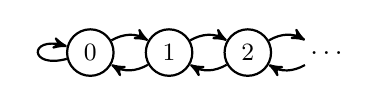
\begin{tikzpicture}[scale=1,>=stealth', auto, semithick,
      flat/.style={circle,draw=black,thick,text=black,font=\small}]
      \node[flat] (n0) at (0,0)  {$0$};
      \node[flat] (n1) at (1,0)  {$1$};
      \node[flat] (n2) at (2,0)  {$2$};
      \node[flat,white] (n3) at (3,0) {$ \ \ \ $};
      \node[] at (3,0) {$\ldots$};
      \draw[thick,->,bend left] (n0) to (n1);
      \draw[thick,->,bend left] (n1) to (n2);
      \draw[thick,->,bend left] (n2) to (n3);
      \draw[thick,->,loop left] (n0) to (n0);
      \draw[thick,->,bend left] (n1) to (n0);
      \draw[thick,->,bend left] (n2) to (n1);
      \draw[thick,->,bend left] (n3) to (n2);
    \end{tikzpicture}
  \end{center}
  where edges pointing right have probability $(1-\epsilon)/2$ and edges pointing left---including the loop at 0---have probability $(1+\epsilon)/2$. Examining the recursive description of $\rho(w)$, it is easy to confirm that the random variable $\rho(B_1, \ldots, B_n)$ is precisely given by the result of evolving the Markov chain above for $n$ steps with all probability initially placed at 0. It is further easy to confirm that the distribution given by~\eqref{eq:stationary} above is stationary for this chain.

  % The above Markov chain is \emph{irreducible} since every state is
  % reachable from every state.  In addition, it is easy to see that this
  % chain is \emph{aperiodic}---at time $n$, the walk visits every state
  % $s \in \{0, 1, \cdots, n\}$ with a strictly positive probability.
  % According to~\citep[Theorem 21.12]{LevinPeres}, an irreducible Markov
  % chain is positive recurrent if and only if there exists a distribution
  % $\pi$ on the state space satisfying $\pi P = \pi$, where $P$ is the
  % transition matrix of the chain.  We can take $\pi$ to be the
  % distribution given by~\eqref{eq:stationary}, implying that the chain
  % is positive recurrent.  Consequently, by ~\citep[Theorem
  % 21.14]{LevinPeres}, this irreducible, aperiodic, positive recurrent
  % Markov chain converges to the unique stationary distribution $\pi$.
  % It follows that the distributions $R_n$ limit to $R_\infty$.

  To establish stochastic dominance, it is convenient to work with the
  underlying distributions and consider walks of varying lengths: let
  $\DistRho_n: \Z \rightarrow \R$ denote the probability distribution given by
  $\rho(B_1, \ldots, B_n)$; likewise
  define $\DistRho_\infty$. For a distribution $\DistRho$ on $\Z$, we define $[\DistRho]_0$
  to denote the probability distribution obtained by shifting all
  probability mass on negative numbers to zero; that is, for $x \in \Z$,
  \[
    [\DistRho]_0(x) = \begin{cases} \DistRho(x) & \text{if $x > 0$},\\
      \sum_{t \leq 0} \DistRho(t) & \text{if $x = 0$},\\
      0 & \text{if $x < 0$.}
    \end{cases}
  \]
  We observe that if $A \dominatedby C$ then $[A]_0 \dominatedby [C]_0$ for any
  distributions $A$ and $C$ on $\Z$. It will also be convenient to
  introduce the shift operators: for a distribution
  $\DistRho: \Z \rightarrow \R$ and an integer $k$, we define $S^k\DistRho$ to be the
  distribution given by the rule $S^k\DistRho(x) = \DistRho(x-k)$. With these
  operators in place, we may write
  \[
    \DistRho_t = \left(\frac{1 - \epsilon}{2}\right) S^1 \DistRho_{t-1} +
      \left(\frac{1 + \epsilon}{2}\right) \left[S^{-1}\DistRho_{t-1} \right]_0\,,
  \]
  with the understanding that $\DistRho_0$ is the distribution placing unit probability at $0$. The proof now proceeds by induction. It is clear that $\DistRho_0 \dominatedby \DistRho_\infty$. Assuming that $\DistRho_n \dominatedby \DistRho_\infty$, we note that for any $k$
  \[
    S^k \DistRho_n \dominatedby S^k \DistRho_\infty \qquad \text{and, additionally, that
    }\qquad [S^{-1}\DistRho_n]_0 \dominatedby [S^{-1}\DistRho_{\infty}]_0\,.
  \]
  Finally, it is clear that stochastic dominance respects convex combinations, 
  in the sense that if $A_1 \dominatedby C_1$ and $A_2 \dominatedby C_2$ then 
  $\lambda A_1 + (1-\lambda) A_2 \dominatedby \lambda C_1 + (1-\lambda) C_2$ (for $0 \leq \lambda \leq 1$). We conclude that
  \[
    \DistRho_{t+1} = \left(\frac{1 - \epsilon}{2}\right) S^1 \DistRho_{t} +
      \left(\frac{1 + \epsilon}{2}\right) \left[S^{-1}\DistRho_{t} \right]_0 \dominatedby \left(\frac{1 - \epsilon}{2}\right) S^1 \DistRho_{\infty} +
      \left(\frac{1 + \epsilon}{2}\right) \left[S^{-1}\DistRho_{\infty} \right]_0 
      \,.
  \]
  By inspection, the right-hand side equals $\DistRho_{\infty}$, as desired. 
  Hence $\rho(B) \dominatedby R_\infty$.
  % $\qedhere$
\end{proof}

  \Paragraph{Remark.} 
  In fact, the random variable $\rho(B)$
  actually converges to $R_\infty$ as $n \rightarrow \infty$. 
  This can be seen, for example, 
  by solving for the stationary distribution of the Markov chain in the proof above. 
  However, we will only require the dominance for our exposition. 
  Importantly, since $\mu_x(\varepsilon) = \rho(x)$, and 
  $\Pr[\mu_x(y) \geq 0]$ increases monotonically 
  with an increase in $\Pr[\mu_x(\varepsilon) \geq r]$ for any $r \geq 0$, 
  it suffices to take $|x| \rightarrow \infty$ 
  when reasoning about an upper bound on $\Pr[\mu_x(y) \geq 0]$. 

%=======================================================
%=======================================================
\section{Proof of Bound~\ref{bound:analytic}}\label{sec:gf-proof}

%\begin{proof}[of Bound~\ref{bound:analytic}]
% \begin{proof}
  Anticipating the proof, we make a few remarks about generating
  functions and stochastic dominance.  We reserve the term
  \emph{generating function} to refer to an ``ordinary'' generating
  function which represents a sequence $a_0, a_1, \ldots$ of
  non-negative real numbers by the formal power series
  $\gf{A}(Z) = \sum_{t = 0}^\infty a_t Z^t$. When
  $\gf{A}(1) = \sum_t a_t = 1$ we say that the generating function is
  a \emph{probability generating function}; in this case, the
  generating function $\gf{A}$ can naturally be associated with the
  integer-valued random variable $A$ for which $\Pr[A = k] = a_k$. If
  the probability generating functions $\gf{A}$ and $\gf{B}$ are
  associated with the random variables $A$ and $B$, it is easy to
  check that $\gf{A} \cdot \gf{B}$ is the generating function
  associated with the convolution $A + B$ (where $A$ and $B$ are
  assumed to be independent).  Translating the notion of stochastic
  dominance to the setting with generating functions, we say that the
  generating function $\gf{A}$ \emph{stochastically dominates}
  $\gf{B}$ if $\sum_{t \leq T} a_t \leq \sum_{t \leq T} b_t$ for all
  $T \geq 0$; we write $\gf{B} \dominatedby \gf{A}$ to denote this state of
  affairs. If $\gf{B}_1 \dominatedby \gf{A}_1$ and
  $\gf{B}_2 \dominatedby \gf{A}_2$ then
  $\gf{B}_1 \cdot \gf{B}_2 \dominatedby \gf{A}_1 \cdot \gf{A}_2$ and
  $\alpha \gf{B}_1 + \beta \gf{B}_2 \dominatedby \alpha \gf{A}_1 + \beta
  \gf{A}_2$ (for any $\alpha, \beta \geq 0$).  Moreover, if
  $\gf{B} \dominatedby \gf{A}$ then it can be checked that
  $\gf{B}(\gf{C}) \dominatedby \gf{A}(\gf{C})$ for any probability
  generating function $\gf{C}(Z)$, where we write $\gf{A}(\gf{C})$ to
  denote the composition $\gf{A}(\gf{C}(Z))$.


  Finally, we remark that
  if $\gf{A}(Z)$ is a generating function which converges as a
  function of a complex $Z$ for $|Z| < R$ for some non-negative $R$, 
  $R$ is called the \emph{radius of convergence} of $\gf{A}$.  
  It follows from \citep[Theorem 2.19]{WilfGF} that 
  $\lim_{k \rightarrow \infty} {a_k}R^k = 0$ and $|a_k| = O(R^{-k})$. 
	In addition, if $\gf{A}$ is a probability generating function associated with the
  random variable $A$ then it follows that
  $\Pr[A \geq T] = O(R^{-T})$.
  
  We define $p = (1 - \epsilon)/2$ and $q = 1 - p$ and 
  as in the proof of Bound~\ref{bound:geometric},
  consider the independent $\{0,1\}$-valued random variables
  $w_1, w_2, \ldots$ where $\Pr[w_t = 1] = p$. We also define the
  associated $\{\pm1\}$-valued random variables $W_t =
  (-1)^{1+w_t}$.
	
  
	Although our actual interest is in the random variable $\mu_x(y)$ 
	from~\eqref{eq:mu-relative-recursive} on a characteristic string $w=xy$, 
  we begin by analyzing the case when $|x|=0$. 

  %\vspace{-2ex}
	\Paragraph{Case 1: $x$ is the empty string.}
  In this case, the random variable $\mu_x(y)$ is identical to $\mu(w)$ 
  from~\eqref{eq:mu-recursive} with $w = y$. 
	Our strategy is to study the probability generating
  function
  \[
    \gf{L}(Z) = \sum_{t = 0}^\infty \ell_t Z^t
  \]
  where $\ell_t = \Pr[\text{$t$ is the last time $\mu_t =
    0$}]$. Controlling the decay of the coefficients $\ell_t$ suffices
  to give a bound on the probability that $w_1\ldots w_k$ is forkable
  because
  \[
    \Pr[\text{$w_1 \ldots w_k$ is forkable}] \leq 1 - \sum_{t =
      0}^{k-1} \ell_t = \sum_{t = k}^\infty \ell_t\,.
  \]
  It seems challenging to give a closed-form algebraic expression for
  the generating function $\gf{L}$; our approach is to develop a
  closed-form expression for a probability generating function
  $\gf{\hat{L}} = \sum_t \hat{\ell}_t Z^t$ which stochastically
  dominates $\gf{L}$ and apply the analytic properties of this closed
  form to bound the partial sums $\sum_{t \geq k} \hat{\ell}_k$.
  Observe that if $\gf{L} \dominatedby \gf{\hat{L}}$ then the series
  $\gf{\hat{L}}$ gives rise to an upper bound on the probability that
  $w_1\ldots w_k$ is forkable as
  $\sum_{t=k}^\infty \ell_t \leq \sum_{t=k}^\infty \hat{\ell}_t$.

  The coupled random variables $\rho_t$ and $\mu_t$ are Markovian
  in the sense that values $(\rho_s, \mu_s)$ for $s \geq t$ are
  entirely determined by $(\rho_t, \mu_t)$ and the subsequent
  values $W_{t+1}, \ldots$ of the underlying variables $W_i$. We
  organize the sequence
  $(\rho_0, \mu_0), (\rho_1, \mu_1), \ldots$ into ``epochs''
  punctuated by those times $t$ for which $\rho_t = \mu_t =
  0$. With this in mind, we define $\gf{M}(Z) = \sum m_t Z^t$ to be
  the generating function for the first completion of such an epoch,
  corresponding to the least $t > 0$ for which
  $\rho_t = \mu_t = 0$. As we discuss below, $\gf{M}(Z)$ is not a
  probability generating function, but rather
  $\gf{M}(1) = 1 - \epsilon$. It follows that
  \begin{equation}\label{eq:L-def}
    \gf{L}(Z) = \epsilon(1 + \gf{M}(Z) + \gf{M}(Z)^2 + \cdots) =
    \frac{\epsilon}{1 - \gf{M}(Z)}\,.
  \end{equation}
  Below we develop an analytic expression for a generating function
  $\gf{\hat{M}}$ for which $\gf{M} \dominatedby \gf{\hat{M}}$ and define
  $\gf{\hat{L}} = \epsilon/(1 - \gf{\hat{M}}(Z))$. We then proceed as
  outlined above, noting that $\gf{L} \dominatedby \gf{\hat{L}}$ and using
  the asymptotics of $\gf{\hat{L}}$ to upper bound the probability
  that a string is forkable.

  In preparation for defining $\gf{\hat{M}}$, we set down two
  elementary generating functions for the ``descent'' and ``ascent''
  stopping times. Treating the random variables $W_1, \ldots$ as
  defining a (negatively) biased random walk, define $\gf{D}$ to be
  the generating function for the \emph{descent stopping time} of the
  walk; this is the first time the random walk, starting at 0, visits
  $-1$. The natural recursive formulation of the descent time yields a
  simple algebraic equation for the descent generating function,
  $\gf{D}(Z) = qZ + pZ \gf{D}(Z)^2$, and from this we may conclude
  \[
    \gf{D}(Z) = \frac{1 - \sqrt{1 - 4pqZ^2}}{2pZ}\,.
  \]
  We likewise consider the generating function $\gf{A}(Z)$ for the
  \emph{ascent stopping time}, associated with the first time the
  walk, starting at 0, visits 1: we have
  $\gf{A}(Z) = pZ + qZ \gf{A}(Z)^2$ and
  \[
    \gf{A}(Z) = \frac{1 - \sqrt{1 - 4pqZ^2}}{2qZ}\,.
  \]
  Note that while $\gf{D}$ is a probability generating function, the
  generating function $\gf{A}$ is not: according to the classical
  ``gambler's ruin'' analysis~\cite{Grinstead:1997ng}, the probability
  that a negatively-biased random walk starting at 0 ever rises to 1
  is exactly $p/q$; thus $\gf{A}(1) = p/q$.

  Returning to the generating function $\gf{M}$ above, we note that an
  epoch can have one of two ``shapes'': in the first case, the epoch
  is given by a walk for which $W_1 = 1$ followed by a descent (so
  that $\rho$ returns to zero); in the second case, the epoch is
  given by a walk for which $W_1 = -1$, followed by an ascent (so that
  $\mu$ returns to zero), followed by the eventual return of $\rho$
  to 0. Considering that when $\rho_t > 0$ it will return to zero
  in the future almost surely, it follows that the probability that
  such a biased random walk will complete an epoch is
  $p + q(p/q) = 2p = 1 - \epsilon$, as mentioned in the discussion
  of~\eqref{eq:L-def} above. One technical difficulty arising in a
  complete analysis of $\gf{M}$ concerns the second case discussed
  above: while the distribution of the smallest $t > 0$ for which
  $\mu_t = 0$ is proportional to $\gf{A}$ above, the distribution of
  the smallest subsequent time $t'$ for which $\rho_{t'} = 0$
  depends on the value $t$. More specifically, the distribution of the
  return time depends on the value of $\rho_t$. Considering that
  $\rho_t \leq t$, however, this conditional distribution (of the
  return time of $\rho$ to zero conditioned on $t$) is
  stochastically dominated by $\gf{D}^t$, the time to descend $t$
  steps. This yields the following generating function $\gf{\hat{M}}$
  which, as described, stochastically dominates $\gf{M}$:
  \[
    \gf{\hat{M}}(Z) = pZ\cdot \gf{D}(Z) + qZ \cdot \gf{D}(Z) \cdot
    \gf{A}(Z\cdot \gf{D}(Z))\,.
  \]
  
  It remains to establish a bound on the radius of convergence of
  $\gf{\hat{L}}$. Recall that if the radius of convergence of
  $\gf{\hat{L}}$ is $\exp(\delta)$ it follows that
  $\Pr[\text{$w_1 \ldots w_k$ is forkable}] = O(\exp(-\delta k))$. A
  sufficient condition for convergence of
  $\gf{\hat{L}}(z) = \epsilon/(1 - \gf{\hat{M}}(z))$ at $z$ is that
  that all generating functions appearing in the definition of
  $\gf{\hat{M}}$ converge at $z$ and that the resulting value
  $\gf{\hat{M}}(z) < 1$.
  
  The generating function $\gf{D}(z)$ (and $\gf{A}(z)$) converges when
  the discriminant $1 - 4pqz^2$ is positive; equivalently
  $|z| < 1/\sqrt{1 - \epsilon^2}$ or
  $|z| < 1 + \epsilon^2/2 + O(\epsilon^4)$. Considering
  $\gf{\hat{M}}$, it remains to determine when the second term,
  $qz D(z) \gf{A}(z \gf{D}(z))$, converges; this is likewise determined by
  positivity of the discriminant, which is to say that
  \[
    1 - (1 - \epsilon^2)\left(\frac{1 - \sqrt{1 - (1 - \epsilon^2)z^2}}{1 - \epsilon}\right)^2 > 0\,.
  \]
  Equivalently,
  \[
    |z| <  \sqrt{\frac{1}{1 + \epsilon}\left(\frac{2}{\sqrt{1 - \epsilon^2}} - \frac{1}{1+\epsilon}\right)} = 1 + \epsilon^3/2 + O(\epsilon^4) 
		\, .	
  \]
  Note that when the series $pz \cdot \gf{D}(z)$ converges, it
  converges to a value less than $1/2$; the same is true of
  $qz \cdot \gf{A}(z)$. It follows that for
  $|z| = 1 + \epsilon^3/2 + O(\epsilon^4)$, $|\gf{\hat{M}}(z)| < 1$
  and $\gf{\hat{L}}(z)$ converges, as desired. We conclude that
	\begin{align}
	  \Pr[\text{$w_1 \ldots w_k$ is forkable}] &= \exp(-\epsilon^3(1 + O(\epsilon))k/2)\,.
	\label{eq:prob_forkable_gf}
	\end{align}

          %\vspace{-2ex}
	\Paragraph{Case 2: $x$ is non-empty.}
        The relative margin before $y$ begins is $\mu_x(\varepsilon)$.
        Recalling that $\mu_x(\varepsilon) = \rho(x)$ and conditioning on the event that $\rho(x) = r$, 
    let us define the random variables $\left\{ \tilde{\mu}_t \right\}$ for $t = 0, 1, 2, \cdots$ as follows: $\tilde{\mu}_0 = \rho(x)$ and
    \[
      %\, , \qquad \text{and} \qquad
      \Pr[\tilde{\mu}_t = s]\, =\, \Pr[\mu_x(y) = s \mid \rho(x) = r \text{ and } |y| = t ]
      \, .
    \]
    If the $\tilde{\mu}$ random walk makes the $r$th descent at some time $t < n$, then $\tilde{\mu}_t = 0$ and the remainder of the walk is 
	identical to an $(k-t)$-step $\mu$ random walk which we have already analyzed. 
	Hence we investigate the probability generating function
	\[
			\gf{B}_r(Z) = \gf{D}(Z)^r \gf{L}(Z) \quad \text{with coefficients} \quad
      b^{(r)}_t := \Pr[t \text{ is the last time } \tilde{\mu}_t = 0 \mid \tilde{\mu}_0 = r]	
  \]
  where $t = 0, 1, 2, \cdots$. Our interest lies in the quantity 
    \[
      b_t 
      := \Pr[t \text{ is the last time } \tilde{\mu}_t = 0] 
      = \sum_{r\geq 0}{  b^{(r)}_t \DistRho_m(r) } 
      \,,
     \]
  where the \emph{reach distribution} 
  $\DistRho_m : \Z \rightarrow [0,1]$ 
  associated with the random variable $\rho(x), |x| = m$ is defined as 
  \begin{align}\label{eq:dist-rho}
    % \DistRho_m(r) &= \Pr_{W \sim \mathcal{D}}[\rho(W) = r \Given W \text{ has length } m]
    \DistRho_m(r) &= \Pr_{x \SuchThat |x| = m}[\rho(x) = r]
    \, .
  \end{align}
     % from~\eqref{eq:dist-rho}.
     Let $\gf{R}_m(Z)$ be the probability generating function
     for the distribution $\DistRho_m$. 
     Using Lemma~\ref{lemma:rho-stationary} and Definition~\ref{def:dominance}, we deduce that
     $\gf{R}_m \dominatedby \gf{R}_\infty$ for every $m \geq 0$ since 
    $\DistRho_m \dominatedby \StationaryRho$.
     In addition, it is easy to check from~\eqref{eq:stationary} that
     the probability generating function for $\StationaryRho$ is in fact
     $\gf{R}_\infty(Z) = (1-\beta)/(1-\beta Z)$ where $\beta := (1-\epsilon)/(1+\epsilon)$. 
    Thus the generating function corresponding to the
     probabilities $\{b_t\}_{t=0}^\infty$ is
	\begin{align}
		\gf{B}(Z) 
		&= \sum_{t=0}^\infty{b_t Z^t} = \sum_{r=0}^\infty{\DistRho_m(r) \sum_{t=0}^\infty{b_t^{(r)} Z^t} } = \sum_{r=0}^\infty{\DistRho_m(r) \gf{B}_r(Z) } \nonumber \\
    &= \gf{L}(Z) \sum_{r=0}^\infty{\DistRho_m(r) \gf{D}(Z)^r}    \nonumber 
		= \gf{L}(Z)\  \gf{R}_m (\gf{D}(Z)) \nonumber 
		\dominatedby \gf{\hat{L}}(Z)\  \gf{R}_\infty (\gf{D}(Z))  \nonumber \\
    &= \frac{(1-\beta)\,\gf{\hat{L}}(Z) }{1 - \beta \gf{D}(Z)}
		\, .
	\label{eq:gf-mu-relative}
	\end{align}
  The dominance notation above follows because
  $\gf{L} \dominatedby \gf{\hat{L}}$ and $\gf{R}_m \dominatedby \gf{R}_\infty$.


  For $\gf{B}(Z)$ to converge, we need to check that $\gf{D}(Z)$
  should never converge to $1/\beta$.  One can easily check that
  the radius of convergence of $\gf{D}(Z)$---which is
  $\displaystyle 1/\sqrt{1-\epsilon^2}$---is strictly less than $1/\beta$ when
  $\epsilon > 0$.  We conclude that $\gf{B}(Z)$ converges if
  both $\gf{D}(Z)$ and $\gf{L}(Z)$ converge.  The radius of
  convergence of $\gf{B}(Z)$ would be the smaller of the radii
  of convergence of $\gf{D}(Z)$ and $\gf{L}(Z)$.  We already
  know from the previous analysis that $\gf{\hat{L}}(Z)$ has the
  smaller radius of the two; therefore, the bound
  in~\eqref{eq:prob_forkable_gf} applies to the relative margin $\mu_x(y)$
  for $|x|\geq 0$. 
  \hfill $\qed$  
  % $\qedhere$
  % $\qed$
% \end{proof}


%=======================================================
\section{Proof of Bound~\ref{bound:geometric}}\label{sec:martingale-proof-new}

Let $\epsilon \in (0, 1)$,  
$W \in \{0,1\}^m, W^\prime \in \{0,1\}^k$ 
where both $(W_1, \ldots, W_n)$ and $(W^\prime_1, \ldots, W^\prime_n)$ 
satisfy the $\epsilon$-martingale condition. 
Let $B \in \{0,1\}^m, B^\prime \in \{0,1\}^k$ where the components of $B, B^\prime$ 
are independent with expectation $(1 - \epsilon)/2$.
By Lemma~\ref{lemma:rho-stationary}, 

\begin{equation*}\label{eq:WB-dominance}\tag{$*$}
  W \dominatedby B\quad \text{and} \quad W^\prime \dominatedby B^\prime
  \,. 
\end{equation*}

Let us define the partial order $\leq$ on Boolean strings $\{0,1\}^k, k \in \NN$ 
as follows: 
$a \leq b$ if and only if
for all $i \in [k]$, $a_i = 1$ implies $b_i = 1$. 
Let $\mu : \{0,1\}^k \rightarrow \Z$ be the margin function 
from Lemma~\ref{lem:relative-margin}. 
Observe that for Boolean strings $a, a^\prime, b, b^\prime$ 
with $|a| = |a^\prime|$ and $|b| = |b^\prime|$, 
(i.) $b \leq b^\prime$ implies $\mu_a(b) \leq \mu_a(b^\prime)$ and 
(ii.) $a \leq a^\prime$ implies $\mu_a(b) \leq \mu_{a^\prime}(b)$. 
That is, 
\begin{equation*}\label{eq:mu-WB-dominance}\tag{$\dagger$}
  \text{$\mu_a(b)$ is non-decreasing in both $a$ and $b$}
  \,.   
\end{equation*}

Using~\eqref{eq:WB-dominance} and~\eqref{eq:mu-WB-dominance}, 
it follows that $\mu_W(W^\prime) \dominatedby \mu_{B}(B^\prime)$. 
% Recall that $P \dominatedby Q$ is true if, 
% for all monotone sets $E$, 
% by $\Pr[ P \in E ] \leq \Pr[Q \in E]$. 
% In particular, concerning the dominance $\mu_W(W^\prime) \dominatedby \mu_{B}(B^\prime)$, 
Writing $x = W$ and $y = W^\prime$, we have 
\begin{align*}
  \Pr[\mu_x(y) \geq 0]\, 
    = \Pr[\mu_W(W^\prime) \geq 0]\, 
    \leq \Pr[\mu_{B}(B^\prime) \geq 0]
\end{align*}
where the inequality comes from the definition of stochastic dominance. 
A bound on the right-hand side 
is obtained in Bound~\ref{bound:analytic}. 
\hfill $\qed$






In \Section~\ref{sec:martingale-proof}, 
we present a weaker bound 
on $\Pr[\mu_x(y) \geq 0]$ where the sequence 
$x_1, \ldots, x_m, y_1, \ldots, y_k$ satisfies $\epsilon$-martingale conditions. 
The proof directly uses the properties of the martingale 
and Azuma's inequality  but 
it does not use a stochastic dominance argument. 
Although it gives a bound of $3 \exp\left( -\epsilon^4 (1 - O(\epsilon) ) k/64 \right)$, 
the reader might find the proof of independent interest. 


%
% The following lemma shows that $W$ is, in fact, 
% dominated by $B = (B_1, \ldots, B_k)$ where 
% each $B_i$ is an independent Bernoulli random variable 
% with parameter $(1 - \epsilon)/2$.
%
%--------------------------------
% \begin{lemma}\label{lem:dominance}
%   Let $X = (X_1, \ldots, X_n)$ be a family of random variables taking
%   values in $\{0,1\}$ with the property that, for each $i > 0$,
%   $\Exp[X_i \mid X_1, \ldots, X_{i-1}] \leq p$. Let
%   $B = (B_1, \ldots, B_n)$ be a family of independent random
%   variables, taking values in $\{0,1\}$, for which
%   $\Exp[B_i = 1] = p$.  Then $X \dominatedby B$.
% \end{lemma}
%
% \begin{proof}
%   We proceed by induction. The statement is clear for $n=1$. In
%   general, consider a random variable $X$ satisfying the conditions of
%   the theorem and taking values in $\{0,1\}^{n+1}$; let
%   $E \subset \{0,1\}^{n+1}$ be a monotone event. We wish to prove that
%   $\Pr[X \in E] \leq \Pr[B \in E]$.
%
%   We write $X = (Y, Z)$, where $Y$ takes values in $\{0,1\}^n$ and $Z$
%   in $\{0,1\}$. By induction, we may assume that
%   $Y \dominatedby (B_1, \ldots, B_n)$. Consider the events
%   \[
%     E_0 = \{ (y_1, \ldots, y_n) \mid (y_1, \ldots, y_n, 0) \in
%     E\}\qquad\text{and}\qquad E_1 = \{ (y_1, \ldots, y_n) \mid (y_1,
%     \ldots, y_n, 1) \in E\}\,;
%   \]
%   observe that the monotonicity of $E$ implies that
%   $E_0 \subseteq E_1$ and that $E_0, E_1$ are monotone. 
%   To study
%   $\Pr[X \in E]$, for an element
%   $y = (y_1, \ldots, y_n) \in \{0,1\}^n$ define
%   \[
%     q(y) = \Pr[ X \in E \mid Y = y]\,.
%   \]
%   Observe that $\Pr[X \in E] = \Exp[q(Y)]$ and, recalling that
%   $E_0 \subset E_1$, that
%   \begin{align*}
%     y \in E_0 & \Rightarrow q(y) = 1,\\
%     y \in E_1 \setminus E_0 & \Rightarrow q(y) \leq p\quad\text{by assumption, and}\\
%     y \not\in E_1 & \Rightarrow q(y) = 0\,.
%   \end{align*}
%   We conclude that
%   \begin{align}
%     \Pr[X \in E] & \leq \Pr[Y \in E_0] + p\cdot
%                    \Pr[Y \in E_1 \setminus E_0]
%                    = p \Pr[Y \in E_1] + (1-p) \Pr[Y \in E_0] \nonumber\\
%                  & \leq p \Pr[(B_1, \ldots, B_n) \in E_1] + (1-p) \Pr[(B_1, \ldots, B_n) \in E_0] \label{eq:XBdominance}\\
%                  &= \Pr[(B_1, \ldots, B_n) \in E_0] + p \Pr[(B_1, \ldots, B_n) \in E_1 \setminus E_0] = \Pr[B \in E]\,, \nonumber
%   \end{align}
%   as desired. The inequality of line~\eqref{eq:XBdominance} follows by
%   the induction hypothesis.
% \end{proof}
% ---------------------------------




\section{Proof of main theorems}\label{sec:thm-proofs}

\Paragraph{Proof of Theorem~\ref{thm:main}.}

Let us start with the following observation.
It allows us to formulate the
$(s, k)$-settlement insecurity of a distribution $\Distribution$
directly in terms of the relative margin.

\begin{lemma}\label{lemma:settlement-margin}
  Let $s, k, T \in \NN$. 
  Let $\Distribution$ be any distribution on $\{0,1\}^T$. 
  Then
  \[
    \mathbf{S}^{s,k}[\Distribution] \leq
      \Pr_{w \sim \Distribution} \left[\parbox{65mm}{
          there is a decomposition $w = x y z$, 
          where $|x| = s - 1$ and $|y| \geq k + 1$, 
          so that $\mu_x(y) \geq 0$
      }\right]
    \,.
  \]
\end{lemma}
\begin{proof}
  Lemma~\ref{lem:main-forks} implies that 
  $\mathbf{S}^{s,k}[\Distribution]$ is no more than 
  the probability that slot $s$ is not $k$-settled 
  for the characteristic string $w$. 
  By Observation~\ref{obs:settlement-balanced-fork}, 
  this probability, in turn, is no more than 
  the probability that there exists an $x$-balanced fork 
  $F \Fork xy$
  where we write $w = xyz, |x| = s - 1, |y| \geq k + 1, |z| \geq 0$. 
  Finally, Fact~\ref{fact:margin-balance} states that 
  for any characteristic string $xy$, 
  the two events ``exists an $x$-balanced fork $F \Fork xy$'' 
  and ``$\mu_x(y)$ is non-negative'' have the same measure. 
  Hence the claim follows. 
\end{proof}

If the distribution $\mathcal{D}$ in the lemma above 
satisfies the $\epsilon$-martingale condition, 
the probability in this lemma is no more than the probability 
in the left-hand side of Corollary~\ref{cor:main}. 
Finally, by retracing the proof of Corollary~\ref{cor:main} 
using the explicit probability from Bound~\ref{bound:geometric}, 
we see that the bound in Corollary~\ref{cor:main} is 
$O(1) \cdot \exp\bigl(-\Omega(\epsilon^3 (1 - O(\epsilon))k)\bigr)$. 
Since $\mathcal{B}_\epsilon$ satisfies the $\epsilon$-martingale condition, 
we conclude that $\mathbf{S}^{s,k}[\mathcal{B}_\epsilon]$ is no more than 
this quantity as well.
% \[
%   \mathbf{S}^{s,k}[\mathcal{B}_\epsilon] 
%       \leq O(1) \cdot \exp\bigl(-\Omega(\epsilon^3 (1 - O(\epsilon))k)\bigr)
%     \,.
% \]


For any player playing the settlement game, 
the set of strings on which the player wins is monotone 
with respect to the partial order $\leq$ defined in Section~\ref{sec:martingale-proof-new}. 
To see why, note that if the adversary wins with a specific string $w$, 
he can certainly win with any string $w^\prime$ where $w \leq w^\prime$. 
As $\mathcal{B}_\epsilon$ stochastically dominates $\mathcal{W}$, it follows that 
$
  \mathbf{S}^{s,k}[\mathcal{W}] \leq \mathbf{S}^{s,k}[\mathcal{B}_\epsilon]
$.

\hfill$\qed$


\Paragraph{Proof of Theorem~\ref{thm:main-CP}}
For the first inequality, observe that if $w$ violates $\kCP$, it must violate $\kSlotCP$ as well. 
It remains to prove the second inequality. 
Let $\Distribution$ be any distribution on $\{0,1\}^T$. 
We can apply Fact~\ref{fact:margin-balance} on the statement of Theorem~\ref{thm:cp-fork} 
to deduce that 
\begin{equation*}\label{eq:main-argument-1}
  \Pr_{w \sim \Distribution}[\text{$w$ violates $\kSlotCP$}] 
    \leq 
% \Pr_{\substack{w = x y z \\ |y| \geq k + 1} }[\text{exists a $k$-settlement violation} ] 
%    = 
    \Pr_{w \sim \Distribution}\left[\parbox{55mm}{
      there is a decomposition $w = xyz$, 
      where $|y| \geq k$, 
      so that $\mu_x(y) \geq 0$ 
    } \right] 
    \,.
\end{equation*}
By using a union bound over $|x|$, the above probability is at most 
\[
    \sum_{s = 1}^{T - k + 1} 
    \quad 
      \Pr_w\left[\parbox{60mm}{
        there is a decomposition $w = xyz$, 
        where $|x| = s - 1$ and $|y| \geq k$, 
        so that $\mu_x(y) \geq 0$ 
      }\right] 
    \,.
\]
Since $w$ satisfies the $\epsilon$-martingale condition, 
we can upper bound the probability inside the sum 
using Corollary~\ref{cor:main}. 
As we have seen in the proof of Theorem~\ref{thm:main}, 
the bound in Corollary~\ref{cor:main} is 
$
  O(1) \cdot \exp\bigl(-\Omega(\epsilon^3 (1 - O(\epsilon))k)\bigr)
  % \,.
$.
It follows that the sum above is at most $T \exp\bigl(-\Omega(\epsilon^3 (1 - O(\epsilon))k)\bigr)$.
\hfill $\qed$


It remains to prove the recursive formulation of the relative margin 
from \Section~\ref{sec:recursion}; 
we tackle it in the next section.



%%% Local Variables:
%%% mode: latex
%%% TeX-master: "main"
%%% End:


\section{An optimal online adversary against slot settlement}
\label{sec:recursion}
In this section, we introduce additional elements of the fork framework from~\citet{LinearConsistency}, 
most notably the notions of ``reach'' and ``relative margin.'' 
We show that relative margin is just as expressive 
as the Catalan slots 
for characterizing slot settlement. 
Next, we prove a recurrence relation for relative margin; 
it can be used to compute 
the probability that a given slot is $k$-settled, 
when the symbols of the characteristic string are i.i.d\ .
Finally, we present an adversary who, 
given a characteristic string one symbol at a time, 
optimally attacks the settlement of all slots at once. 



\subsection{Closed forks, reach, and extensions}
\begin{definition}[Closed fork]
  A fork $F$ is \emph{closed} if every leaf is honest. For convenience, we say the trivial fork is closed.
\end{definition}
Closed forks have two nice properties that make them especially useful in reasoning about the view of honest parties.
First, 
all honest observers will select a unique longest tine from this fork 
(since all longest tines in a closed fork are honest, 
honest parties are aware of all previous honest blocks, 
they observe the longest chain rule, and they employ the same consistent tie-breaking rule).  
Second, 
% recalling our description of the
% settlement game, 
closed forks intuitively capture decision points for the adversary.
The adversary can potentially show many tines to many honest parties, 
but once an honest node has been placed on top of 
a tine, any adversarial blocks beneath it are part of the public record and are visible to all honest parties. 
For these
reasons, we will often find it easier to reason about closed forks than arbitrary forks. % (without loss of generality).

The next few definitions are the start of a general toolkit for reasoning about an adversary's capacity to build highly diverging paths in forks, based on the underlying characteristic string.
%current state of a fork.

%%%%Reach and margin
\begin{definition}[Gap, reserve, and reach]\label{def:gap-reserve-reach-mh}
For a closed fork $F \vdash w$ and its unique longest tine $\hat{t}$, we define the \emph{gap} of a tine $t$ to be $\gap(t)=\length(\hat{t})-\length(t)$.
Furthermore, we define the \emph{reserve} of $t$, denoted $\reserve(t)$, to be the number of adversarial indices in $w$ that appear after the terminating vertex of $t$. More precisely, if $v$ is the last vertex of $t$, then
\[
  \reserve(t)=|\{\ i \mid w_i=1 \ and \ i > \ell(v)\}|\,.
  \]
These quantities together define the \emph{reach} of a tine: $
\reach(t)=\reserve(t)-\gap(t)$.
\end{definition}

The notion of reach can be intuitively understood as a measure of
the resources available to our adversary in the settlement
game. Reserve tracks the number of slots in which the adversary has
the right to issue new blocks.  When reserve exceeds gap (or
equivalently, when reach is nonnegative), such a tine could be
extended---using a sequence of dishonest blocks---until it is as long
as the longest tine. Such a tine could be offered to an honest player
who would prefer it over, e.g., the current longest tine in the
fork. In contrast, a tine with negative reach is too far behind to be
directly useful to the adversary at that time.

\begin{definition}[Maximum reach]
For a closed fork $F\vdash w$, we define $\rho(F)$ to be the largest reach attained by any tine of $F$, i.e., 
\[
\rho(F)=\underset{t}\max \ \reach(t)\,.
\]
Note that $\rho(F)$ is never negative (as the longest tine of any fork always has reach at least 0). We overload this notation to denote the maximum reach over all forks for a given characteristic string: 
\[
\rho(w)=\underset{\substack{F\vdash w\\\text{$F$ closed}}}\max\big[\underset{t}\max \ \reach(t)\big]\,.
\]
\end{definition}

Reach of vertices is always non-increasing as we move down a tine. 
That is, if $B_1, B_2, \ldots$ are vertices on the same tine in the root-to-leaf order, then 
$\reach(B_i) \leq \reach(B_{i+1})$. 
The inequality is strict if $B_{i + 1}$ is honest. 
Consequently, the reach of an adversarial tine is no more than 
the reach of the last honest vertex in that tine. 
In any fork, the reach of a maximum-length tine is always non-negative. 
Hence, an honest tine with the maximum length over all honest tines 
will always have a non-negative reach. 
Thanks to the monotonicity of the honest-depth function $\hdepth(\cdot)$, 
if there are multiple honest tines 
having the (same) maximum length among all honest tines, 
they must have the same label. 
Therefore, if $h$ is the last honest slot in $w$ and 
$t$ a maximum-length honest tine with label $h$,  
then $\reach(t) \geq 0$. 


% {\color{red} Fix this.}
% \begin{fact}\label{fact:fork-structure-reach}
%   Let $w \in \{\h, \H, \A\}^T$ be a characteristic string, 
%   $s \in [T + 1]$ be an integer, 
%   $x \PrefixEq w, |x| = s - 1$. 
%   Let 
%   $F$ be a fork for $w$, 
%   $B$ an honest vertex in $F$, 
%   $h = \ell(B)$, and 
%   $I = [h + 1, s - 1]$.
%   Let $F_x \Fork x$ be a fork prefix of $F$ so that 
%   $F_x$ contains all honest tines from $F$ with labels at most $s - 1$. 
%   The following statements are equivalent: 
%   \begin{enumerate*}[label=(\roman*)]
%     \item \label{fact-reach-part:Aheavy} $I$ is $\Aheavy$; 
%     \item \label{fact-reach-part:viable-adv-ext} 
%       $B$ has an adversarial extension $t, \ell(t) \in I$ so that $t$ is 
%       viable at the onset of slot $s$; and
%     \item \label{fact-reach-part:nonneg-reach} $\reach_{F_x}(B) \geq 0$;
%   \end{enumerate*}      
% \end{fact}
% \begin{proof}
%   The equivalence between items~\ref{fact-reach-part:Aheavy} and~\ref{fact-reach-part:viable-adv-ext} has already been shown in Fact~\ref{fact:fork-structure}. 
%   \begin{description}[font=\normalfont\itshape\space]

%     \item[\ref{fact-reach-part:nonneg-reach} implies~\ref{fact-reach-part:Aheavy}.]
%       By assumption, $\reach_{F_x}(B)  = \reserve_{F_x}(B) - \gap_{F_x}(B) \geq 0$.               
%       Since $\reserve_{F_x}(B) = \#_\A(I)$ and $\gap_{F_x}(B) \geq \#_\h(I) + \#_\H(I)$, 
%       it follows that $\#_\A(I) \geq \#_\h(I) + \#_\H(I)$. 

%     \item[\ref{fact-reach-part:viable-adv-ext} implies~\ref{fact-reach-part:nonneg-reach}.]
%       Since $t$ is an adversarial extension of $B$, 
%       it contains only adversarial vertices from $I$. 
%       By assumption, $t$ is viable at the onset of slot $s$.
%       It follows that $\#_\A(I) \geq \gap_{F_x}(B)$.
%       Since $\reserve_{F_x}(B) = \#_\A(I)$, we have 
%       $\reach_{F_x}(B) = \reserve_{F_x}(B) - \gap_{F_x}(B) \geq 0$.  
      
%   \end{description}            
% \end{proof}






\paragraph{Non-negative reach, $\A$-heaviness, and viable adversarial extensions.}
Let $w \in \{\h, \H, \A\}^T$,   
$s \in [T + 1]$, and 
$F \Fork w_1 \ldots w_{s - 1}$ an arbitrary fork. 
Let $B \in F$ be an honest vertex 
and $t$ a maximum-length tine in $F$.
Consider the following statements: 
\begin{enumerate}[label=(\alph*)]
  \item \label{fact-reach-part:viable-adv-ext} $B$ has an adversarial extension viable at the onset of slot $s$.
  \item \label{fact-reach-part:nonneg-reach} $\reach_{F}(B)$ is non-negative.
  \item \label{fact-reach-part:Aheavy} The interval $I = [\ell(B) + 1, s - 1]$ is $\Aheavy$. 
  \item \label{fact-reach-part:conservative} $\length(t) = \#_\h(I) + \#_\H(I) + \length(B)$.     
\end{enumerate}

\begin{fact}\label{fact:fork-structure-reach}
    ~\ref{fact-reach-part:viable-adv-ext} $\Longrightarrow$
    \ref{fact-reach-part:nonneg-reach} $\Longrightarrow$
    \ref{fact-reach-part:Aheavy}.
    In addition, if we assume~\ref{fact-reach-part:conservative}, then 
    ~\ref{fact-reach-part:Aheavy} $\Longrightarrow$ 
    ~\ref{fact-reach-part:nonneg-reach} $\Longrightarrow$
    ~\ref{fact-reach-part:viable-adv-ext}.
\end{fact}
Fact~\ref{fact:fork-structure-reach} can be seen as 
a refinement of Fact~\ref{fact:fork-structure} 
when $F$ is a closed fork. 
\begin{proof}~
  \begin{description}[font=\normalfont\itshape\space]
    \item[\ref{fact-reach-part:viable-adv-ext} implies~\ref{fact-reach-part:nonneg-reach}.]
      An adversarial extension of $B$ 
      contains only adversarial vertices from $I$. 
      If this extension is viable at the onset of slot $s$, 
      $\#_\A(I)$ must be at least $\gap_{F}(B)$.
      Since $\reserve_{F}(B) = \#_\A(I)$, we have 
      $\reach_{F}(B) = \reserve_{F}(B) - \gap_{F}(B) \geq 0$.  
      
    \item[\ref{fact-reach-part:nonneg-reach} implies~\ref{fact-reach-part:Aheavy}.]
      By assumption, $\reach_{F}(B)  = \reserve_{F}(B) - \gap_{F}(B) \geq 0$.               
      $t$ contains at least $\#_\h(I) + \#_\H(I)$ vertices from 
      the interval $I$; 
      hence, $\gap_{F}(B) \geq \#_\h(I) + \#_\H(I)$. 
      Since $\reserve_{F}(B) = \#_\A(I)$, 
      it follows that $\#_\A(I) \geq \#_\h(I) + \#_\H(I)$. 

    \item[\ref{fact-reach-part:conservative} and~\ref{fact-reach-part:Aheavy} implies~\ref{fact-reach-part:nonneg-reach}.]
      Since $I$ is $\Aheavy$, 
      $\reserve_F(B) = \#_\A(I) \geq \#_\h(I) + \#_\H(I)$. 
      However, since~\ref{fact-reach-part:conservative} holds, 
      the latter quantity equals $\length(t) - \length(B) = \gap_F(B)$. 
      It follows that $\reach_F(B) = \reserve_F(B) - \gap_F(B) \geq 0$. 

    \item[\ref{fact-reach-part:conservative} and~\ref{fact-reach-part:nonneg-reach} implies~\ref{fact-reach-part:viable-adv-ext}.]
      $I$ contains at least $\gap_F(B)$ adversarial slots. 
      We can use these slots augment $B$ 
      into an adversarial tine $t'$ 
      of length at least $\length(t)$. 
      Thus $t'$ will be viable at the onset of slot $s$.
  \end{description}  
\end{proof}


Observe that for any characteristic string $x$, 
one can \emph{extend} (i.e., augment) a closed fork prefix $F \Fork x$ 
into a larger closed fork $F' \Fork x0$ so that $F \ForkPrefix F'$. 
A \emph{conservative extension} is a minimal extension in that 
it consumes the least amount of reserve (cf. Definition~\ref{def:gap-reserve-reach-mh}), 
leaving the remaining reserve to be used in future.
Extensions and, in particular, conservative extensions 
play a critical role in the exposition that follows. 

\begin{definition}[Extensions]\label{def:extension-mh}  
  Let $w \in \{\h, \H, \A\}^*$ be a characteristic string 
  and $F$ a closed fork for $w$. 
  Let $F'$ be a closed fork for $wb, b \in \{\h, \H\}$ 
  so that $F \ForkPrefix F'$. 
  We say that \emph{$F'$ is an extension of $F$} if 
  every honest vertex in $F'$ either belongs to $F$ or has label $|w| + 1$. 
  Let $\sigma \in F'$ be an honest vertex with $\ell(\sigma) = |w| + 1$ 
  and let $s$ be the longest honest prefix of $\sigma$. 
  (Necessarily, $s \in F$.)
  We say that \emph{$\sigma$ is an extension of $s$}. 
  The new tine $\sigma$ is a \emph{conservative extension} if 
  % $\height(F) + 1 = \max_{t \in S} \length(t)$.  
  $\height(F') = \height(F) + 1$.  
\end{definition} 
Since $F'$ is closed, all longest tines in $F'$ are honest and they have label $|w| + 1$.
% , i.e., they belong to $S$ in the above definition.
Let $\hat{t}$ be the unique longest honest tine in $F'$ 
under the consistent longest-chain selection rule 
in Axiom~\ref{axiom:tie-breaking}.
Now consider a tine $\sigma \in S$. 
Since $\sigma$ is honest, 
it follows that 
$\length(\sigma) 
\geq 1 + \height(F) 
= 1 + \length(s) + \gap_F(s)$ 
where $s \in F$ is the longest honst prefix of $\sigma$.
The root-to-leaf path in $F^\prime$ 
that ends at $\sigma$ 
contains at least $\gap_F(s)$ adversarial vertices $u \in F'$ 
so that $\ell(u) \in [\ell(s) + 1, |w|]$ and 
$u \not \in F$. 
If $\sigma$ is a conservative extension, 
the number of such vertices is exactly $\gap_F(s)$. 
% Finally, if $F'$ is a conservative extension, 
% the height of $F'$ is exactly one more than the height of $F$.


\begin{fact}[Extensions and reach]\label{fact:reach-fork-ext-mh}
  Let $b \in \{\h, \H\}$. 
  Let $F \Fork w$ and $F^\prime \Fork wb$ be closed forks so that 
  $F \ForkPrefix F^\prime$ and 
  $F^\prime$ is obtained from $F$ via one or more extensions 
  $\sigma \in F^\prime, \ell(\sigma) = |w| + 1$.
  Then $\reach_{F^\prime}(t) \leq \reach_F(t) - 1$ for every $t \in F$. 
  If all these extensions are conservative, then 
  $\reach_{F^\prime}(t) = \reach_F(t) - 1$ for every $t \in F$. 
  Furthermore, a conservative extension $\sigma$ satisfies 
  $\reach_{F^\prime}(\sigma) = 0$.
\end{fact}
The above fact follows from the claims below.
\begin{claim}\label{claim:nex-mh}
  Let $b \in \{\h, \H\}$. 
  Consider a closed fork $F\vdash w$ and some closed fork $F'\vdash wb$ such that $F\fprefix F'$. 
  If $t \in F$ then 
  $\reach_{F'}(t)\leq \reach_{F}(t) - 1$. 
  The inequality becomes and equality 
  if $F'$ is obtained via 
  conservative extensions from $F$.
\end{claim}
\begin{proof}
  We know that $\reach_{F'}(t)=\reserve_{F'}(t)-\gap_{F'}(t).$ From $F$ to $F'$, the length of the longest tine increases by at least one, and the length of $t$ does not change. 
  It follows that $\gap_{F'}(t) \geq \gap_{F}(t) + 1$. 
  The inequality becomes an equality 
  if $F'$ is obtained from $F$ via only conservative extensions. 
  The reserve of $t$ does not change, because there are no new $\A$s in the characteristic string. Therefore, 
  $
    \reach_{F'}(t)
    =\reserve_{F'}(t)-\gap_{F'}(t)
    \leq \reserve_{F}(t)-\gap_{F}(t) - 1
    =\reach_{F}(t) - 1
  $. 
\end{proof}
\begin{claim}\label{claim:ex-mh}
  Conservative extensions have reach zero.
  % Let $b \in \{\h, \H\}$. 
  % Consider closed forks $F\vdash w, F'\vdash wb$ 
  % such that $F\fprefix F'$. 
  % If a tine $t$ of $F'$ is a conservative extension 
  % then $\reach_{F'}(t)=0$.
\end{claim}
\begin{proof}
  Let $b \in \{\h, \H\}$. 
  Consider closed forks $F\vdash w, F'\vdash wb$ 
  such that $F\fprefix F'$. 
  Let $t \in F'$ be a conservative extension. 
  This means $t$ is honest, $\ell(t) = |w| + 1$, 
  and 
  $t$ is a longest tine in $F'$. 
  The last statement implies $\gap_{F'}(t)=0$. 
  Since $\reserve_{F'}(t)=0$, it follows that 
  $\reach_{F'}(t)=\reserve_{F'}(t)-\gap_{F'}(t) = 0$. 
\end{proof}


\subsection{Relative margin}
\begin{definition}[The $\sim_x$ relations]
  For two tines $t_1$ and $t_2$ of a fork $F$, we write $t_1 \sim t_2$
  when $t_1$ and $t_2$ share an edge; otherwise we write
  $t_1 \nsim t_2$. We generalize this equivalence relation to reflect
  whether tines share an edge over a particular suffix of $w$: for
  $w = xy$ we define $t_1 \sim_x t_2$ if $t_1$ and $t_2$ share an edge
  that terminates at some node labeled with an index in $y$;
  otherwise, we write $t_1 \nsim_x t_2$ (observe that in this case the
  paths share no vertex labeled by a slot associated with $y$).  We
  sometimes call such pairs of tines \emph{disjoint} (or, if
  $t_1 \nsim_x t_2$ for a string $w = xy$, \emph{disjoint over
    $y$}). Note that $\sim$ and $\sim_\varepsilon$ are the same
  relation.
\end{definition}

\begin{definition}[Margin]\label{def:margin}
The \emph{margin} of a fork $F\vdash w$, denoted $\mu(F)$, is defined as 
\begin{equation}\label{eq:margin-absolute}
\mu(F)=\underset{t_1\nsim t_2}\max \bigl(\min\{\reach(t_1),\reach(t_2)\}\bigr)\,,
\end{equation}
where this maximum is extended over all pairs of disjoint tines of
$F$; thus margin reflects the ``second best'' reach obtained over all
disjoint tines. In order to study splits in the chain over particular portions of a
string, we generalize this to define a ``relative'' notion of margin:
If $w = xy$ for two strings $x$ and $y$ and, as above, $F \vdash w$,
we define
\[
  \mu_x(F)=\underset{t_1\nsim_x t_2}\max \bigl(\min\{\reach(t_1),\reach(t_2)\}\bigr)\,.
\]
Note that $\mu_\varepsilon(F) = \mu(F)$.

For convenience, we once again overload this notation to denote the
margin of a string. $\mu(w)$ refers to the maximum value of $\mu(F)$
over all possible closed forks $F$ for a characteristic string $w$:
\[
\mu(w)=\underset{\substack{F\vdash w,\\ \text{$F$ closed}}}\max \, \mu(F)\,.
\]
Likewise, if $w = xy$ for two strings $x$ and $y$ we define
\[
\mu_x(y)=\underset{\substack{F\vdash w,\\ \text{$F$ closed}}} \max \, \mu_x(F)\,.
\]
%(Cf.~\cite{KRDO17}, which defined and studied the ``absolute'' version
%$\mu(\cdot)$ of this quantity of~\eqref{eq:margin-absolute}.)
\end{definition}
Note that, at least informally, 
disjoint tines with large reach are of natural
interest to an adversary who wants to build an $x$-balanced fork, 
since such a fork contains two (partially disjoint) long tines.
It is easy to see that 
if $w = xx'y$ and 
$\mu_{xx'}(y)$ is negative then $\mu_x(x'y)$ is negative as well.

% \begin{fact}\label{fact:neg-margin}
%   Let $w$ be a characteristic string 
%   and let $w = xx'y$ be an arbitrary decomposition. 
%   If $\mu_{xx'}(y) < 0$ then $\mu_x(x'y) < 0$.
% \end{fact}

The theorem below shows how to recursively compute $\mu_x(y)$ 
for a given decomposition $w = xy$.


% \subsection{The relative margin recurrence}
\begin{theorem}\label{thm:relative-margin}
  Let $\varepsilon$ be the empty string 
  and $b \in \{\h, \H\}$. 
  Then $\rho(\varepsilon) = 0$ 
  and, for all nonempty strings $w \in \{\h, \H, \A\}^*$ 
  \begin{equation}
    \rho(w\A) = \rho(w) + 1\,, \qquad\text{and}\qquad
    \rho(wb) = \begin{cases} 0 & \text{if $\rho(w) = 0$,}\\
      \rho(w)-1 & \text{otherwise.}
    \end{cases}
    \label{eq:rho-recursive-mh}
  \end{equation}


  Furthermore, for any strings $x, y \in\{\h, \H, \A\}\text{\emph{*}}$,
  $\mu_x(\varepsilon) =\rho(x)$, 
  \begin{equation}
    \mu_x(y\A)= \mu_x(y)+1\,,\qquad\text{and}\qquad
    \mu_x(yb)= \begin{cases}
      0 & \text{if $\rho(xy) > \mu_x(y)=0$}\,, \\
      0 & \text{if $\rho(xy) = \mu_x(y) = 0$ and $b = \H$}\,, \\
      \mu_x(y)-1 & \text{otherwise.}
    \end{cases}
    \label{eq:mu-relative-recursive-mh}
  \end{equation}

  % Additionally, for every $w \in \{\h, \H, \A\}^*$ 
  % there exists a canonical fork for $w$. 
\end{theorem}
The proof of Theorem~\ref{thm:relative-margin} is given in Section~\ref{sec:margin-proof}. 
Let $w$ be a characteristic string and 
let $m, k \in \NN$ so that $m + k \leq |w|$. 
Let $x \Prefix w, |x| = m-1$ and $xy \PrefixEq w, |xy| \geq m + k$.
If the symbols in $w$ are independent and identically distributed, 
the recursive formulation in~\eqref{eq:mu-relative-recursive-mh} implies an algorithm --- which takes time and space $O(|w|^3)$ --- 
for computing the probability that $\mu_x(y) \geq 0$. 
But this is exactly the probability that slot $m$ is not $k$-settled, 
according to~\eqref{eq:settlement-uvp} 
and Lemma~\ref{lemma:uvp-margin} below. 
In Section~\ref{sec:exact-prob}, 
we describe this algorithm in more detail and 
compile some explicit values for this probability.











\subsection{Balanced forks, settlement violations, and relative margin}
%Informally, $t_1\sim_x t_2$ indicates that when we restrict our view of history to only blocks \emph{after}
%the prefix $x$, $t_1$ and $t_2$ share an edge (and thus agree on at least one block after that point).

A natural structure we can use to reason about settlement times 
(see Definition~\ref{def:settlement-mh}) 
is that of a ``balanced fork.''

\begin{definition}[Balanced fork]\label{def:balanced-fork} A
  fork $F$ is \emph{balanced} if it contains a pair of tines $t_1$ and
  $t_2$ for which $t_1\nsim t_2$ and
  $\length(t_1)=\length(t_2)=\height(F)$. We define a relative notion
  of balance as follows: a fork $F \vdash xy$ is \emph{$x$-balanced}
  if it contains a pair of tines $t_1$ and $t_2$ for which
  $t_1 \not\sim_x t_2$ and $\length(t_1) = \length(t_2) = \height(F)$.
\end{definition}

Thus, balanced forks contain two completely disjoint, maximum-length
tines, while $x$-balanced forks contain two maximum-length tines that
may share edges in $x$ but must be disjoint over the rest of the
string. 
See Figures~\ref{fig:balanced-mh} and~\ref{fig:x-balanced-mh} 
for examples of balanced forks.
\begin{figure}[ht]
  \centering
  \begin{minipage}{0.45\textwidth}\centering


    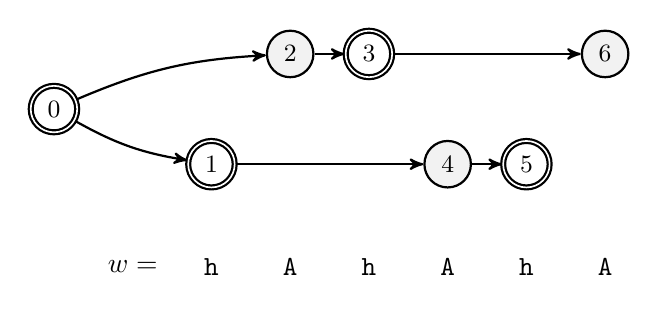
\begin{tikzpicture}[>=stealth', auto, semithick,
      honest/.style={circle,draw=black,thick,text=black,double,font=\small},
     malicious/.style={fill=gray!10,circle,draw=black,thick,text=black,font=\small}]
      \node at (0,-2) {$w =$};
    \node at (1,-2) {$\h$}; \node[honest] at (1,-.7) (b1) {$1$};
    \node at (2,-2) {$\A$}; \node[malicious] at (2,.7) (a1) {$2$};
    \node at (3,-2) {$\h$}; \node[honest] at (3,.7) (a2) {$3$};
    \node at (4,-2) {$\A$}; \node[malicious] at (4,-.7) (b2) {$4$};
    \node at (5,-2) {$\h$}; \node[honest] at (5,-.7) (b3) {$5$};
    \node at (6,-2) {$\A$}; \node[malicious] at (6,.7) (a3) {$6$};
      \node[honest] at (-1,0) (base) {$0$};
    \draw[thick,->] (base) to[bend left=10] (a1);
        \draw[thick,->] (a1) -- (a2);
        \draw[thick,->] (a2) -- (a3);
    \draw[thick,->] (base) to[bend right=10] (b1);
        \draw[thick,->] (b1) -- (b2);
        \draw[thick,->] (b2) -- (b3);
      \end{tikzpicture} 
    \caption{A balanced fork}
    \label{fig:balanced-mh}
  % \end{figure}
  \end{minipage}
  \hfill
  \begin{minipage}{0.45\textwidth}\centering

  % \begin{figure}[ht]
  %   \centering
    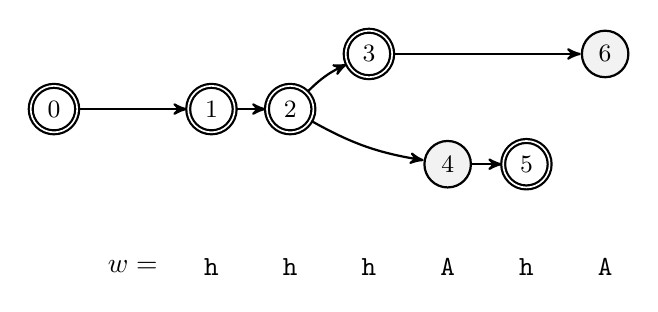
\begin{tikzpicture}[>=stealth', auto, semithick,
      honest/.style={circle,draw=black,thick,text=black,double,font=\small},
     malicious/.style={fill=gray!10,circle,draw=black,thick,text=black,font=\small}]
      \node at (0,-2) {$w =$};
    \node at (1,-2) {$\h$}; \node[honest] at (1,0) (ab1) {$1$};
    \node at (2,-2) {$\h$}; \node[honest] at (2,0) (ab2) {$2$};
    \node at (3,-2) {$\h$}; \node[honest] at (3,.7) (a3) {$3$};
    \node at (4,-2) {$\A$}; \node[malicious] at (4,-.7) (b3) {$4$};
    \node at (5,-2) {$\h$}; \node[honest] at (5,-.7) (b4) {$5$};
    \node at (6,-2) {$\A$}; \node[malicious] at (6,.7) (a4) {$6$};
      \node[honest] at (-1,0) (base) {$0$};
    \draw[thick,->] (base) -- (ab1);
    \draw[thick,->] (ab1) -- (ab2);
    \draw[thick,->] (ab2) to[bend left=10] (a3);
      \draw[thick,->] (a3) -- (a4);
    \draw[thick,->] (ab2) to[bend right=10] (b3);
      \draw[thick,->] (b3) -- (b4);
      \end{tikzpicture} 
    \caption{An $x$-balanced fork, where $x=\h\h$}
    \label{fig:x-balanced-mh}

  \end{minipage}
\end{figure}


% \paragraph{Balanced forks and settlement time.}
A fundamental question arising in typical blockchain settings is how
to determine \emph{settlement time}, the delay after which the
contents of a particular block of a blockchain can be considered
stable. The existence of a balanced fork is a precise indicator for
``settlement violations'' in this sense. Specifically, consider a
characteristic string $xy$ and a transaction appearing in a block
associated with the first slot of $y$ (that is, slot $|x| + 1$). One
clear violation of settlement at this point of the execution is the
existence of two chains---each of maximum length---which diverge
\emph{prior to $y$}; in particular, this indicates that there is an
$x$-balanced fork $F$ for $xy$. Let us record this observation below.\footnote{
  A balanced fork in~\cite{LinearConsistency} 
  had the property that 
  at least one maximum-length tine was adversarial. 
  But this is not true in our setting since we allow multiply honest slots.
}


\begin{observation}\label{obs:settlement-balanced-fork-mh}
  Let $s, k \in \NN$ be given and 
  let $w$ be a characteristic string. 
  Slot $s$ is not $k$-settled for the characteristic string $w$ 
  if 
  there exist a decomposition $w = xyz$, 
  where $|x| = s - 1$ and $|y| \geq k+1$, 
  and an $x$-balanced fork for $xy$. 
\end{observation}

In particular, to provide a rigorous $k$-slot settlement
guarantee---which is to say that the transaction can be considered
settled once $k$ slots have gone by---it suffices to show that with
overwhelming probability in choice of the characteristic string
determined by the leader election process (of a full execution of the
protocol), no such forks are possible. Specifically, if the protocol
runs for a total of $T$ time steps yielding the characteristics string
$w = xy$ (where $w \in \{0,1\}^T$ and the transaction of interest
appears in slot $|x| + 1$ as above) then it suffices to ensure that
there is no $x$-balanced fork for $x\hat{y}$, where $\hat{y}$ is an
arbitrary prefix of $y$ of length at least $k + 1$. 
% see Corollary~\ref{cor:main} in Section~\ref{sec:estimates}.  
Note that
for systems adopting the longest chain rule, this condition must
necessarily involve the \emph{entire future dynamics} of the
blockchain. We remark that our analysis below will in fact let us take
$T = \infty$.


% \paragraph{An alternative proof of Lemma~\ref{lemma:uvp-margin} via balanced forks.}
Let $w$ be a characteristic string. 
Writing $w = xy$, 
consider any tine-pair $(t_x, t_\rho)$ in a fork $F \Fork w$ so that 
$\reach_F(t_\rho) = \rho(F)$ and $t_x$ is $y$-disjoint with $t_\rho$.
Observe that if $\mu_x(y) < 0$ then $\reach_F(t_x) < 0$. 

% In a similar Fact 1 in~\cite{LinearConsistencySODA}, 
\begin{fact}\label{fact:margin-balance}
  Let $xy \in \{\h, \H, \A\}^*$ be a characteristic string. 
  There is no 
  $x$-balanced fork for $xy$ 
  if and only if 
  $\mu_x(y) < 0$.
\end{fact}
\begin{proof}[Proof sketch.]  
  If a fork $F \Fork xy$ 
  satisfies $\mu_x(F) \geq 0$, 
  it contains two $y$-disjoint tines $t_1, t_2$, 
  each with a non-negative reach, 
  so that $\min(\reach(t_1), \reach(t_2)) = \mu_x(F)$. 
  As $\reserve(t_i) \geq \gap(t_i)$ for $i \in \{1,2\}$, 
  we can extend these tines using only new adversarial vertices 
  so that both these extensions 
  have the maximum length 
  in the augmented fork. 
  Thus the augmented fork is $x$-balanced.

  On the other hand, if a fork $F \Fork xy$ is $x$-balanced, 
  there must be two $y$-disjoint 
  maximum-length tines $t_1, t_2 \in F$. 
  As the gap of a maximum-length tine is zero, 
  we must have $\reach(t_i) = \reserve(t_i) \geq 0$ 
  for $i \in \{1, 2\}$. 
  It follows that $\mu_x(y) \geq \mu_x(F) \geq \min_i \reach(t_i) \geq 0$.
\end{proof}

% Let us focus on proving Lemma~\ref{lemma:uvp-margin} 
% using the above fact. 
% Let $x\Prefix w$. 
% It is easy to see that 
% if the slot $s = |x| + 1$ has the UVP 
% then there can be no $x$-balanced fork for $xx'$ 
% where $xx' \PrefixEq w$;
% consequently, $\mu_x(x') < 0$. 
% On the other hand, if $s$ does not have the UVP 
% then there must be a prefix $xx' \PrefixEq w$ 
% and a fork $F \Fork xx'$ 
% containing two maximum-length (and hence viable) 
% tines $t_1, t_2$ 
% diverging prior to slot $s$. 
% Hence $F$ is $x$-balanced.
% \hfill\qed


\subsection{Relative margin 
to characterize 
the UVP}
Let $w$ be a characteristic string. 
Recall that in Theorem~\ref{thm:unique-honest}, 
we showed that whether a slot has the UVP in $w$ --- a 
structural property of the forks for $w$ --- is 
characterized by the ``Catalan-ness'' of the said slot. 
Below, we show that relative margin 
has the same expressive power 
as the Catalan slots 
in terms of characterizing the UVP. 


  
% \begin{definition}[Margin-critical slot]\label{def:margin-critical-slot}
%     Let $w \in \{\h,\H,\A\}^T$ be a characteristic string, 
%     $s \in [T]$ be a slot in $w$, 
%     and $x$ be a prefix of $w$ so that $|x| = s - 1$. 
%     Slot $s$ is called \emph{margin-critical} 
%     if, 
%     for all decompositions 
%     $w = xyz$ so that $|y| \geq 1$ and $|z| \geq 0$, 
%     we have $\mu_{x}(y) < 0$.
%     % for all decompositions $w = xyz$ so that $|x| < s, |xy| \geq s$.    
% \end{definition}
% Since $\mu_x(\varepsilon) \geq 0$ and $|y| \geq 1$ in the above definition, 
% it follows that a margin-critical slot (i.e., the first slot in $y$) must be honest.




% Below, we show that a margin-critical honest slot has the bottleneck property as well. 
\begin{lemma}\label{lemma:uvp-margin}
  Let $T \in \NN, w \in \{\h, \H, \A\}^T$, and 
  $s \in [T]$ so that $w_s = \h$. 
  Let $x = w_1 \ldots w_{s-1}$.
  Slot $s$ has the UVP in $w$ 
  if and only if 
  for every prefix $xy \PrefixEq w$, 
  $\mu_x(y) < 0$. 
  % A a uniquely honest slot is margin-critical 
  % if and only if 
  % it has the UVP. 
\end{lemma}


% \begin{corollary}\label{coro:catalan-margin-critical}
%   Let $w \in \{\h, \H, \A\}^T$ be a characteristic string 
%   and let $x \PrefixEq$ 
%   A uniquely honest slot in $w$ 
%   is Catalan 
%   if and only if 
%   % it is margin-critical. 
%   for every prefix $xy \PrefixEq w$, 
%   $\mu_x(y) < 0$. 
% \end{corollary}

\begin{proof}~
  % Recall from Theorem~\ref{thm:unique-honest} 
  % that a uniquely honest slot is Catalan in $w$ 
  % if and only if 
  % it has the UVP in $w$. 

  \begin{description}[font=\normalfont\itshape\space]
    \item[The $\Longleftarrow$ direction.]
      Suppose that 
      for every prefix $xy \PrefixEq w$ where $|y| \geq 1$, 
      we have $\mu_x(y) < 0$. 
      We wish to show that $s$ has the UVP in $w$.

      Let $F$ be any fork for $xy$ 
      and let 
      $t \in F, \ell(t) \leq s - 1$ be an honest tine. 
      Since it is disjoint with any tine in $F$ over the suffix $y$, 
      $\reach(t) < 0$ and, by Fact~\ref{fact:fork-structure-reach}, 
      $t$ does not have an adversarial extension $t' \in F, t \Prefix t'$ that is 
      viable at the onset of slot $|xy| + 1$. 
      Therefore, if a tine in $F$ 
      is viable at the onset of slot $|xy| + 1$, 
      it must contain an honest vertex with label at least $s$. 
      However, since an honest vertex builds only on top of a viable tine, 
      it follows that any viable tine must contain 
      the unique honest vertex with label $s$.

    \item[The $\Longrightarrow$ direction.]
      Suppose $s$ has the UVP in $w$.
      Let $k \in [s, T]$ be an integer and 
      write $w = xyz$ with $|xy| = k$. 
      (Note that $y_1 = w_s$.)
      We wish to show that $\mu_x(y) < 0$.

      Let $F$ be any fork for $xy$.
      % all tines in $F$ viable at the onset of 
      % % slot $|xy| + 1$ 
      % slot $|xy| + 1$ 
      % have, as their common prefix, 
      % {\color{blue}the unique honest tine} $\tau, \ell(\tau) = s$. 
      Since slot $s$ belongs to $y$, 
      $F$ cannot contain two tines 
      such that 
      \begin{enumerate*}[label=(\roman*)]
        \item both tines are viable at the onset of slot $|xy| + 1$ 
        and, at the same time, 
        \item disjoint over the length of $y$ 
        since they must contain the unique vertex with label $s$. 
      \end{enumerate*}
      % As any $x$-balanced fork for $xy$ requires two maximally long tines 
      % that are disjoint over $y$, 
      In particular, 
      $F$ cannot be $x$-balanced. 
      As $F$ was an arbitrary fork for $xy$, 
      no fork for $xy$ can be $x$-balanced for our choice of $k$.
      We use Fact~\ref{fact:margin-balance} 
      to conclude that 
      $\mu_x(y)$ must be negative.
      % Since our $k \in [s, T]$ is arbitrary, 
      % the above conclusion applies to 
      % all decompositions $w = xyz$ where $|x| = s - 1$ and $|xy| \geq s$.
      % Therefore, slot $s$ is margin-critical in $w$.

  \end{description}
\end{proof}









\subsection{An optimal online adversary against slot settlement}
\label{sec:opt-adversary}
Let $w$ be a characteristic string. 
For a fixed decomposition $w = xy$, 
there is an adversary\footnote{
  Specifically, 
  let $w' = xyb$ 
  where $b \in \{\h, \H, \A\}$. 
  This strategy recursively builds a closed fork $F \Fork xy$. 
  Then, upon encountering $b$, 
  it augments $F$ 
  by making zero, one, or two conservative extensions, as follows: 
  If $b = \A$, it does nothing. 
  If $b = \h$, it extends a zero-reach tine if possible; 
  otherwise,it extends a maximum-reach tine. 
  If $b = \H$, it extends a pair of tines that 
  witness $\mu_x(F)$. 
  By following the arguments in~\cite{LinearConsistencySODA}, 
  one can show that 
  if $\mu_x(F) = \mu_x(y)$ then 
  $\mu_x(F')$ is 
  at least as large as 
  the right-hand side in~\eqref{eq:mu-relative-recursive-mh}.   
} 
who builds a fork $F \Fork xy$ 
so that the $\mu_x(F)$ is 
at least as large as 
the right-hand side of~\eqref{eq:mu-relative-recursive-mh}. 
However, 
in light of Lemma~\ref{lemma:uvp-margin}, 
if an adversary wants to violate the settlement 
\emph{of all possible slots of $w$ at once}, 
% to show that the lowerbound is satisfied 
% \emph{simultaneously} 
% for all decompositions $w = xy$, 
% one has to do more work.
he needs to produce a fork $F$ for $w$ 
so that $\mu_x(F) \geq 0$ 
for every prefix $x \PrefixEq w$. 
In Figure~\ref{fig:adv-opt-mh}, 
we describe a strategy $\Adversary^*$ 
which does even better: 
it produces a fork $F$ so that $\mu_x(F) = \mu_x(y)$ 
for every prefix $x \PrefixEq w$. 


$\Adversary^*$ builds a fork for $w = w_1 \ldots w_{n+1}$ 
in an online fashion, i.e., 
it scans $w$ once, from left to right, 
maintains a fork $F_n$ after scanning 
the first $n$ symbols, 
and augments $F_n$ by conservatively extending 
zero-reach tine(s) using label $n + 1$.
Specifically, if $w_{n+1} = \A$, $\Adversary^*$ does nothing. 
If $w_{n+1} = \h$, it (obviously) makes a single extension. 
Now suppose $w_{n+1} = \H$. 
It still makes a single extension
if either $F_n$ contains exactly one zero-reach tine 
or $F_n$'s reach is positive. 
Otherwise, 
if $\rho(F_n) = 0$ 
and there are at least two zero-reach tines in $F_n$, 
$\Adversary^*$ extends two zero-reach tines 
that diverge earliest in $F_n$.



\begin{figure}[!h]
  \begin{center}
    \fbox{
      \begin{minipage}{.9 \textwidth}
        \begin{center}
          \textbf{The strategy $\Adversary^*$}
        \end{center}
        Let $n$ be a non-negative integer, 
        $w \in \{\h, \H, \A\}^n$, 
        and $w_{n + 1} \in \{\h, \H, \A\}$. 
        If $n = 0$, set $F_0 \Fork \varepsilon$ as 
        the trivial fork comprising a single vertex. 
        Otherwise, 
        let $F_n$ be the closed fork 
        built recursively by $\Adversary^*$ for the string $w$. 
        If $w_{n + 1} = \A$, 
        output $F_n$ (as a fork for $w w_{n+1}$). 
        Otherwise, 
        let $Z$ and $R$ be the set of zero-reach tines 
        and maximum-reach tines in $F_n$, respectively.

        \begin{enumerate}
          \item 
          Identify a set $S$ as follows: 
          If $|Z| = 1$ then set $S = Z$. 
          Otherwise, 
          let $r_1 \in R, z_1 \in Z$ be two tines so that 
          $\ell(r_1 \Intersect z_1) = 
          \min\{ \ell(r \Intersect z) :  r \in R, z \in Z \}$ 
          and set  
          \[
          S = \begin{cases}
            \{z_1\} & \text{
              if $w_{n + 1} = \h$ 
              or $\rho(F_n) \geq 1$ 
              % or for all prefix $x \Prefix w$, $\mu_x(F_n) < 0$}
              % or $|Z| = 1$
              }\,, \\
            \{z_1, r_1\} & \text{otherwise}\,.
          \end{cases}
          \]

          \item
          Conservatively extend 
          each tine in $S$ 
          using label $n + 1$. 
          Let $F_{n + 1} \Fork w w_{n+1}$ 
          be the new closed fork. 
          Output $F_{n+1}$.
        \end{enumerate}
      \end{minipage}
    }
  \end{center}
  \caption{Optimal online adversary $\Adversary^*$}
  \label{fig:adv-opt-mh}
\end{figure}






\begin{definition}[Canonical fork]
  A \emph{canonical fork} for $w \in \{\h, \H, \A\}^*$ 
  is a closed fork $F \Fork w$ so that 
  $\rho(F) = \rho(w)$ 
  and, for all prefixes $x \Prefix w$, $\mu_x(F) = \mu_x(y)$. 
  If $|w| = 0$, $F$ is 
  the unique fork with a single (honest) vertex and no edge. 
  % Let $w_1 \ldots w_T \in \{0,1\}^T$. 
  % For $n = 0, 1, \ldots, T$, a \emph{canonical fork $F_n$ for $w = w_1\ldots w_n$} 
  % is inductively defined as follows. 
  % If $n = 0$ then $F_0$ is the trivial fork for the empty string; 
  % it consists of a single (honest) vertex and no edge. 
  % If $n \geq 1$, the following holds: 
  % $F_n$ is a closed fork so that $F_{n-1} \ForkPrefix F_n$. 
  % $F_n$ contains an honest tine $\tau_\rho$ so that 
  % $\reach(\tau_\rho) = \rho(F_n) = \rho(w)$. 
  % For every decomposition $w = xy, x \Prefix w$, 
  % % $\mu_x(F_n) = \mu_x(y)$ and, in addition, 
  % $F_n$ contains two honest tines $\tau_x, \tau_{\rho x}$ 
  % so that the tine-pair $(\tau_{\rho x}, \tau_x)$ witnesses $\mu_x(F_n) = \mu_x(y)$. 
  % The (possibly non-distinct) designated tines $\tau_\rho, \tau_{\rho x}, \tau_x, x \Prefix w$ 
  % are called the \emph{witness tines}. 
  % For the sake of completeness, define $\tau_w = \tau_{\rho w} = \tau_\rho$.
\end{definition}

It is not obvious whether a canonical fork always exists 
or whether it can be found algorithmically. 
The theorem below gives us the assurance:


\begin{theorem}\label{thm:opt-adversary-canonical}
  Let $w \in \{\h, \H, \A\}^*$. 
  The strategy $\Adversary^*$ in Figure~\ref{fig:adv-opt-mh}
  outputs a canonical fork for $w$.  
\end{theorem}
That is, for every characteristic string $w$ 
there is a fork $F \Fork w$ so that 
for every prefix $x \PrefixEq w$, $\mu_x(F) = \mu_x(y)$. 
Note that if one's objective is to create a fork 
which contains many early-diverging tine-pairs (that witness large relative margins), 
a canonical fork is the best one can hope for. 
This is why $\Adversary^*$ is called an \emph{optimal} online adversary. 
The proof of Theorem~\ref{thm:opt-adversary-canonical} 
is given in Section~\ref{sec:margin-proof}.







\subsection{An algorithm to compute exact settlement probabilities}
\label{sec:exact-prob}
Let $m, k \in \NN$  and $\epsilon \in (0,1]$. 
Let $w$ be a characteristic string of length $T = m + k$ such that 
the bits of $w$ are i.i.d.\ Bernoulli with expectation $\alpha = (1 - \epsilon)/2$. 
Write $w$ as $w = xy$ where $|x| = m, |y| = k$.
% where 
% each bit is independent with $\Pr[w_i = 1] = \alpha$.
The recursive definition of relative margin (cf. Lemma~\ref{lem:relative-margin}) 
implies an algorithm for computing the probability
$\Pr[\mu_x(y) \geq 0]$ in time $\Poly(m, k)$. In typical
circumstances, however, it is more interesting to establish an
explicit upper bound on $\Pr[\mu_x(y) \geq 0]$ where
$|x| \rightarrow \infty$; this corresponds to the case where the
distribution of the initial reach $\rho(x)$ is the dominant distribution
$\StationaryRho$ in Lemma~\ref{lemma:rho-stationary}. 
Due to dominance, $\StationaryRho(m)$ serves as an
upper bound on $\rho(x)$ for any finite $m = |x|$. 
For this purpose, one can implicitly
maintain a sequence of matrices $\left( M_t \right)$ for $t = 0, 1, 2, \cdots, k$
such that $M_0(r, r) = \StationaryRho(r)$ for all $0 \leq r \leq 2k$ and
the invariant
\[
  M_t(r, s) = \Pr_{y \sim \mathcal{B}(t, \alpha)}[\rho(xy) = r \text{ and }
  \mu_x(y) = s ]
\]
is satisfied for every integer $t \in [1, k]$,
$r \in [0, 2k]$, and $s \in [-2k, 2k]$. 
Here, $M(i,j)$ denotes the entry at the $i$th row and $j$th column of the matrix $M$.
%The matrix $M_0$ corresponds to the reach and margin after any prefix $x$. 
Observe that $M_t(r,s)$ can be computed solely from the neighboring cells of $M_{t-1}$, that is, 
from the values $M_{t-1}(r\pm 1, s \pm 1)$. 
Of course, only the transitions approved by the recursions in 
Lemma~\ref{lem:margin} and Lemma~\ref{lem:relative-margin} should be considered.

Finally, one can compute $\Pr[\mu_x(y) \geq 0]$ by summing $M_k(r,s)$ for
$r, s \geq 0$. Table~\ref{table:exact-probs} contains these
probabilities where $\alpha$ ranges from $0.05$ to $0.40$ and $k$
ranges from $50$ to $1000$. 
In addition, Figure~\ref{fig:exact-probs} shows the base-$10$ logarithm of
these probabilities. The
points corresponding to a fixed $\alpha$ appear to form a straight
line. This means the probability decays exponentially in $k$, or equivalently, that the exponent 
depends linearly on $k$, 
as stipulated by Bound~\ref{bound:analytic}. 

A \texttt{C++} implementation of the above algorithm is publicly available 
at: \\
\href{https://github.com/saad0105050/forkable-strings-code}{https://github.com/saad0105050/forkable-strings-code}~\cite{PrForkableCode}.



\begin{figure}[h!]

\centering
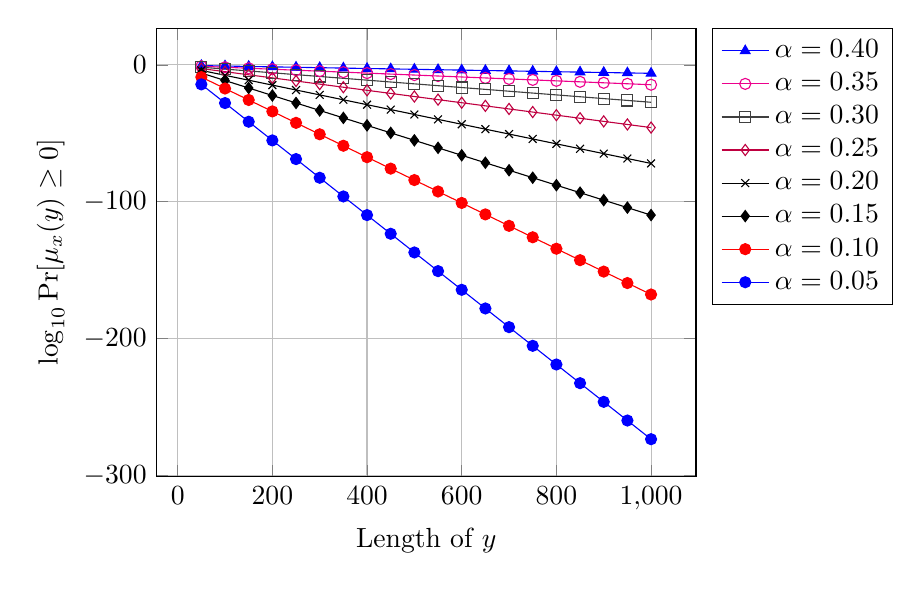
\begin{tikzpicture}
  \begin{axis}[
    xlabel=Length of $y$,
    ylabel=${\log_{10} \Pr[ \mu_x(y) \geq 0 ]}$,
    legend pos = outer north east,
    grid = both
    %,height = 7cm
    ]


    %============= \alpha = 0.40    
      \addplot[color=blue,mark=triangle*] coordinates {
    (50, -0.534881009996625)
    (100, -0.861843437303938)
    (150, -1.17110438398993)
    (200, -1.47350880258986)
    (250, -1.77251864117173)
    (300, -2.06962896433787)
    (350, -2.36559449154758)
    (400, -2.66083495643829)
    (450, -2.95559969289654)
    (500, -3.25004400806221)
    (550, -3.54426813580273)
    (600, -3.83833855715903)
    (650, -4.1323003235163)
    (700, -4.42618449355664)
    (750, -4.72001278023346)
    (800, -5.01380053810684)
    (850, -5.30755872931896)
    (900, -5.60129524293208)
    (950, -5.89501579493968)
    (1000, -6.18872455077118)


      };
      
    %============= \alpha = 0.35    
      \addplot[color=magenta,mark=o] coordinates {
    (50, -1.02877436841824)
    (100, -1.76405795532126)
    (150, -2.48156081504761)
    (200, -3.19351655688251)
    (250, -3.90324719739329)
    (300, -4.6119732073238)
    (350, -5.32021396523135)
    (400, -6.0282101484992)
    (450, -6.73607948155516)
    (500, -7.44388168223398)
    (550, -8.15164782799613)
    (600, -8.85939439475358)
    (650, -9.56713023906372)
    (700, -10.2748601722391)
    (750, -10.9825868295165)
    (800, -11.6903116636224)
    (850, -12.3980354795589)
    (900, -13.1057587252749)
    (950, -13.8134816508858)
    (1000, -14.521204396449)  


      };

    %============= \alpha = 0.30    
        \addplot[color=darkgray,mark=square] coordinates {
    (50, -1.73119438208806)
    (100, -3.09673279902966)
    (150, -4.44780375955355)
    (200, -5.79553003490465)
    (250, -7.14227457376805)
    (300, -8.48869966525932)
    (350, -9.83501495946096)
    (400, -11.1812912676285)
    (450, -12.5275534426098)
    (500, -13.873810422115)
    (550, -15.2200654730463)
    (600, -16.5663198030557)
    (650, -17.9125738621863)
    (700, -19.258827819142)
    (750, -20.6050817374433)
    (800, -21.9513356410858)
    (850, -23.2975895391646)
    (900, -24.6438434351249)
    (950, -25.9900973302771)
    (1000, -27.3363512251228)  


      };



    %============= \alpha = 0.25    
      \addplot[color=purple,mark=diamond] coordinates {
    (50, -2.7068067143968)
    (100, -4.98669572210932)
    (150, -7.25681899248793)
    (200, -9.52547099796917)
    (250, -11.793848036259)
    (300, -14.0621691284583)
    (350, -16.3304783495448)
    (400, -18.5987849921223)
    (450, -20.8670910667017)
    (500, -23.1353970150404)
    (550, -25.4037029351594)
    (600, -27.6720088489442)
    (650, -29.9403147613032)
    (700, -32.2086206733433)
    (750, -34.4769265853085)
    (800, -36.7452324972576)
    (850, -39.0135384092045)
    (900, -41.281844321149)
    (950, -43.5501502330935)
    (1000, -45.8184561450381)


      };


          
    %============= \alpha = 0.    
      \addplot[color=black,mark=x] coordinates {
    (50, -4.06125884952046)
    (100, -7.64248504871986)
    (150, -11.2184152058828)
    (200, -14.7939108371324)
    (250, -18.3693634087138)
    (300, -21.9448114175389)
    (350, -25.520258928049)
    (400, -29.095706383289)
    (450, -32.6711538323473)
    (500, -36.2466012807114)
    (550, -39.822048728996)
    (600, -43.3974961772738)
    (650, -46.9729436255496)
    (700, -50.5483910738248)
    (750, -54.1238385221004)
    (800, -57.6992859703754)
    (850, -61.2747334186509)
    (900, -64.8501808669272)
    (950, -68.4256283152027)
    (1000, -72.0010757634778)




      };
      
    %============= \alpha = 0.15    
      \addplot[color=black,mark=diamond*] coordinates {
    (50, -5.99101535930985)
    (100, -11.4538646368115)
    (150, -16.9145865673508)
    (200, -22.3752357117723)
    (250, -27.8358819361379)
    (300, -33.2965280374903)
    (350, -38.7571741335604)
    (400, -44.2178202294009)
    (450, -49.6784663252318)
    (500, -55.1391124210625)
    (550, -60.5997585168932)
    (600, -66.0604046127235)
    (650, -71.5210507085538)
    (700, -76.9816968043839)
    (750, -82.4423429002152)
    (800, -87.9029889960452)
    (850, -93.3636350918761)
    (900, -98.8242811877078)
    (950, -104.284927283538)
    (1000, -109.745573379367)


    };


    %============= \alpha = 0.10    
      \addplot[color=red,mark=*] coordinates {
    (50, -8.93400016060089)
    (100, -17.292337808078)
    (150, -25.6501551609344)
    (200, -34.007967886374)
    (250, -42.3657805652942)
    (300, -50.7235932437328)
    (350, -59.0814059221663)
    (400, -67.4392186006004)
    (450, -75.7970312790341)
    (500, -84.1548439574669)
    (550, -92.5126566359009)
    (600, -100.870469314334)
    (650, -109.228281992768)
    (700, -117.586094671201)
    (750, -125.943907349634)
    (800, -134.301720028069)
    (850, -142.659532706502)
    (900, -151.017345384936)
    (950, -159.375158063369)
    (1000, -167.732970741802)



    };
    %============= \alpha = 0.05    
      \addplot[color=blue,mark=*] coordinates {
    (50, -14.2699842004544)
    (100, -27.9093384792564)
    (150, -41.5486518624197)
    (200, -55.1879652167995)
    (250, -68.8272785711567)
    (300, -82.4665919255127)
    (350, -96.10590527987)
    (400, -109.745218634226)
    (450, -123.384531988584)
    (500, -137.023845342941)
    (550, -150.663158697297)
    (600, -164.302472051655)
    (650, -177.94178540601)
    (700, -191.581098760368)
    (750, -205.220412114725)
    (800, -218.859725469083)
    (850, -232.499038823439)
    (900, -246.138352177796)
    (950, -259.777665532154)
    (1000, -273.41697888651)

 
  };
  \legend{
  $\alpha = 0.40$, $\alpha = 0.35$, 
   $\alpha = 0.30$,$\alpha = 0.25$, $\alpha = 0.20$, 
   $\alpha = 0.15$,$\alpha = 0.10$,  $\alpha = 0.05$
  }
  \end{axis}%
\end{tikzpicture}%
\caption{The probabilities from Table~\ref{table:exact-probs}  
drawn in the base-$10$ logarithmic scale. 
}
\label{fig:exact-probs}
\end{figure}

%%%%% If dissertation, display table in landscape mode
\iftoggle{Dissertation}{
  \begin{landscape}
}

\begin{table}[h]
	\centering
	\caption{
		Exact probabilities $\Pr[\mu_x(y) \geq 0]$ where 
		the bits of the characteristic string $xy$ are i.i.d.\ Bernoulli with expectation $\alpha$. 
		Each row of the table corresponds to a different $k = |y|$.
	} 
	\label{table:exact-probs}


	\begin{tabular}{|l||l|l|l|l|l|l|l|l|}
	\hline
	\multicolumn{1}{|c||}{\multirow{2}{*}{$k$}} & \multicolumn{8}{c|}{$\alpha$}                                             \\ \cline{2-9} 
	\multicolumn{1}{|c||}{}                   & 0.05     & 0.10      & 0.15     & 0.20      & 0.25     & 0.30      & 0.35     & 0.40      \\ 
	\hhline{|=#=|=|=|=|=|=|=|=|}
	50   & 5.37E-15  & 1.16E-09  & 1.02E-06  & 8.68E-05 & 1.96E-03 & 1.86E-02 & 9.36E-02 & 2.92E-01 \\ \hline
	100  & 1.23E-28  & 5.10E-18  & 3.52E-12  & 2.28E-08 & 1.03E-05 & 8.00E-04 & 1.72E-02 & 1.37E-01 \\ \hline
	150  & 2.83E-42  & 2.24E-26  & 1.22E-17  & 6.05E-12 & 5.54E-08 & 3.57E-05 & 3.30E-03 & 6.74E-02 \\ \hline
	200  & 6.49E-56  & 9.82E-35  & 4.21E-23  & 1.61E-15 & 2.98E-10 & 1.60E-06 & 6.40E-04 & 3.36E-02 \\ \hline
	250  & 1.49E-69  & 4.31E-43  & 1.46E-28  & 4.27E-19 & 1.61E-12 & 7.21E-08 & 1.25E-04 & 1.69E-02 \\ \hline
	300  & 3.42E-83  & 1.89E-51  & 5.05E-34  & 1.14E-22 & 8.67E-15 & 3.25E-09 & 2.44E-05 & 8.52E-03 \\ \hline
	350  & 7.84E-97  & 8.29E-60  & 1.75E-39  & 3.02E-26 & 4.67E-17 & 1.46E-10 & 4.78E-06 & 4.31E-03 \\ \hline
	400  & 1.80E-110 & 3.64E-68  & 6.06E-45  & 8.02E-30 & 2.52E-19 & 6.59E-12 & 9.37E-07 & 2.18E-03 \\ \hline
	450  & 4.13E-124 & 1.60E-76  & 2.10E-50  & 2.13E-33 & 1.36E-21 & 2.97E-13 & 1.84E-07 & 1.11E-03 \\ \hline
	500  & 9.47E-138 & 7.00E-85  & 7.26E-56  & 5.67E-37 & 7.32E-24 & 1.34E-14 & 3.60E-08 & 5.62E-04 \\ \hline
	550  & 2.17E-151 & 3.07E-93  & 2.51E-61  & 1.51E-40 & 3.95E-26 & 6.02E-16 & 7.05E-09 & 2.86E-04 \\ \hline
	600  & 4.98E-165 & 1.35E-101 & 8.70E-67  & 4.00E-44 & 2.13E-28 & 2.71E-17 & 1.38E-09 & 1.45E-04 \\ \hline
	650  & 1.14E-178 & 5.91E-110 & 3.01E-72  & 1.06E-47 & 1.15E-30 & 1.22E-18 & 2.71E-10 & 7.37E-05 \\ \hline
	700  & 2.62E-192 & 2.59E-118 & 1.04E-77  & 2.83E-51 & 6.19E-33 & 5.51E-20 & 5.31E-11 & 3.75E-05 \\ \hline
	750  & 6.02E-206 & 1.14E-126 & 3.61E-83  & 7.52E-55 & 3.33E-35 & 2.48E-21 & 1.04E-11 & 1.91E-05 \\ \hline
	800  & 1.38E-219 & 4.99E-135 & 1.25E-88  & 2.00E-58 & 1.80E-37 & 1.12E-22 & 2.04E-12 & 9.69E-06 \\ \hline
	850  & 3.17E-233 & 2.19E-143 & 4.33E-94  & 5.31E-62 & 9.69E-40 & 5.04E-24 & 4.00E-13 & 4.93E-06 \\ \hline
	900  & 7.27E-247 & 9.61E-152 & 1.50E-99  & 1.41E-65 & 5.23E-42 & 2.27E-25 & 7.84E-14 & 2.50E-06 \\ \hline
	950  & 1.67E-260 & 4.22E-160 & 5.19E-105 & 3.75E-69 & 2.82E-44 & 1.02E-26 & 1.54E-14 & 1.27E-06 \\ \hline
	1000 & 3.83E-274 & 1.85E-168 & 1.80E-110 & 9.98E-73 & 1.52E-46 & 4.61E-28 & 3.01E-15 & 6.48E-07 \\ \hline
	\end{tabular}

\end{table}
%%%%% If dissertation, display table in landscape mode
\iftoggle{Dissertation}{
  \end{landscape}
}



%%% Local Variables:
%%% mode: latex
%%% TeX-master: "main"
%%% End:


\section{Proofs of Theorem~\ref{thm:relative-margin} and Theorem~\ref{thm:opt-adversary-canonical}}
\label{sec:margin-proof}


The proof of Theorem~\ref{thm:relative-margin} is presented in two parts. 
Let $w \in \{\h, \H, \A\}^*$.
First, for a given decomposition $w = xy$, 
 % and $b \in \{\h, \H\}$, 
we prove an upper bound on $\mu_x(y)$. 
Next, 
considering the fork $F \Fork w$ built by the strategy $Adversary^*$ 
(see Figure~\ref{fig:adv-opt-mh}), 
we show that 
for every decomposition $w = xy$, 
$\mu_x(F)$ is at least as large as the upper bound proven in the first part; 
thus $F$ is canonical. 

As a warm-up, we start with the following claim.

\begin{claim}\label{claim:rho-mu-A}
  $\rho(\varepsilon) = 0$. 
  For any $x, y \in \{\h, \H, \A\}^*$, 
  $\mu_x(\varepsilon) = \rho(x)$, 
  $\rho(xy\A) = \rho(xy) + 1$, 
  and $\mu_x(y\A) = \mu_x(y) + 1$.
\end{claim}
\begin{proof}
  The only possible fork for the empty string $\varepsilon$ 
  contains a single honest vertex 
  with reserve and gap both zero; 
  hence $\rho(\varepsilon) = 0$.

  Let $F$ be a closed fork for the characteristic string $xy$. 
  Let $t_\rho, t_x \in F$ be the two tines that witness $\mu_x(F)$, 
  i.e., $\reach(t_\rho) = \rho(F), \reach_F(t_x) = \mu_x(F)$, 
  and $t_\rho, t_x$ are disjoint over $y$. 
  % Let $\hat{t}$ be the longest tine in $F$.


  In the base case, where $y=\varepsilon$, 
  observe that any two tines of $F$ 
  are disjoint over $y$. 
  Moreover, a single tine $t \in F$ 
  is disjoint with itself over the empty suffix $\varepsilon$. 
  Therefore, the relative margin $\mu_x(\varepsilon)$ must be at least $\rho(x)$. 
  As $\mu_x(F)$ can be no more than $\rho(x)$, it follows that 
  $\mu_x(\varepsilon) = \rho(x)$.


  Now consider a pair of closed forks $F\vdash xy$ and $F'\vdash xy\A$ 
  such that $F \fprefix F'$ and $x,y\in\{\h, \H, \A\}^*$. 
  We must have $F' = F$ since $F'$ is closed. 
  In addition, for any tine $t \in F$, 
  $\reach_{F'}(t) = \reach_F(t) + 1$ 
  since the reserve has increased by one 
  but the gap is unchanged 
  (as no new tine is added). Therefore, 
  $\rho(xy\A) = \rho(xy) + 1$ and 
  $\mu_x(y\A) = \mu_x(y)+1$.
\end{proof}


\section{An upper bound on relative margin}

\begin{proposition}\label{prop:mu-upperbound}
  Let $w,x, y \in \{\h, \H, \A\}^*$ 
  and $b \in \{\h, \H\}$, 
  Then 
  \begin{equation}
    \rho(xyb) \leq \begin{cases}
      0 & \text{if $\rho(xy) = 0$}\,, \\
      \rho(xy) - 1 & \text{otherwise.}
    \end{cases}
    \label{eq:rho-upperbound}
  \end{equation}
  Furthermore,
  \begin{equation}
    \mu_x(yb) \leq \begin{cases}
      0 & \text{if $\rho(xy) > \mu_x(y)=0$}\,, \\
      0 & \text{if $\rho(xy) = \mu_x(y) = 0$ and $b = \H$}\,, \\
      \mu_x(y)-1 & \text{otherwise.}
    \end{cases}
    \label{eq:mu-upperbound}
  \end{equation}
\end{proposition}
\begin{proof}
  Suppose $F'\vdash xyb$ is a closed fork such that 
  $\rho(xyb)=\rho(F')$ and $\mu_x(yb)=\mu_x(F')$. 
  Let $t_\rho, t_x \in F'$ be a pair of $y$-disjoint tines such that $\reach_{F'}(t_\rho)=\rho(F')$ and $\reach_{F'}(t_x)=\mu_x(F')$. 
  (If there are multiple candidates for $t_\rho$ or $t_x$, 
  select the one with the smallest $\leq_\pi$ rank.)
  Let $F\vdash xy$ be the unique closed fork such that $F\fprefix F'$.  
  Note that while $F'$ is obtained from one or more extensions 
  of $F$-tines, 
  these extensions are not necessarily conservative. 
  Recall that $\reach_{F'}(t) \leq 0$ for any tine $t \in F', \ell(t) = |xy| + 1$.

  \Paragraph{Proving ~\eqref{eq:rho-upperbound}.} 
  Let $A$ be the set of all $F'$-tines with label $|xy| + 1$.
  Let $\sigma \in A$ be the first tine in the $\leq_\pi$ ordering so that $\reach(\sigma) = \max_{t \in A}\{\reach_{F'}(t)\}$.
  By Proposition~\ref{prop:reach-fork-ext-mh}, 
  $\reach_{F'}(\sigma) \leq 0$ and, 
  in addition, for any $t \in F$, 
  $\reach_{F'}(t) \leq \reach_F(t) - 1$.   
  Let $\hat{t}$ be the maximum-reach tine in $F$ 
  with the smallest $\leq_\pi$ rank.

  If $\rho(F) = 0$ then 
  $\reach_{F'}(t) < 0$ for all $t \in F$. 
  Hence $t_\rho = \sigma$ and, consequently, 
  $\rho(xyb) \leq 0$. 
  If $\rho(F) \geq 2$ then $t_\rho \in F$
  % $\reach_{F'}(\hat{t}) \geq 1$ but $\reach_{F'}(\sigma) \leq 0$; 
  % thus $t_\rho = \hat{t}$ 
  and, therefore, 
  $\rho(xyb) = \reach_{F'}(t_\rho) \leq \rho(F) - 1 \leq \rho(xy) - 1$. 
  If $\rho(F) = 1$ and $t_\rho \in F$ then, 
  as before, 
  $\rho(xyb) = \reach_{F'}(\hat{t}) = \reach_{F}(\hat{t}) - 1 = \rho(F) - 1 \leq \rho(xy) - 1$.
  If $\rho(F) = 1$ and $t_\rho \not \in F$ then, as we have seen before, 
  $\rho(xyb) = \reach_{F'}(\sigma) \leq 0 = \rho(F) - 1\leq \rho(xy) - 1$.
  Thus we have proved~\eqref{eq:rho-upperbound}.


  \Paragraph{Proving ~\eqref{eq:mu-upperbound}.} 
  If $\ell(t_\rho) = |xy| + 1$ then we are done: 
  by our preceding argument, $\reach_{F'}(t_\rho) \leq 0$. 
  On the other hand, 
  Note that $t_\rho \not \in F$ since, by Proposition~\ref{prop:reach-fork-ext-mh}, reach of any $F$ tine can only decrease
  $t_\rho$ must have been an extension of a maximum-reach $F$-tine.

  \Paragraph{Case 1: $\rho(xy)>0$ and $\mu_x(y)=0$.} 
    We wish to show that $\mu_x(yb) \leq 0$.
    Suppose (toward a contradiction) that $\mu_x(yb) > 0$. 
    Then neither $t_\rho$ nor $t_x$ is a conservative extension because, as we proved in Claim ~\ref{claim:ex-mh}, conservative extensions have reach zero. This means that $t_\rho$ and $t_x$ existed in $F$, and their $F$-reach was strictly greater than their $F'$-reach (by Claim ~\ref{claim:nex-mh}). 
    Because $t_\rho$ and $t_x$ 
    % have been implicitly 
    are 
    disjoint over $y0$, they must also be disjoint over $y$; therefore, $\mu_x(F)$ must be at least $\min(\reach_F(t_\rho),\reach_F(t_x))$. 
    It follows that 
    $0 
    = \mu_x(y) 
    \geq \min(\reach_F(t_\rho),\reach_F(t_x))
    > \min(\reach_{F'}(t_\rho),\reach_{F'}(t_x))
    = \mu_x(F') = \mu_x(yb)
    $. 
    The last term is strictly positive by assumption and hence, a contradiction ensues.

  % \Paragraph{Case 2: $\rho(xy)=0$.}
  \Paragraph{Case 2: $\rho(xy)=0$.}
    We wish to show that 
    \begin{enumerate*}[label=(\textit{\roman*})]
      \item $\mu_x(yb) \leq 0$ if $b = \H$ and $\mu_x(y) = 0$, and 
      \item $\mu_x(yb) \leq \mu_x(y) - 1$ otherwise.
    \end{enumerate*}
    First, we claim that $t_\rho$ must arise from an extension. 
    Suppose, toward a contradiction, that $t_\rho$ is not an extension, 
    i.e., $t_\rho \in F$. 
    The fact that $t_\rho$ achieves the maximum reach in $F'$ 
    implies that 
    $t_\rho$ has a non-negative reach 
    since the longest honest tine always achieves reach zero. 
    Furthermore, 
    Claim ~\ref{claim:nex-mh} states that 
    all $F$-tines see their reach decrease. 
    Therefore, $t_\rho \in F$ must have had a strictly positive reach. 
    But this contradicts the central assumption of the case, i.e., 
    that $\rho(xy)=0$. 
    Therefore, we conclude that $t_\rho \in F' \setminus F$.

    Let $s \in F$ be the tine-prefix of $t_\rho \in F'$ so that 
    $t_\rho$ is an extension of $s$. 
    % Since $\reach_{F'}(t_\rho) = \rho(xy0) = 0$ by~\eqref{eq:rho-recursive-mh}, 
    Observe that $\reach_F(s)$ must be non-negative since 
    otherwise, $s$ could not have been extended. 
    In fact, our assumption $\rho(xy)=0$ implies that 
    $\reach_F(s) = 0$. 
    In addition, since $t_x$ and $t_\rho$ are disjoint over $yb$, 
    so are $t_x$ and $s$. 
    \begin{description}[font=\normalfont\itshape\space]
      % \item[If $t_x \in F$,] 
      \item[If $b = \h$,] 
      $t_\rho$ is the only extension in $F'$ and hence 
      $t_x$ must be in $F$. 
      Consequently, \\      
      $\min( \reach_F(s),\reach_F(t_x) ) \leq \mu_x(y)$. 
      Because $\reach_F(s)=0$ and $\reach_F(t_x) \leq \rho(xy)=0$, it follows that $\reach_F(t_x) \leq \mu_x(y)$. 
      Finally, since $t_x \in F$, 
      Claim ~\ref{claim:nex-mh} tells us that 
      $\reach_{F'}(t_x) < \reach_F(t_x)$. 
      Taken together, these two inequalities show that 
      $\mu_x(yb) = \reach_{F'}(t_x) < \reach_F(t_x) \leq \mu_x(y)$. 
      The last inequality follows since $s$ and $t_x$ are disjoint over $y$ and $\reach_F(s) = 0 = \rho(xy)$. 
      We conclude that $\mu_x(yb) \leq \mu_x(y) - 1$.

      \item[If $b = \H$ and $\mu_x(y) < 0$,] 
      % $F$ cannot contain a single maximum-reach tine and its
      we claim that $t_x \in F$. 
      To see why, note that as $t_x$ is $yb$-disjoint with $t_\rho$, 
      it must extend some $F$-tine $t$ that is $y$-disjoint with $t_\rho$. 
      However, as $\mu_x(y) < 0$, $t$ must have negative reach and hence cannot be extended into $t_x$; this is a contradiction. 
      Therefore, $t_x \in F$ and we can apply the argument in the ``$b = \h$'' case above 
      to conclude that $\mu_x(yb) \leq \mu_x(y) - 1$.

      \item[If $b = \H$ and $\mu_x(y) = 0$,] 
      then there are two alternatives depending on 
      whether $t_x$ is an extension. 
      If $t_x$ is not an extension, we can apply the argument in the ``$b = \h$'' case above and conclude that 
      $\mu_x(yb) \leq \mu_x(y) - 1 = -1$.
      On the other hand, if $t_x \not\in F$, 
      both $t_x$ and $t_\rho$ are extensions and, 
      by Proposition~\ref{prop:reach-fork-ext-mh}, 
      $\max(\reach_{F'}(t_x), \reach_{F'}(t_\rho) ) \leq 0$. 
      In addition, Proposition~\ref{prop:reach-fork-ext-mh} states that for all $t \in F$, 
      $\reach_{F'}(t) < \reach_{F}(t) \leq \rho(xy) = 0$. 
      We conclude that $\mu_x(yb) \leq 0$.

    \end{description}



  \Paragraph{Case 3: $\rho(xy)>0$ and $\mu_x(y)\neq0$.}
    We wish to show that $\mu_x(yb) \leq \mu_x(y) - 1$ 
    or, equivalently, that $\mu_x(yb) < \mu_x(y)$. 
    % Note that by~\ref{eq:rho-recursive-mh}, 
    % $\rho(xy0) = \rho(xy) - 1 \geq 0$.
    We will break this case into two sub-cases. 
    \begin{description}[font=\normalfont\itshape\space]
      \item[If both $t_\rho, t_x \in F$,] 
      then $\mu_x(yb) = \reach_{F'}(t_x) < \reach_{F}(t_x) \leq \mu_x(y)$. 
      Here, the first inequality follows from Proposition~\ref{prop:reach-fork-ext-mh} 
      and the second inequality follows from the fact that 
      $t_x, t_\rho$ is $y$-disjoint and 
      $\reach(t_x)$ is at most $\reach(t_\rho)$ by design.

      \item[Otherwise,] 
      at least one of $t_x, t_\rho$ arose from an extension. 
      Since $\reach_{F'}(t_x) \leq \reach_{F'}(t_\rho)$ by design, 
      it follows that $\reach_{F'}(t_x) \leq 0$ 
      as the reach of an extension is at most zero.
      If $\mu_x(y) > 0$ then we are done: $\mu_x(yb) \leq 0 < \mu_x(y)$.  
      On the other hand, suppose $\mu_x(y) < 0$. 
      Recall the tine $s$ mentioned before.
      As $t_x$ is $y$-disjoint with $s$ and 
      $\mu_x(y)$ is negative by assumption, 
      $\reach_F(t_x)$ is at most $\mu_x(y)$. 
      We conclude that 
      $
      \mu_x(yb) = \reach_{F'}(t_x) 
      < \reach_F(t_x) 
      \leq \mu_x(y)
      $ 
      where the inequality follows from Proposition~\ref{prop:reach-fork-ext-mh}.


      % \item[If either $t_\rho \not \in F$ or $t_x \not \in F$.]
      % It must be true that $\reach_{F'}(t_x)\leq 0$, because either $t_x$ is the extension (and therefore has reach exactly 0) or $t_\rho$ is the extension and we have $\reach_{F'}(t_x)=\mu_x(y0)\leq\rho(xy0)=\reach_{F'}(t_\rho)=0$. Recall that we have assumed $\mu_x(y)\neq0$. If $\mu_x(y)>0,$ we are done: certainly $\mu_x(y0)\leq0<\mu_x(y)$. If, however, $\mu_x(y)<0$, there is more work to do. 
      % In this case, we claim that $t_x \in F$, i.e., $t_x$ did not arise from an extension. 
      % To see why, consider the following: if $t_x$ arose from extension, then there must be some $s \in F$ 
      % so that $s \Prefix t_x$ and $\reach_F(s) \geq 0$. Additionally, by our claim about non-extended tines, we see that 
      % $\reach_F(t_\rho)>\reach_{F'}(t_\rho) = \rho(xy0) \geq 0$. 
      % Therefore, 
      % $\mu_x(y) \geq \min\{\reach_F(t_\rho), \reach_F(s)\} \geq 0$, 
      % contradicting our assumption that $\mu_x(y) < 0$. 
      % Thus $t_x \in F$. 

      % The only remaining scenario is the one in which 
      % $\mu_x(y)<0$ and $t_\rho$ arises from an extension 
      % of some tine $s \in F, \reach_F(s) \geq 0$. 
      % In this scenario, $t_x$ cannot have been the extension 
      % (since there is only one). 
      % By Claim~\ref{claim:nex-mh}, 
      % $\reach_F(t_x) > \reach_{F'}(t_x)$. 
      % Using a now-familiar line of reasoning, note that 
      % the two tines
      % $t_x$ and $s$ are disjoint over $y$ 
      % and, therefore, 
      % $\mu_x(y) \geq \min\{\reach_F(s), \reach_F(t_x)\}$. 
      % Since, 
      % $\mu_x(y) < 0$ by assumption and $\reach_F(s) \geq 0$, 
      % it follows that 
      % $\mu_x(y) \geq \reach_F(t_x) > \reach_{F'}(t_x)=\mu_x(y0)$, as desired. \qedhere
    \end{description}
\end{proof}






\section{Proofs of Theorem~\ref{thm:relative-margin} and Theorem~\ref{thm:opt-adversary-canonical}}
\label{sec:relative-margin-thm-proof}\label{sec:opt-adversary-thm-proof}



\Paragraph{Proof of Theorem~\ref{thm:relative-margin}.}
Let $w \in \{\h, \H, \A\}^*$. 
If $w = \varepsilon$ then, by Claim~\ref{claim:rho-mu-A}, 
$\rho(\varepsilon) = 0$. 
If $|w| \geq 1$,~\eqref{eq:rho-recursive-mh} is implied by 
the combination of 
Claim~\ref{claim:rho-mu-A},~\eqref{eq:rho-upperbound} and~\eqref{eq:rho-lowerbound}. 


Let $w = xy$ be an arbitrary decomposition. 
We proceed by induction on $|y|$. 
If $|y| = 0$ then 
Claim~\ref{claim:rho-mu-A} implies that $\mu_x(\varepsilon) = \rho(x)$. 
Otherwise,~\eqref{eq:mu-relative-recursive-mh} 
is implied by the combination of 
Claim~\ref{claim:rho-mu-A},~\eqref{eq:mu-upperbound} and~\eqref{eq:mu-lowerbound}.

% The ``additionally'' part of Theorem~\ref{thm:relative-margin} 
% is proven in Theorem~\ref{thm:opt-adversary-canonical}.
\hfill\qed


\Paragraph{Proof of Theorem~\ref{thm:opt-adversary-canonical}.}
The proof is by induction on $|w|$. 
If $w$ is the empty string $\varepsilon$, 
the only fork $F \Fork \varepsilon$ is the trivial fork 
containing a single (honest) root vertex. 
By Claim~\ref{claim:rho-mu-A}, 
$F$ satisfies $\rho(\varepsilon) = 0$ 
and 
$\mu_\varepsilon(\varepsilon) = \rho(\varepsilon) = 0$.

Now, let $n$ be a non-negative integer and 
let $w$ be a characteristic string of length $n+1$. 
Assume that Theorem~\ref{thm:opt-adversary-canonical} 
holds for all characteristic strings of length $0, 1, \ldots, n$. 
% In particular, this means that the fork $F_{n}$ 
% built by $\Adversary^*$ for $w_1 \ldots w_{n}$ is canonical, 
% i.e., for every decomposition $w_1 \ldots w_{n} = xy$, 
% $\mu_x(F_{n}) = \mu_x(y)$.
Note that this assumption satisfies 
the premise in Proposition~\ref{prop:mu-lowerbound}. 
A combined application of 
Claim~\ref{claim:rho-mu-A}, Proposition~\ref{prop:mu-upperbound}, 
and Proposition~\ref{prop:mu-lowerbound} 
implies 
Theorem~\ref{thm:opt-adversary-canonical} 
for $|w| = n + 1$.
\hfill\qed











\section{The semi-synchronous setting}\label{sec:async}\label{sec:async-model}
We set the stage by stating the $\Delta$-synchronous model.

% \subsection{Semisynchronous executions}
  \begin{definition}[Semi-synchronous characteristic string]\label{def:semisync-char-string}
    Let $\slot_1, \ldots, \slot_{n}$ be a sequence of slots. 
    A \emph{semi-synchronous characteristic string} $w$ 
    is an element of $\{\h,\H,\A, \perp\}^n$ 
    defined for a particular execution of a blockchain protocol 
    on these slots so that 
    for $t \in [n]$, 
    $w_t = \perp$ if $\slot_{t}$ was assigned to no participants; otherwise, 
    $w_t = \A$ if $\slot_{t}$ was assigned to an adversarial participant; otherwise, 
    $w_t = \h$ if $\slot_{t}$ was assigned to a single honest participant; otherwise 
    $w_t = \H$.
  \end{definition}


  In the $\Delta$-synchronous setting, axiom~\ref{axiom:honest-depth} 
  is replaced by 
  \begin{enumerate}[label={\textbf{A\arabic*}\textsubscript{$\Delta$}}., ref={\textbf{A\arabic*}\textsubscript{$\Delta$}}, start=4]
  \item\label{axiom:honest-depth-delta} 
    In a $\Delta$-synchronous execution, 
    if two honestly generated blocks $B_1$ and $B_2$ are labeled
    with slots $\slot_1$ and $\slot_2$ for which $\slot_1 + \Delta < \slot_2$,
    the length of the unique blockchain terminating at $B_1$ is
    strictly less than the length of the unique blockchain terminating at $B_2$.
  \end{enumerate}

  \begin{definition}[$\Delta$-Fork]\label{def:delta-fork}
    Let $w\in \{\h, \H, \A, \perp\}^n, \Delta \in \{0, 1, 2, \ldots \}$, 
    $P = \{ i : w_i = \h\}$, and $Q = \{ j : w_j = \H\}$. 
    A \emph{$\Delta$-fork} for the semi-synchronous string $w$ consists of a directed and rooted
    tree $F=(V,E)$ with a labeling $\ell:V \to \{0,1,\ldots,n\}$. We insist
    that each edge of $F$ is directed away from the root vertex. 
    We require conditions~\ref{fork:root-mh}--\ref{fork:unique-honest} 
    from Definition~\ref{def:fork} and 
    % further require that
    \begin{enumerate}[label=(F{\arabic*}\textsubscript{$\Delta$}), start=4]
      % \item\label{fork:root-mh-delta} the root vertex $r$ has label $\ell(r)=0$;

      % \item\label{fork:monotone-mh-delta} the labels of vertices along any directed path are strictly increasing;

      % \item\label{fork:unique-honest-delta}\label{fork:multiply-honest-delta} 
      % each index $i\in P$ 
      % is the label of exactly one vertex of $F$ and 
      % each index $j\in Q$ 
      % is the label of at least one vertices of $F$; and

      \item\label{fork:honest-depth-delta} 
      for any indices $i,j\in P \Union Q$, 
      if $i + \Delta < j$ then 
      the depth of a vertex with label $i$ 
      is strictly less than 
      the depth of a vertex with label $j$.
    \end{enumerate}
  \end{definition}
  If $F$ is a $\Delta$-fork for the semi-synchronous characteristic string $w$, we write
  $F\vdash_\Delta w$.  
  A $\Delta$-fork generalizes a synchronous fork in Definition~\ref{def:fork} 
  since the latter is a $\Delta$-fork with $\Delta = 0$. 
  We sometimes emphasize this fact by writing $F' \Fork_0 w'$ 
  where $w'$ is a synchronous characteristic string and $F'$ is a synchronous fork.
  Note that 
  condition~\ref{fork:honest-depth-delta} 
  is a direct analogue of axiom~\ref{axiom:honest-depth-delta}.
  % conditions~\ref{fork:root-mh-delta}--\ref{fork:honest-depth-delta} 
  (We already know that conditions~\ref{fork:root-mh}--\ref{fork:unique-honest-mh} 
  are direct
  analogues of axioms~\ref{axiom:root}--~\ref{axiom:honest}.) 


  \begin{definition}[Reduction map]\label{def:reduction-map}
    For $\Delta \in \NN$, 
    we define the function $\Reduce : \{\perp, \h, \H, \A\}^* \rightarrow \{\h, \H, \A\}^*$ 
    inductively as follows: $\Reduce(\varepsilon) = \varepsilon$ and 
    for $w \in \{\perp, \h, \H, \A\}^*$, 
    \begin{align}
      \Reduce(b w) &= 
      \begin{cases}
        \Reduce(w) & \quad\text{if $b = \perp$}\,, \\
        b \Reduce(w) & \quad\text{if $b \in \{\h, \H\}$ and $\{\perp, \A\}^{\Delta} \PrefixEq w$}\,, \\
        \A \Reduce(w) & \quad\text{otherwise}
        \,.
      \end{cases}
    \end{align}    
  \end{definition}
  \noindent
  Note that in the above definition, 
  if $w' = \Reduce(w)$ and 
  $A = \{i : w_i \neq \perp\}$ then $|A| = |w'|$. 
  Also note that 
  the reduction $\Reduce$ implicitly defines, for each $w$, 
  a 
  bijective, increasing function $\pi : A \rightarrow [|w'|]$. 
  Note that 
  $\Reduce$ turns an $\h$ or $\H$ symbol in $w$ 
  into an $\A$ symbol in $w'$ with a constant probability. 
  Therefore, for any slot $t$ in $w$, 
  the reduction map $\Reduce$ 
  amplifies the probability that the slot $\pi(t)$ 
  in $w' = \Reduce(w)$ is adversarial. 



  \begin{definition}[$\Delta$-settlement with parameters $s,k \in \NN$]\label{def:settlement-mh-delta}
    Let $n \in \NN$ and let $w \in \{\perp, \h, \H, \A\}^n$. 
    Let $t \in [s + k, n]$ be an integer, $\hat{w} \PrefixEq w, |\hat{w}| = t$, and 
    let $F$ be any $\Delta$-fork for $\hat{w}$. 
    We say that a slot $s$ is \emph{not $(k, \Delta)$-settled in $F$} 
    if $F$ contains 
    two maximum-length tines $\Chain_1, \Chain_2$ so that 
    at least one of these tines contains a vertex with label $s$,
    both tines contain at least $k$ vertices after slot $s$, and 
    the label of their last common vertex is at most $s - 1$. 
    % $\LengthBeyond{\Chain_i}{s} \geq 1 + k$ for $i = 1, 2$. 
    % that ``diverge prior to $s$,'' i.e., they either
    % contain different vertices labeled with $s$, or one contains a
    % vertex labeled with $s$ while the other does not. 
    Otherwise, we say that \emph{slot $s$ is $(k, \Delta)$-settled in $F$}. 
    We say that \emph{slot $s$ is $(k, \Delta)$-settled in $w$} if, 
    for each $t \geq s+k$, 
    it is $(k, \Delta)$-settled in every $\Delta$-fork $F \Fork \hat{w}$ 
    where $\hat{w} \PrefixEq w, |\hat{w}| = t$.
  \end{definition}
  Note that in the above definition, 
  we truncated $k$ trailing blocks from a tine 
  whereas in Definition~\ref{def:settlement-mh}, 
  we truncated from a tine 
  all trailing blocks corresponding to the last $k$ slots. 
  Note that this change of perspective is necessary since 
  $w$ may contain $\perp$ symbols, i.e., empty slots.




    % We define the partial order $\leq$ on $\{\h, \H, \A, \perp\}^T$ 
    % as follows: 
    % $x \leq y$ if and only if $\Reduce(x) \leq \Reduce(y)$


    \begin{theorem}[Main theorem; $\Delta$-synchronous setting]\label{thm:main-mh-async}
      Let $f, \epsilon \in (0,1)$ and $\Delta \in \{0, 1, 2, \ldots\}$. 
      Let $s, k, T \in \NN$ so that $T \geq s + k + \Delta$. 
      Write $p_\perp = 1 - f$ and $\beta = (1 - f)^\Delta$. 
      Let $p_\A \in [0, f)$ so that $p_\A, f, \epsilon$, and $\beta$ 
      satisfy 
      \begin{equation}\label{eq:condition-prob-delta}
        p_\A  \beta/f + (1 - \beta) \leq (1 - \epsilon)/2 
        \,.
      \end{equation}      
      Let $p_\h \in (0, f - p_\A]$ and write $p_\H = f - p_\A - p_\h$. 
      Let $w \in \{\perp, \h, \H, \A\}^T$ be a random variable 
      so that each 
      $w_i, i \in [T]$, is independent and identically distributed as
      follows: $\Pr[w_i = \sigma] = p_\sigma$ for
      $\sigma \in \{\h, \H, \A, \perp\}$. 
      Let $\mathcal{B}$ be the distribution of $w$. 
      % Let $A$ be the event that 
      % slot $s$ is not $(k, \Delta)$-settled in $w$.
      Then 
      $$
        % \Pr_{w \sim \mathcal{B}}[A]  
        \Pr_w[\text{slot $s$ is not $(k, \Delta)$-settled in $w$}]  
          \leq
        % \exp\bigl(-k\cdot \Theta(\min(\epsilon^3, \epsilon^2 p_\h)) + \Delta \bigr)
        \exp\left( 
          % -k\cdot \Omega(\epsilon^2)
          -k\cdot \Omega(\min(\epsilon^3, \epsilon^2 p_\h \beta/f ) ) 
          + 
          \frac{\epsilon(1+\Delta)}{1 - \epsilon} 
        \right)
        \,.
      $$
      (Here, the asymptotic notation hides constants that do not depend on $\epsilon$ or $k$.)
      % Let $\mathcal{W}$ be a distribution on $\{\perp, \h, \H, \A\}^T$ 
      % so that 
      % $\mathcal{W} \DominatedBy \mathcal{B}$. 
      % Then $\Pr_{w \sim \mathcal{W}}[A] \leq \Pr_{w \sim \mathcal{B}}[A]$.
    \end{theorem}
    
  
    The main observation for proving the theorem above is that 
    a $\Delta$-settlement violation in $w$, 
    implies a certain combinatorial event (parameterized by $\Delta$) 
    in a prefix of $\Reduce(w)$. 
    Specifically, we can analyze the latter event 
    using techniques developed in proving Theorem~\ref{thm:main-mh}. 

    \paragraph{A comment on consistent chain selection.} 
    Assuming axiom~\ref{axiom:tie-breaking} is satisfied, 
    it is easy to prove an analogue of Theorem~\ref{thm:main-mh-bivalent} 
    in the $\Delta$-synchronous setting; 
    we need only use Bound~\ref{bound:two-catalans} 
    in lieu of Bound~\ref{bound:unique-honest-catalan}. 
    The resulting bound on the probability of a $(k, \Delta)$-settlement violation would be 
    $$
      \exp\left( 
        % -k\cdot \Omega(\epsilon^2)
        -k\cdot \Omega(\epsilon^3) 
        + 
        \frac{\epsilon(1+\Delta)}{1 - \epsilon} 
      \right)
      \,.
    $$
    We omit further details.
    % The proof is presented in \Section~\ref{sec:async-multihonest}.

    % Notice that $\Delta$ can only weakly impact the bound when $k$ is large. 
    % On the other hand, 
    % the bound ceases to be useful 
    % when $k \epsilon^3$ is comparable to $\Delta \ln k$ 
    % or equivalently, 
    % when $\Delta \gtrapprox \epsilon^3 k/\ln k$. 



\paragraph{Road-map for the proof.}
Let $w \in \{\perp, \h, \H, \A\}^*$, 
$w' = \Reduce(w), n = |w|$, and $m = |\Reduce|$. 
Our roadmap forward is as follows:
\begin{enumerate}
  \item 
  Show that there is a bijection between 
  $\Delta$-forks for $w$ and 
  synchronous forks for $w'$. 
  In particular, for each $\Delta$-fork $F \DeltaFork w$ 
  there is an isomorphic synchronous fork $F' \Fork_0 w'$ 
  and a bijective map $\{i \in [n] : w_i \neq \perp\} \rightarrow [m]$. 
  This is shown in Proposition~\ref{prop:reduction-bijection}.

  \item Show that if $w$ violates $\Delta$-settlement 
  then some prefix $b \Prefix \Reduce(w)$ violates 
  a suitably-defined combinatorial event $B_\Delta$.   
  It is important that we can analyze this event 
  using the techniques and results we have already established.
  This is done in Lemma~\ref{lemma:async-catalan-uvp}.

  \item Since the decisions made by $\Reduce$ at each slot 
  depends on the $\Delta$ future slots, 
  the distribution of the last few symbols of $\Reduce(w)$ 
  will be ``distorted'' no matter how $w$ is distributed. 
  Assuming $w$ has i.i.d.\ symbols, we need to 
  show that the symbols 
  in the aforementioned prefix $b \Prefix \Reduce(w)$ 
  are i.i.d.\ as well. 
  This is done in Lemma~\ref{prop:reduction-indep}.

  \item Obtain a bound on $Pr[B_\Delta]$ in Bound~\ref{bound:unique-honest-catalan-Delta} and 
  proceed to prove Theorem~\ref{thm:main-async}.
\end{enumerate}



\subsection{Structural properties of the reduction map}
An important property of the reduction $w' = \Reduce(w)$ is that 
it readily provides a bijection between $\Delta$-forks for $w$ 
and synchronous forks for $w'$.

\begin{proposition}\label{prop:reduction-bijection}
  Let $w \in \{\perp, \h, \H, \A\}^*$ 
  and $w' = \Reduce(w)$. 
  Then, for every $\Delta$-fork $F \Fork w$ there is 
  a synchronous fork $F' \Fork_0 w'$ 
  which is isomorphic to $F$. 
  $F'$ is called the \emph{image of $F$ under $\Reduce$}.
  % Let $m : V(F) \rightarrow V(F')$ be the said isomorphism. 
  % Furthermore, writing $w' = xy$ and taking 
  % any $t \in F$, 
  % let $u \in F'$ be the longest prefix of $m(t), \ell(u) \leq |x|$. 
  % Then $\length(u) \geq \length(t) - |y|$.
\end{proposition}
\begin{proof}[Proof sketch.]
  Let $F'$ be a copy of $F$. 
  % Let $m : V(F) \rightarrow V(F')$ be the said isomorphism. 
  Establish the natural bijection $m: V(F) \rightarrow V(F')$ 
  given by the copying proess, 
  i.e., $u \mapsto m(u)$, and 
  relabel the vertices as 
  \begin{equation}\label{eq:pi-reduction}
    \text{$\ell(m(u)) = \pi(\ell(u))$ for each vertex $u \in F$}
    \,.
  \end{equation}
  Set $r(F') = m(r(F))$ and $\ell(r(F')) = 0$.
  It suffices to check that $F' \Fork_0 w'$, 
  i.e., $F'$ is a valid (synchronous) fork for $w'$. 
  Specifically, 
  if there are two honest slots $h_1, h_2$ in $w$ 
  within a distance $\Delta$ of each other, 
  then the former honest slot is mapped to 
  an adversarial slot in $w'$. 
  Therefore, in $F'$, 
  an honest vertex is aware of 
  all honest vertices with smaller labels.
% 
  % The previous discussion implies that $t \in F$ implies  $\length(t) = \length(m(t))$. 
  % The equation in the claim follows since 
  % the trailing $|y|$ slots in $w'$ can add at most $|y|$ vertices to 
  % any tine $m(t) \in F', \ell(m(t)) \leq |x|$.
\end{proof}


Next, we show that 
a $\Delta$-settlement violation in $w$ implies 
a combinatorial event in $\Reduce(w)\TrimSlot{\Delta} \in \{\h, \H, \A\}^*$. 
It follows that we can use our existing stochastic techniques 
to bound $\Delta$-settlement violations on $w$. 

Let $w' \in \{\h, \H, \A\}^*$ be a characteristic string. 
Define $b_i \in \{\pm 1\}$ as $b_i = 1$ iff $w'_i = \A$. 
Let $S = (S_i)_{i =0}^{|w'|}$ be a simple biased walk on $\Z$ 
defined as $S_0 = 0, S_i = S_{i-1} + b_i$.



\begin{lemma}\label{lemma:async-catalan-uvp}
  Let $w \in \{\perp, \h, \H, \A\}^*, \Delta, s, k \in \NN$ 
  so that $|x| = s$ and $x_{s} \neq \perp$. 
  % and $a' = \Reduce(a), |a'| = \Delta$.     
  Let $w' = \Reduce(w)$ and 
  write $w' = x'y'z'a'$ so that $|a'| = \Delta$ and $|y'| \geq 2k$. 
  Recall the simple biased walk $S = (S_i)$ on $w'$ defined above.
  Let $E$ denote the event that 
  a slot $c'$ in $y'$ is Catalan in $x'y'z'$ 
  \emph{and} $S_{c' + k + i} \leq S_{c'} - \Delta$ for all $i \geq 0$.
  % Let $G_y$ be the event that 
  % there is a uniquely honest slot $c$ in $y'_1 \ldots y'_k$ 
  % that is Catalan in $w'$. 
  % Let $B_\Delta$ be the event that 
  % $S_{c + k + i} \geq S_{c} - \Delta$ for some $i \geq 0$. 
  % % Let $E_y$ be the event that 
  % there are at least $1 + \Delta$ 
  % slots in $y'$ that are 
  % Catalan in $x'y'z'$ and, in addition, 
  % that the earliest one of these slots is uniquely honest. 
  If $E$ occurs then 
  $s$ is $(|y'|,\Delta)$-settled in $w$. 
  % Here, 
  % settlement is defined in~\ref{def:settlement-delta} and 
\end{lemma}
% We insist that the event $E_y$ in the lemma is sufficient, but not necessary, 
% for the conclusion to hold.\footnote{ 
%   In fact, there are other combinatorial events that lead to tighter tail bounds; 
%   we defer the relevant analysis for a future version of this manuscript.
% }
\begin{proof}
  % \subsection{Proof of Lemma~\ref{lemma:async-catalan-uvp}}
  % Let $k' = k$ 
  % and observe that any sequence of $k'$ vertices on a tine 
  % must span at least $k'$ contiguous slots. 
  % Let $r' = \pi(s) + k$ 
  % and let $I' = [\pi(s), r']$.
  Let $\pi$ be the bijection described after Definition~\ref{def:reduction-map}.
  Note that $|x'| = \pi(s)$. 
  Assume that $E$ occurs. 
  % Let the slots $c'_i, i \in [1+\Delta]$ be Catalan in $x'y'z'$ 
  % so that 
  %  $|x'| < c_1 < \cdots < c_{1 + \Delta} \leq |x'y'|$.
  Thus $y'$ contains a uniquely honest slot $c'$ which is Catalan in $x'y'z'$. 
  Note that $S_{|w'|} \leq S_{|x'y'z'|} + \Delta \leq (S_{c} - \Delta) + \Delta \leq S_{c'}$ 
  where the second inequality follows from the assumption that $E$ occurs. 
  It follows that $c'$ is Catalan in $w'$ as well. 
  Therefore, 
  by Theorem~\ref{thm:unique-honest}, 
  $c'$ has the UVP in $w'$.     
  Let $c$ be the integer satisfying $c' = \pi(c)$. 

  Let $b \PrefixEq xyz, |b| \geq |xy|$ and $b' = \Reduce(b) \PrefixEq x'y'z'$. 
  (Necessarily, $|b'| \geq |x'y'|$.)
  Since the reduction map gives an isomorphism between every 
  $\Delta$-fork for $b$ and 
  its unique image (which is a synchronous fork for $b'$) 
  under the reduction $\Reduce$, 
  it follows that $c$ has the UVP in $w$. 

  For any $\Delta$-fork $F \DeltaFork b$, 
  let $u \in F, \ell(u) = c$ be 
  the unique vertex contained by every tine 
  $t \in F$ viable at the onset of any slot after $c$. 
  Consider all tines $\tau \in F$ so that 
  % $\LengthBeyond{\tau}{s} \geq 1 + |y'|$ 
  $\tau$ has at least $|y'|$ vertices with label at least $s + 1$.
  and $\tau$ is viable at the onset of slot $\ell(\tau) + 1$. 
  Since $\ell(\tau) \geq |xy| \geq c$, 
  it follows that $u \PrefixEq \tau$. 
  Thus all these tines $\tau$ 
  agree about slot $s$ since $s < c = \ell(u)$. 
  In particular, if $F$ contains two maximum-length tines $\tau_1, \tau_2$, 
  each with at least $|y'|$ vertices after slot $s$, 
  then they would agree about slot $s$. 
  In fact, $\ell(\tau_1 \Intersect \tau_2) \geq c > s$. 
  Hence $s$ must be $(|y'|, \Delta)$-settled in $F$ and, 
  since $F$ was arbitrary, 
  $s$ must be $(|y'|, \Delta)$-settled in $w$. 
  % \hfill$\qed$
  % 
\end{proof}




\subsection{Stochastic properties of the reduction map}
It turns out that 
if the bits in $w$ are i.i.d.\ then 
so are the bits in a suitable prefix of $\Reduce(w)$ 
albeit with a slightly different distribution 
(which accounts for the absence of the empty slots). 
Specifically, for any string $x = x_1 x_2 \ldots $ on any alphabet and any $k \in \NN$, 
define $x\TrimSlot{k} \triangleq x_1 \ldots x_{|x| - k}$.

\begin{proposition}\label{prop:reduction-indep}
  Let $T \in \NN, w = w_1 \ldots w_T \in \{\perp, \h, \H, \A\}^T$ 
  be a sequence of i.i.d.\ symbols, 
  and define $p_\sigma \triangleq \Pr[w_1 = \sigma]$ for each $\sigma \in \{\perp, \h, \H, \A\}$.
  Let $x = \Reduce(w)$ and let $\ell = |x|$. 
  Write $f = 1 - p_\perp$ and $\alpha = (1 - f)^\Delta$. 
  Then the symbols in the string $x\TrimSlot{\Delta}$ are i.i.d.\ 
  with 
  \begin{align}\label{eq:reduction-dist}
    \begin{matrix*}[l]
      \Pr[x_i = \h] &=& p_\h \cdot \alpha / f\,, \\
      \Pr[x_i = \H] &=& p_\H \cdot \alpha / f\,, \quad \text{and}\\
      \Pr[x_i = \A] &=& 1 - \alpha + p_\A \cdot \alpha / f\,
    \end{matrix*}
  \end{align}
  for each $i \in [\ell - \Delta]$.
\end{proposition}
\begin{proof}
  % \subsection{Proof of Proposition~\ref{prop:reduction-indep}}
  First let us pretend for a moment that $T = \infty$; 
  then $\ell = \infty$ as well. 
  Let us write the infinite sequence $w$ as a concatenation of segments 
  of $\perp$s punctuated by a single non-$\perp$ symbol. 
  That is, write $w = b_0 e_1 b_1 e_2 b_2 \ldots$ 
  where, for $i = 0, 1, \ldots$, $b_i = \perp^*$ and $e_i \in \{\h, \H, \A\}$. 
  The reduction map $\Reduce$ translates a segment $e_i b_i$ into a symbol $z_i$ 
  as follows:
  \begin{align*}
    z_i &= \begin{cases}
      \A &\quad \text{if $e_i = \A$ or $|b_i| \leq \Delta - 1$}\, \\
      e_i &\quad \text{if $e_i \in \{\h, \H\}$ and $|b_i| \geq \Delta$}\,.
    \end{cases}
  \end{align*}
  In particular, the segments $e_i b_i$ as well as 
  the events that determine the value of an $z_i$ are disjoint. 
  Therefore, the symbols in the infinite sequence 
  $z_1 z_2 \ldots = \Reduce(w_1 w_w \ldots)$ are 
  independent and identically distributed.

  If $T$ is finite, however, the last $\Delta$ symbols 
  of $x = \Reduce(w)$ are ``distorted'' 
  in that the translated symbols in this region will be more favored to be $\A$s. 
  However, since the last $\Delta$ symbols of $x$ must correspond to 
  at least $\Delta$ trailing symbols of $w$, 
  it follows that $x_1 \ldots x_{\ell - \Delta}$ 
  is a prefix of $z_1 z_2 \ldots\ $. 

 %  The probabilities in~\eqref{eq:reduction-dist} 
  % are a straightforward interpretation of the translation rule above.
  It remains to compute the probabilities. 
  Let $q_\sigma = \Pr[z_i = \sigma]$ for any $i$ and $\sigma \in \{\h, \H, \A\}$. 
  Then 
  $
    q_\h = p_\h/(1 - p_\perp) p_\perp^{\Delta} = p_\h \alpha/f,
    q_\H = p_\H \alpha/f
  $, 
  and 
  $
  q_\A 
    = 1 - (q_\h + q_\H) 
    = 1 - (p_\h + p_\H)\alpha/f 
    = 1 - (f - p_\A)\alpha/f 
    = 1 - \alpha + p_\A \alpha/f
  $.
  % \hfill$\qed$    
\end{proof}

The final ingredient to proving Theorem~\ref{thm:main-async} 
is a tail bound for (the complement of) the event $E$ 
in Lemma~\ref{lemma:async-catalan-uvp}. 


\begin{bound}\label{bound:unique-honest-catalan-Delta}
  % Assume the premise of Bound~\ref{bound:unique-honest-catalan}. 
  Let $T, s, k \in \NN, T \geq s + 2k + \Delta$ and 
  $\epsilon, q_\h \in (0, 1)$ so that 
  the characteristic string $w' \in \{\h, \H, \A\}^T$ 
  satisfies the $(\epsilon, q_\h)$-Bernoulli condition. 
  Write $w' = x'y'z'$ so that $y' = w_s \ldots w_{s + 2k - 1}$. 
  Let $G$ denote the event that 
  $w'$ has a Catalan slot $c$ 
  which belongs to $y'_1 \ldots y'_k$. 
  Condition on $G$. 
  Let $\Delta \in \NN$ and 
  recall the simple biased random walk $S = (S_i)$ on $w'$ 
  defined above Lemma~\ref{lemma:async-catalan-uvp}. 
  Let $B_\Delta$ be the event that 
  $S_{c + k + i} \geq S_{c} - \Delta$ for some $i \geq 0$. 
  Then for large $k$, 
  \begin{align}\label{eq:prob-Delta-after-catalan}
    \Pr_w[B_\Delta \mid G] \leq 
      \exp\left( 
        -k\cdot \Omega(\epsilon^2)
        % -k \left(\Omega(\min(\epsilon^3, \epsilon^2 q_\h)) + \epsilon^2 /2 \right) 
        + 
        \frac{\epsilon(1+\Delta)}{1 - \epsilon} 
    \right)
    \,.
  \end{align}
  % where $b(k, \epsilon)$ is the right-hand side 
  % in the probability in Bound~\ref{bound:unique-honest-catalan}.
\end{bound}
% \subsection{Proof sketch of Bound~\ref{bound:unique-honest-catalan-Delta}}\label{sec:catalan-Delta-estimates}
\begin{proof}~
  For simplicity, write $p = q_\A$, and $q = q_\h + q_\H$. 
  Conditioned on $G$, $S_c \geq S_{c + i}$ for all $i \geq 1$. 
  Let $y = y'[c + 1 : c + k]$ so that $|y| = k$.
  Moreover, $\#_\A(y) \leq \#_\h(y) + \#_\H(y)$. 
  Let $f_i(k), i = 0, 1, \ldots$ be the probability that 
  $S_{c + k} = S_c - i$. 
  Thus we wish to upper-bound $f(\Delta, k) \triangleq \sum_{i = 0}^\Delta f_j(k)$.

% \sum_{a = 0}^{\lceil k/2 \rceil - 1} 
  Write $a = E_\A(y)$ and $h = k - a$ 
  and suppose $h - a = j$ for some $j = 0, 1, 2, \ldots$\ .
  Hence, for a fixed $j$, we have $h = (k+j)/2$ and $a = (k-j)/2$. 
  In addition, $k$ and $j$ has the same parity.
  Thus, 
  \begin{align*}
    f_j(k) 
    &= {k\choose (k+j)/2} p^{(k-j)/2} q^{(k+j)/2} 
    = {k\choose (k+j)/2} (pq)^{k/2} (q/p)^{j/2} 
    \leq {k\choose k/2} (pq)^{k/2} (q/p)^{j/2} \\
    &= O(1)\cdot \frac{2^k}{\sqrt{\pi k}} \cdot (1 - \epsilon^2)^k 2^{-k} \cdot (q/p)^{j/2} 
    = O(1)\cdot  \frac{(1 - \epsilon^2)^{k/2}}{\sqrt{k}} \cdot (q/p)^{j/2}
    % \,.
  \end{align*}
  since $p = (1 - \epsilon)/2$ and $q = (1+\epsilon)/2$. 
  It follows that 
  \begin{align*}
    f(\Delta, k) &=\sum_{j = 0}^\Delta f_j(k) 
    \leq \frac{O(1)}{\sqrt{k}}\cdot  (1 - \epsilon^2)^{k/2} \sum_{j = 0}^\Delta (q/p)^{j/2}
    \leq \frac{O(1)}{\sqrt{k}}\cdot  \exp(- k \epsilon^2/2) \cdot (1 + \Delta) (q/p)^{\Delta/2}
    \,.
  \end{align*}
  Since 
  \begin{align*}
    (q/p)^{1/2}
    &= \left(\frac{1+\epsilon}{1 - \epsilon}\right)^{1/2}
    = \left(1 + \frac{2\epsilon}{1 - \epsilon}\right)^{1/2} 
    \leq \exp(\epsilon/(1 - \epsilon)) 
    \,,
  \end{align*}
  we have 
  \begin{align*}
    % \Pr[B_\Delta \mid G_c]
    f(\Delta, k)
    &\leq \frac{O(1 + \Delta)}{\sqrt{k}}\cdot \exp\bigl(-k \epsilon^2/2 + (1 + \Delta) \epsilon/(1 - \epsilon) \bigr)
    \,.
  \end{align*}
  Note that for fixed $\epsilon$ and $\Delta$, $f(\Delta, k)$ decreases geometrically in $k$. 
  Thus $\Pr[B_\Delta \mid G_c] = \sum_{t \geq k} f(\Delta, t)$ 
  is no more than the quantity in~\eqref{eq:prob-Delta-after-catalan}.
\end{proof}


\subsection{Proof of Theorem~\ref{thm:main-async}}
  The symbols in $w$ are independent and identically distributed.
  Write 
  % $w = xa$ where $|x| \geq s, |a| = \Delta$ and 
  $w' = \Reduce(w), w' = x'y'z'a', |a'| = \Delta$ and $|y'| \geq 1+\Delta$. 
  Let $k$ be an integer so that $|y'| = 2k$. 
  Recall the random walk $S = (S_i)$ on $w'$ 
  defined above Lemma~\ref{lemma:async-catalan-uvp}. 
  Let $G_1$ denote the (good) event that 
  a slot $c'$ in $y'$ is Catalan in $x'y'z'$. 
  Let $G_2$ denote the (good) event that 
  $S_{c' + k + i} \leq S_{c'} - \Delta$ for all $i \geq 0$. 
  By Lemma~\ref{lemma:async-catalan-uvp}, 
  $G_1 \Intersect G_2$ implies $\overline{A}$. 
  (Here, $\overline{\cdot}$ denotes the complement.) 
  The contrapositive of the above statement gives us 
  \begin{equation}\label{eq:G1G2}
    \Pr[A] \leq \Pr[\overline{G_1}] + \Pr[\overline{G_2} \mid G_1]
    \,.
  \end{equation}

  The terms on the right-hand side can be bounded from above 
  using Bounds~\ref{bound:unique-honest-catalan} 
  and~\ref{bound:unique-honest-catalan-Delta}, respectively, 
  provided the symbols in $x'y'z'$ are i.i.d.\ with 
  $\Pr[x'_1 = \A] = (1 - \epsilon)/2$. 
  Let us check whether this condition holds. 
  % It remains to check whether the symbols in $x'y'z'$ are i.i.d.\ with 
  % $\Pr[x'_i = \A] = (1 - \epsilon)/2$. 
  We have $f = 1 - p_\perp$ and $\alpha = (1-f)^\Delta$. 
  Proposition~\ref{prop:reduction-indep} 
  states that 
  the symbols of $x'y'z'$ are i.i.d.\ 
  with distribution given by~\eqref{eq:reduction-dist}. 
  For each $\sigma \in \{\h, \H, \A\}$ we write 
  $p'_\sigma = \Pr[x'_1 = \sigma]$. 

  The condition~\eqref{eq:condition-prob-delta} 
  can be equivalently stated as 
  $1 - (1 - p_\A/f)\alpha = (1 - \epsilon)/2$. 
  We check that 
  $p'_\A 
  = 1 - (p'_\h + p'_\H) 
  = 1 - (p_\h + p_\H)\alpha/f
  = 1 - (f - p_\A)\alpha/f
  = 1 - (1 - p_\A/f)\alpha
  = (1 - \epsilon)/2
  $ 
  and, consequently, $p'_\h + p'_\H = (1 + \epsilon)/2$. 

  Hence we can directly apply 
  Bound~\ref{bound:unique-honest-catalan-Delta} 
  on the terms in the right-hand side of~\eqref{eq:G1G2} 
  to conclude that 
  \[
    \Pr[A] \leq \exp\left( 
      % -k\cdot \Omega(\epsilon^2)
      -k \left(\Omega(\min(\epsilon^3, \epsilon^2 q_\h)) \right) 
      + 
      \frac{\epsilon(1+\Delta)}{1 - \epsilon} 
    \right)
    \,.
  \]

  The claim involving the distribution $\mathcal{W}$ 
  follows from the analogous claim in Theorem~\ref{thm:main}. 
  % This completes the proof of Theorem~\ref{thm:main-async}. 
  \hfill $\qed$  






\section{The common prefix property}\label{sec:cp}\label{sec:cp-model}
% \subsection{The Common Prefix  (CP) property}\label{sec:cp-model} 
  For the sake of simplicity, 
  assume the synchronous communication model from Section~\ref{sec:game-mh}; 
  the $\Delta$-synchronous setting can be handled in the same way 
  as delineated in \Section~\ref{sec:async-multihonest}.

  The common prefix property with parameter $k$ asserts
  that, for any slot index $s$, if an honest observer at slot $s + k$
  adopts a blockchain $\Chain$, the prefix $\Chain[0 : s]$ will be
  present in every honestly-held blockchain at or after slot $s + k$.
  (Here, $\Chain[0 : s]$ denotes the prefix of the blockchain $\Chain$
  containing only the blocks issued from slots $0, 1, \ldots, s$.)

  We translate this property into the framework of forks.  Consider a
  tine $t$ of a fork $F \vdash w$.  The \emph{trimmed} tine
  $t\TrimSlot{k}$ is defined as the portion of $t$ labeled with slots
  $\{ 0, \ldots, \ell(t) - k\}$. For two tines, we use the notation
  $t_1 \PrefixEq t_2$ to indicate that the tine $t_1$ is a
  prefix of tine $t_2$.

  \begin{definition}[Common Prefix Property with parameter $k \in \NN$]\label{def:cp-slot-mh}
    Let $w$ be a characteristic string. A fork $F \vdash w$ satisfies
    $\kSlotCP$ if, for all pairs $(t_1, t_2)$ of viable tines $F$ for
    which $\ell(t_1) \leq \ell(t_2)$, we have $t_1\TrimSlot{k} \PrefixEq t_2$. 
    Otherwise, we say that the tine-pair $(t_1, t_2)$ is a witness to a $\kSlotCP$ violation.
    Finally, \emph{$w$ satisfies $\kSlotCP$} if every fork $F \vdash w$ satisfies $\kSlotCP$.
    %We
    %denote this property by $\kSlotCP$.
    % Let $\Chain_1$ and $\Chain_2$ be two blockchains adopted by 
    % two (not necessarily distinct) honest players 
    % at the onset of slots $r_1$ and $r_2$, respectively, with $r_1 \leq r_2$. 
    % Then $\Chain_1\TrimSlot{k} \PrefixEq \Chain_2$. 
    % We denote this property by $\kSlotCP$.
  \end{definition} 
  If a string $w$ does not possess the $\kSlotCP$ property, 
  we say that \emph{$w$ violates $\kSlotCP$}.
  Observe that traditionally
  (cf. \cite{GKL17}), 
  the truncated chain 
  % $\Chain\TrimSlot{k}$ 
  is defined in terms of
  deleting a suffix of (block-)length $k$ from $\Chain$. 
  We denote this traditional version of the common prefix property as the
  $\kCP$ property. Note, however, that a $\kCP$ violation immediately
  implies a $\kSlotCP$ violation; hence, bounding the probability of a
  $\kSlotCP$ violation is sufficient to rule out both events.


\section{A short proof of CP via the UVP }

  \paragraph{Connection with the UVP.}
  Note that 
  if $w$ admits a $\kSlotCP$ violation, 
  then there must be a fork $F$ containing 
  two distinct viable tines $t_1, t_2, \ell(t_1) \leq \ell(t_2)$ 
  so that $\ell(t_1) - \ell(t_1 \Intersect t_2) \geq k + 1$. 
  Then $t_1$ must contain a vertex $v, \ell(t_1 \Intersect t_2) < \ell(v) \leq \ell(t_1) - k$ 
  so that $v$ does not belong to $t_2$. 
  % Recall the UVP from Section~\ref{sec:catalan}.   
  If every substring $x$ of $w$ with $|x| \geq k$, contained a slot with the UVP then 
  we would never have a $\kSlotCP$ violation. 
  Therefore, 
  \begin{align}\label{eq:cp-uvp}
    \parbox{20mm}{\centering $w$ violates $\kSlotCP$}
    &\implies
    \parbox{45mm}{\centering
      $w$ has a substring $y, |y| \geq k$ so that 
      no slot indexed by $y$ has the UVP in $w$.
    }
  \end{align}


  Recall that a uniquely honest Catalan slot has the UVP. 
  This fact allows us to bound 
  the probability of common prefix violations by 
  reasoning only about Catalan slots.\footnote{ 
  One can also prove Theorem~\ref{thm:main-mh-CP} 
  by 
  directly showing---as is done in~\cite{LinearConsistency}---that 
  a $\kSlotCP$ violation implies a $k$-settlement violation 
  and then appealing to Theorem~\ref{thm:main-mh}. 
  The proof of the implication 
  turns out to be quite long and complicated 
  compared to the short proof above; 
  see Appendix~\ref{sec:cp-forks}.
  A positive side of this this alternate proof, however,  
  is that it shows how arguments in~\cite{LinearConsistency} 
  can be adapted to our generalized fork framework.
  }

  \begin{theorem}[Main theorem; CP version] \label{thm:main-mh-CP} Let
    $\epsilon, p_\h \in (0,1)$ and $T, k \in \NN, T \geq k$. 
    Let $w$ be a length-$T$ characteristic string satisfying the $(\epsilon, p_\h)$-Bernoulli condition. 
    % be a random variable satisfying the $\epsilon$-martingale condition.
    Then
    $$
      \Pr_{w}[\text{$w$ violates $\kCP$}] 
        \leq 
      \Pr_{w}[\text{$w$ violates $\kSlotCP$}] 
        \leq T \cdot 
        \exp\bigl(-k\cdot \Omega(\min(\epsilon^3, \epsilon^2 p_\h))\bigr)
        \,.
    $$
    
    Next, suppose that axiom~\ref{axiom:tie-breaking} is satisfied. 
    If $w$ is a length-$T$ bivalent characteristic string satisfying the $(\epsilon, 0)$-Bernoulli condition 
    then
    $$
      \Pr_{w}[\text{$w$ violates $\kCP$}] 
        \leq 
      \Pr_{w}[\text{$w$ violates $\kSlotCP$}] 
        \leq T \cdot 
        \exp\bigl(-k \cdot \Omega(\epsilon^3 (1 + O(\epsilon)))\bigr)
        \,.
    $$
  \end{theorem}
  \begin{proof}
  % \paragraph{Proof of Theorem~\ref{thm:main-mh-CP}}
    \newcommand{\EpsCat}{\mathsf{\varepsilon}}
    (The first claim.) 
    % Let $w \in \{\h, \H, \A\}^T$ be a (trivalent) characteristic string 
    % sampled from a distribution satisfying the $\epsilon$-martingale condition.
    Let $s \in [T - k]$.
    Let $\EpsCat_{k}$ be 
    the probability that $y = w_s \ldots w_{s+k-1}$ contains no slot with the UVP in $w$. 
    Then, recalling~\eqref{eq:cp-uvp}, we can apply a union bound 
    over all substrings of $w$ of length at least $k$ to get 
    $
      \Pr[\text{$w$ violates $\kSlotCP$}] 
        \leq T\, \sum_{r \geq  k} \EpsCat_{r}
    $
    where the factor $T$ represents a summation over all $s \in [T - k + 1]$. 
    By Theorem~\ref{thm:unique-honest}, 
    if a substring $y$ of $w$ does not contain a slot with the unique vertex property in $w$, 
    $y$ cannot contain a uniquely honest slot that is Catalan in $w$.
    Therefore, $\EpsCat_k$ is no more than the error probability from Bound~\ref{bound:unique-honest-catalan}. 
    Since $\EpsCat_k$ decreases exponentially in $k$, 
    we can write 
    \begin{align*}
      \Pr[\text{$w$ violates $\kSlotCP$}] 
        &\leq T\cdot O(1) \cdot \EpsCat_{k}
        % \\&\leq T 
        %   \begin{cases}
        %     \exp\left(-k\cdot \Theta(\min(\epsilon^3, \epsilon^2 q_\h) \right) & \text{if $q_\h \rightarrow 0$}\,,\\
        %     \exp\left(-k\cdot \Theta( \min(\epsilon^3, \epsilon q_\h/q_\H) \right) & \text{otherwise}
        %     \,.
        %   \end{cases}
        \,.
    \end{align*}
    This proves the second inequality. 
    The first inequality follows since, 
    in a given characteristic string, 
    a $\kCP$ violation implies a $\kSlotCP$ violation.

    (The second claim.) 
    The proof in this case 
    is identical to the preceding argument except that 
    we need to refer to Theorem~\ref{thm:multiple-honest} in lieu of Theorem~\ref{thm:unique-honest}
    and Bound~\ref{bound:two-catalans} in lieu of Bound~\ref{bound:unique-honest-catalan}.
    % \hfill $\qed$  
  \end{proof}
  \paragraph{The $\Delta$-synchronous setting.} 
  A $\kCP$ violation in a $\Delta$-fork for a string $w \in \{\perp, \h, \H, \A\}^*$ 
  would imply 
  a $\kCP$ violation in the corresponding synchronous fork 
  in the string $\Reduce(w) \in \{\h, \H, \A\}^*$ 
  and, consequently, a $\kSlotCP$ violation in $\Reduce(w)$. 
  % Hence the probability of the former event 
  % is no more than that in Theorem~\ref{thm:main-mh-async} 
  % applied on the string $\Reduce(w)$. 
  We omit further details.


\section{A second proof of CP, without using the UVP}\label{sec:cp-nocatalan-multihonest}
Balanced forks played a critical role 
in the analysis of~\cite{LinearConsistency}. 
Specifically, a balanced fork was equivalent to a settlement violation in their setting 
and a CP violation would also imply a balanced fork.
In the current analysis, 
we have analyzed settlement and CP violations through 
their connections with the UVP and Catalan slots; 
thus balanced forks are not necessary in our analysis. 
However, it is instructive to see 
whether the statement ``a CP violation implies a balanced fork'' 
still holds in our model 
and, importantly, 
how the existing proof needs to be modified. 

Thus the goal of this section is to prove 
Theorem~\ref{thm:divergence-settlement} below which 
would yield an alternative proof of Theorem~\ref{thm:main-mh-CP} 
without using the Catalan slots.
However, the simplicity of the proof of Theorem~\ref{thm:main-mh-CP} 
in \Section~\ref{sec:cp-proof-via-uvp} 
demonstrates the expressive power of the UVP and Catalan slots 
compared to relative margin and balanced forks.



\Paragraph{A $\kSlotCP$ violation implies a $k$-settlement violation.}
Let $w$ be a characteristic string, written $w = xy$, 
and let $F$ be a fork for $w$. 
Recall that a slot $s = |x| + 1$ is not $k$-settled 
if and only if $F$ contains 
two maximum-length tines that diverge prior to $s$, 
i.e., $F$ is $x$-balanced (see Definition~\ref{def:balanced-fork}).


\begin{definition}[Slot divergence]\label{def:slot-divergence}
  Let $w \in \{\h, \H, \A\}^*$ and let $F$ be a fork for $w$. 
  Define the \emph{slot divergence} of 
  two tines $t_1, t_2 \in F$ 
  as 
  \begin{equation}\label{eq:slot-divergence-tines}
    \SlotDivergence(t_1, t_2) \defeq \ell(t_1) - \ell(t_1 \Intersect t_2)
    \quad\text{where $\ell(t_1) \leq \ell(t_2)$}
    \,.
  \end{equation}
  We can generalize this notion for forks and characteristic strings as follows: 
  $\SlotDivergence(F) \triangleq \max_{t_1, t_2 \in F} \SlotDivergence(t_1, t_2)$ and 
  $\SlotDivergence(w) \triangleq \max_{F \Fork w} \SlotDivergence(F)$. 
\end{definition}

By definition, a $\kSlotCP$ violation 
implies the existence of a fork with a slot divergence at least $k + 1$. 
Theorem~\ref{thm:divergence-settlement} below 
shows that if a fork has a slot divergence at least $k+1$ then 
there is a balanced fork for a prefix of the same characteristic string so that 
two maximum-length tine diverge prior to last $k$ slots. 
Therefore, a $\kSlotCP$ violation implies an $(s,k)$-settlement violation 
for some slot $s$.



 


\begin{theorem}\label{thm:divergence-settlement}
  Let $k, T \in \NN$.  
  Let $w \in \{\h, \H, \A\}^T$ be a characteristic string 
  % which violates $\kSlotCP$. 
  so that $\SlotDivergence(w) \geq k + 1$.
  Then 
  there is a decomposition $w = xyz$ and a fork $\hat{F} \Fork xy$, 
  % where $|y| \geq k + 1$, 
  where $|y| \geq k$, 
  so that 
  $\hat{F}$ is $x$-balanced.
\end{theorem}


\newcommand{\Final}[1]{\tilde{#1}}

% \subsection{Proof of Theorem~\ref{thm:cp-fork}}
% \begin{proof}
  
  Recall that $\ell(t)$ is the slot index of the last vertex of tine
  $t$.  
  Define $A \triangleq \bigcup_{F \Fork w} A_F$ where, for a
  given fork $F \Fork w$, define
  \[
    A_F \triangleq \left\{
      (\tau_1, \tau_2) \SuchThat \parbox{60mm}{       
      $\tau_1, \tau_2$ are two viable tines in the fork $F$, 
      $\ell(\tau_1) \leq \ell(\tau_2)$, and 
      % the pair $(\tau_1, \tau_2)$ is a witness to a $\kSlotCP$ violation
      $\SlotDivergence(\tau_1, \tau_2) \geq k + 1$
      }
     \right\}
     \,.
  \]
  % Define the \emph{slot divergence} of two tines as 
  % $\SlotDivergence(\tau_1, \tau_2) \defeq \ell(\tau_1) - \ell(\tau_1 \Intersect \tau_2)$ 
  % where $\tau_1 \Intersect \tau_2$ denotes the common prefix 
  % of the tines $\tau_1$ and $\tau_2$. 
  % Recalling the definition of a $\kSlotCP$ violation, it is clear that 
  % \begin{equation}\label{eq:divergence}
  %     \SlotDivergence(\tau_1, \tau_2) \geq k + 1 \quad \text{for all } (\tau_1, \tau_2) \in A
  %     \,.
  % \end{equation}
  % For concreteness and simplicity, we assume that the nodes in $F$ 
  % have been suitably labeled so that the following two conditions are met:
  Notice that there must be a tine-pair $(t_1, t_2) \in A$ which satisfies the following two conditions: 
    \begin{equation}\label{eq:tines}
      \SlotDivergence(t_1, t_2) 
      % = \SlotDivergence(w) 
      % = \max_{(\tau_1, \tau_2) \in T} \SlotDivergence(\tau_1, \tau_2) 
      \text{ is maximal over $A$\,,}
      % \text{and}
    \end{equation}
  % and
  \begin{equation}\label{eq:minimality}
    \parbox{0.85\columnwidth}{\centering
    $| \ell(t_2) - \ell(t_1) |$ 
      is minimal among all tine-pairs in $A$ 
      for which~\eqref{eq:tines} holds\,, 
      }
  \end{equation}
  and
  \begin{equation}\label{eq:length-multihonest}
    \parbox{0.85 \columnwidth}{\centering
    For a fixed $t_2$, 
    the tine $t_1$ has the maximum length 
    over all tines $t_1', \ell(t_1') = \ell(t_1)$ \\
    such that $(t_1', t_2)$ 
    satisfies~\eqref{eq:tines} and~\eqref{eq:minimality}\,. 
    }
    % \text{
    % if $(t_1, t_2), (t_1', t_2') \in A$, 
    % satisfy~\eqref{eq:tines} and~\eqref{eq:minimality} 
    % so that $\ell(t_1) = \ell(t_2)$, 
    % then $\length(t_1) \geq \length(t_2')$  
    % }
    % \,.
  \end{equation}
  (Note that $t_1, t_2$ are not uniquely identified.)
  The tines $t_1, t_2$ will play a special role in our proof; 
  let $F$ be a fork containing these tines. 

  Recall given a characteristic string $w \in \{\h, \H, \A\}^*$, 
  a uniquely honest slot contains the symbol $\h$, 
  a multihonest slot contains the symbol $\H$, 
  and an adversarial slot contains the symbol $\A$.
  We call a slot honest if it contains either an $\h$ or an $\H$; 
  otherwise, we call it an adversarial slot. 

  \Paragraph{The prefix $x$, fork $F_x$, and vertex $u$.} 
  Let $u$ denote the last vertex on the tine
  $t_1 \cap t_2$, as shown in the diagram below, and let
  $\alpha \triangleq \ell(u) = \ell(t_1 \cap t_2)$. 
  Let $x \triangleq w_1, \ldots, w_\alpha$ 
  and let $F_x$ be the fork-prefix of $F$ supported on $x$. 
  We will argue that $\alpha$ must be a uniquely honest slot and, 
  in addition, that 
  $F_x$ must contain a unique longest tine $t_u$ terminating 
  at the vertex $u$. 
  We will also identify a substring 
  % $y, |y| \geq k + 1$ 
  $y, |y| \geq k$ 
  such that $w$ can be written as $w = xyz$. 
  Then we will construct a balanced fork $\tilde{F}_y \Fork y$ by 
  modifying the subgraph of $F$ supported on $y$. 
  We will finish the proof by constructing an $x$-balanced fork by 
  suitably appending $\tilde{F}_y$ to $F_x$.
  % and then appealing to Fact~\ref{fact:margin-balance}.
    
  \begin{center}
      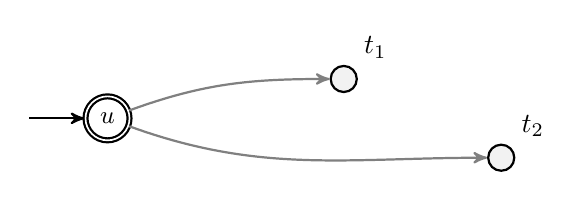
\begin{tikzpicture}[>=stealth', auto, semithick,
        unknown/.style={circle,draw=black,thick,font=\small},
        honest/.style={circle,draw=black,thick,double,font=\small},
        malicious/.style={fill=gray!10,circle,draw=black,thick,font=\small}]
        \node[honest] at (0,0) (u) {$u$};
        \node[malicious] at (3,.5)  (z1) {};
        \node[malicious] at (5,-.5)   (z2) {};
        \path (z1) ++(.4,.4) node {$t_1$};
        \path (z2) ++(.4,.4) node {$t_2$};
        \draw[thick,<-] (u) to (-1,0);
        \draw[thick,<-,gray] (z1) to[out=180,in=20] (u);
        \draw[thick,<-,gray] (z2) to[out=180,in=-20] (u);
      \end{tikzpicture}
    \end{center}
  %  Let $\beta$ denote the smallest honest index of $w$ for which
  %  $\beta \geq \ell(t_2) = \max(\ell(t_1), \ell(t_2))$, with the convention that
  %  $\beta = n+1$ if there is no such index.

    \Paragraph{$\alpha$ must be a uniquely honest slot.}
    We observe, first of all, that the slot $\alpha$ can neither be adversarial nor multihonest:
    otherwise it is easy to construct a fork
    $F^\prime \Fork w$ and a pair of tines in $F^\prime$ that violate~\eqref{eq:tines}. 
    Specifically, construct $F^\prime$ from $F$ by
    adding a new vertex $u^\prime$ to $F$ for which
    $\ell(u^\prime) = \ell(u)$, adding an edge to $u^\prime$ from the
    vertex preceding $u$, and replacing the edge of $t_1$ following $u$
    with one from $u^\prime$; then the other relevant properties of the
    fork are maintained, but the slot divergence of the resulting tines has
    increased by at least one. (See the diagram below.)
    \begin{center}
      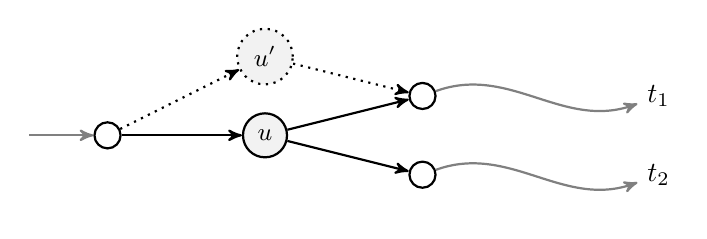
\begin{tikzpicture}[>=stealth', auto, semithick,
        unknown/.style={circle,draw=black,thick,font=\small},
        honest/.style={circle,draw=black,thick,double,font=\small},
        malicious/.style={fill=gray!10,circle,draw=black,thick,font=\small}]
        \node[malicious] at (2,0) (v) {$u$};
        \node[malicious,dotted] at (2,1) (u) {$u^\prime$};
        \node[unknown] at (4,-.5)  (b1) {};
        \node[unknown] at (4,.5)  (a1) {};
        \node[unknown] at (0,0) (base) {};
        \node at (7,.5) (t1) {$t_1$};
        \node at (7,-.5) (t2) {$t_2$};
        % \node[state,honest] at (3,-1) (bottom) {};
        % \node[state,honest] at (7,1) (top) {$H$};
        \draw[thick,->] (base) -- (v);
        \draw[thick,->] (v) -- (a1);
        \draw[thick,->] (v) -- (b1);
        \draw[thick,->,dotted] (u) -- (a1);
        \draw[thick,->,dotted] (base) -- (u);
        \draw[thick,<-,gray] (t1) to[in=20,out=200] (a1);
        \draw[thick,<-,gray] (t2) to[in=20,out=200] (b1);
        \draw[thick,<-,gray] (base) to (-1,0);
        % \draw[thick,<->] (3,0) -- (7,0) node[pos=.5] {$\gap(f)$};
      \end{tikzpicture}
    \end{center}
    
    \Paragraph{$F_x$ has a unique, longest (and honest) tine $t_u$.}
    A similar argument implies that the fork
    $F_x$ has a unique vertex of depth $\depth(u)$: namely, $u$ itself. In
    the presence of another vertex $u^\prime$ (of $F_x$) with depth
    $\depth(u)$, ``redirecting'' $t_1$ through $u^\prime$ (as in the
    argument above) would likewise result in a fork with 
    a larger slot divergence. 
    To see this, notice that $\ell(u^\prime)$ must be strictly less than $\ell(u)$ 
    since $\ell(u)$ is an honest slot (which means $u$ is the only vertex at that slot).
    Thus $\ell(\cdot)$ would indeed be increasing along
    this new tine (resulting from redirecting $t_1$).
    As $\alpha$ is the last index of the string $x$, this additionally
    implies that $F_x$ has no vertices of depth exceeding $\depth(u)$. 
    Let $t_u \in F_x$ be the tine with $\ell(t_u) = \alpha$. 
    \begin{equation}\label{eq:tu}
        \text{The honest tine $t_u$ is the unique longest tine in $F_x$}
        \,.
    \end{equation}
    


    \Paragraph{Identifying $y$.}
    Let $\beta$ denote the smallest honest index of $w$ for which 
    $\beta \geq \ell(t_2)$, with the convention that if there is no such
    index we define $\beta = T + 1$. 
    % If $\ell(t_2)$ is an honest slot 
    % then $\beta = \ell(t_2) \geq \ell(t_1)$.
    % % since slot $\ell(t_2)$ can be associated with a single tine. 
    % % On the other hand, 
    % Otherwise, 
    % % if $\ell(t_2)$ is not an honest slot then 
    % $\beta > \ell(t_2) \geq \ell(t_1)$. 
    % In any case, we conclude that $\beta - 1 \geq \ell(t_1)$. 
    Thus $\beta \geq \ell(t_2) \geq \ell(t_1)$.
    These indices, $\alpha$ and $\beta$, distinguish the
    substrings $y = w_{\alpha+1} \ldots w_{\beta-1}$ and 
    $z = w_{\beta} \ldots w_T$; 
    we will focus on $y$ in the remainder of the proof. 
    Since the function
    $\ell(\cdot)$ is strictly increasing along any tine, observe that
    \begin{align*}
        |y| 
        &= (\beta - 1) - (\alpha + 1) + 1 
        = \beta - \alpha - 1 
        \geq (\ell(t_1) - \ell(u)) - 1 
        \geq (k + 1) - 1 
        = k
        \,.
    \end{align*}
    Hence $y$ has the desired length and it suffices to establish that it is forkable.\footnote{
      In~\citet{LinearConsistency}, $|y|$ was at least $k + 1$. 
      The difference is due to the fact that 
      in their analysis, a slot with multiple vertices 
      was necessarily adversarial. 
    }
    % We can extract from $F$ a balanced fork for $y$ in
    % two steps: First, we subject the fork $F$ to some minor
    % restructuring to ensure that all ``long'' tines pass through $u$. 
    % Next, we construct a fork $\tilde{F}_y$ for $y$ by treating the vertex $u$ as the
    % root of a portion of the subtree of $F$ labeled with the indices of
    % $y$. 
    % The segments of the two tines $t_1$ and $t_2$ in $\tilde{F}_y$ 
    % will yield two maximally long disjoint tines; 
    % thus, $\tilde{F}_y$ will be balanced.

    
    \Paragraph{Honest indices in $xy$ have small depths.}
    The minimality assumption~\eqref{eq:minimality} implies that any honest
    index $h$ for which $h < \beta$ has depth no more than
    $\min(\length(t_1),\length(t_2))$: specifically, we claim that 
    \begin{equation}\label{eq:honest-depth}
      h < \beta \quad\Longrightarrow \quad \hdepth(h) \leq \min(\length(t_1), \length(t_2))\,.
    \end{equation}
    To see this, consider an honest index $h,h < \beta$ and a tine $t_h$
    for which $\ell(t_h) = h$. 
    % Recall that $t_1$ and $t_2$ are viable and 
    If $\ell(t_2)$ is honest then $h < \beta = \ell(t_2)$. 
    Otherwise, $h < \ell(t_2) < \beta$ since $\ell(t_2)$ is adversarial. 
    In any case, $h < \ell(t_2)$ and, 
    since $t_2$ is viable, it follows immediately that
    $\hdepth(h) \leq \length(t_2)$. 
    Similarly, if $h < \ell(t_1)$ 
    then $\hdepth(h) \leq \length(t_1)$ since $t_1$ is viable as well. 
    
    Now consider the case $h = \ell(t_1)$. 
    % \Paragraph{If $\ell(t_1) < \ell(t_2)$, 
    % then $t_1$ is maximally long among all tines with the same label.} 
    We claim that 
    \begin{equation}\label{eq:hdepth-t1}
      \text{
        If $h = \ell(t_1) < \beta$ then $\hdepth(h) = \length(t_1)$ 
        }
      \,.
    \end{equation}
    We can rule out the case $h = \ell(t_1) = \ell(t_2)$ 
    since if this happens, 
    $\ell(t_2)$ is honest and $\beta = \ell(t_2)$, 
    contradicting our assumption that $h < \beta$. 
    Thus, it must be the case that $h = \ell(t_1) < \ell(t_2)$.    
    In this case, the claim follows trivially 
    if $\ell(t_1)$ is a uniquely honest slot. 
    Otherwise, let $t$ be a tine 
    with the maximum length among all tines 
    labeled with the multihonest slot $h = \ell(t_1) < \ell(t_2)$. 
    We wish to show that $\length(t_1) = \length(t)$. 
    There are four contingencies to consider; 
    the first three of these lead to contradictions 
    and for the last one, we get $\length(t_1) = \hdepth(h) = \length(t)$.
    \begin{itemize}

      \item If $(t, t_2) \not \in A$, 
      $\SlotDivergence(t, t_2)$ is at most $k$.
      Since $\SlotDivergence(t_1, t_2)$ is at least $k + 1$, 
      $t$ must share a vertex with $t_2$ after slot $\ell(u)$. 
      But this means $\ell(t \Intersect t_1) = \ell(u)$ 
      and $\SlotDivergence(t, t_1) = \SlotDivergence(t_1, t_2) \geq k + 1$. 
      As a result, $(t, t_1) \in A$. 
      However, this violates~\eqref{eq:minimality} 
      since $|\ell(t) - \ell(t_1)| = 0 < |\ell(t_2) - \ell(t_1)|$ by assumption. 

      \item 
      If $(t, t_2)$ is in $A$ and 
      $\ell(t \Intersect t_1) < \ell(u)$, 
      then $\SlotDivergence(t, t_1) > \SlotDivergence(t_1, t_2)$, 
      violating~\eqref{eq:tines}. 

      \item 
      If $(t, t_2)$ is in $A$ and 
      $\ell(t \Intersect t_1) = \ell(u)$, 
      this means $t$ is disjoint with $t_1$ after $\ell(u)$. 
      Then~\eqref{eq:minimality} is violated 
      since $\SlotDivergence(t, t_1) = \SlotDivergence(t_1, t_2)$ but 
      $|\ell(t) - \ell(t_1)| = 0 < |\ell(t_2) - \ell(t_1)|$ by assumption. 

      \item 
      If $(t, t_2)$ is in $A$ and 
      $\ell(t \Intersect t_1) > \ell(u)$, 
      this means $t$ shares a vertex with $t_1$ after $\ell(u)$. 
      Then $\SlotDivergence(t, t_2) = \SlotDivergence(t_1, t_2)$ 
      and $|\ell(t_2) - \ell(t_1)| = |\ell(t_2) - \ell(t)|$. 
      By~\eqref{eq:length-multihonest}, 
      $\length(t_1) \geq \length(t)$; 
      hence $\length(t_1) = \length(t)$ since by assumption, 
      $t$ has the maximum length among all tines with label $\ell(t_1)$. 
      Hence $\length(t_1) = \hdepth(h)$.

    \end{itemize}
    The remaining case for proving~\eqref{eq:honest-depth}, 
    i.e., when $\ell(t_1) < h < \ell(t_2)$, 
    can be ruled out by the argument below.




    \Paragraph{There is no honest index between $\ell(t_1)$ and $\ell(t_2)$.}
    We claim that 
    \begin{equation}\label{eq:no-honest-index}
        \text{There is no honest index $h$ satisfying $\ell(t_1) < h < \ell(t_2)$}
        \,.
    \end{equation}
    The claim above is trivially true if $\ell(t_1) = \ell(t_2)$.
    Otherwise, suppose (toward a contradiction) 
    that $h$ is an honest index satisfying $\ell(t_1) < h < \ell(t_2)$. 
    Let $t_h$ be an honest tine at slot $h$. 
    The tine-pair $(t_1, t_h)$ may or may not be in $A$. 
    We will show that both cases lead to contradictions.
    \begin{itemize}
      \item If $(t_1, t_h)$ is in $A$ and $\ell(t_1 \Intersect t_h) \leq \ell(u)$, 
      $\SlotDivergence(t_1, t_h)$ is at least $\SlotDivergence(t_1, t_2)$. 
      In fact, due to~\eqref{eq:tines}, this inequality must be an equality. 
      However, the assumption $\ell(t_1) < h < \ell(t_2)$ contradicts~\eqref{eq:minimality}. 

      \item If $(t_1, t_h)$ is in $A$ and $\ell(t_1 \Intersect t_h) > \ell(u)$, 
      it follows that $\SlotDivergence(t_h, t_2) > \SlotDivergence(t_1, t_2)$. 
      As the latter quantity is at least $k + 1$, $(t_h, t_2)$ must be in $A$. 
      The preceding inequality, however, contradicts~\eqref{eq:tines}.

      \item If $(t_1, t_h) \not \in A$, 
      $\SlotDivergence(t_1, t_h)$ is at most $k$.
      As $\SlotDivergence(t_1, t_2)$ is at least $k + 1$, 
      % it follows that $\ell(t_1) - \ell(t_1 \Intersect t_h) > \ell(u)$.
      $t_h$ and $t_1$ must share a vertex after slot $\ell(u)$. 
      Since $\ell(t_1) < h < \ell(t_2)$ by assumption, 
      $\SlotDivergence(t_h, t_2) > \SlotDivergence(t_1, t_2) \geq k + 1$ 
      and, as a result, $(t_h, t_2) \in A$. 
      However, the strict inequality above violates~\eqref{eq:tines}. 
    \end{itemize}
    We conclude that~\eqref{eq:no-honest-index}---and thus~\eqref{eq:honest-depth}---is true. 
    (Note that in the above argument, all we needed was that $t_h$ is a viable tine 
    since in all cases, $t_h$ appears in a tine-pair in $A$. 
    Thus~\eqref{eq:no-honest-index} can be generalized as saying 
    ``there is no fork for $w$ with a viable tine $t$ so that $\ell(t_1) < \ell(t) < \ell(t_2)$.'')
    


  \Paragraph{A fork $\pinch{u}{F}$ where all long tines go through $u$.}
    In light of the remarks above, we observe that the fork $F$ may be
    ``pinched'' at $u$ to yield an essentially identical fork
    $\pinch{u}{F} \vdash w$ with the exception that all tines of length
    exceeding $\depth(u)$ pass through the vertex $u$. Specifically, the
    fork $\pinch{u}{F} \vdash w$ is defined to be the graph obtained
    from $F$ by changing every edge of $F$ directed towards a vertex of
    depth $\depth(u) + 1$ so that it originates from $u$. To see that
    the resulting tree is a well-defined fork, it suffices to check that
    $\ell(\cdot)$ is still increasing along all tines of
    $\pinch{u}{F}$. For this purpose, consider the effect of this
    pinching on an individual tine $t$ terminating at a particular
    vertex $v$---it is replaced with a tine $\pinch{u}{t}$ defined so
    that:
    \begin{itemize}
    \item If $\length(t) \leq \depth(u)$, the tine $t$ is unchanged:
      $\pinch{u}{t} = t$.
    \item Otherwise, $\length(t) > \depth(u)$ and $t$ has a vertex $v$
      of depth $\depth(u) + 1$; note that $\ell(v) > \ell(u)$ because
      $F_x$ contains no vertices of depth exceeding $\depth(u)$. Then
      $\pinch{u}{t}$ is defined to be the path given by the tine
      terminating at $u$, a (new) edge from $u$ to $v$, and the suffix
      of $t$ beginning at $z$. (As $\ell(v) > \ell(u)$ this has the
      increasing label property.)
    \end{itemize}
    Thus the tree $\pinch{u}{F}$ is a legal fork on the same vertex set;
    note that the depths of vertices in $F$ and $\pinch{u}{F}$ are
    identical.
    
    \Paragraph{Constructing a fork $F_y \Fork y$ containing two long tines.}
    By excising the tree rooted at $u$ from this pinched fork
    $\pinch{u}{F}$, we may extract a fork for the string
    $w_{\alpha+1} \dots w_T$. Specifically, consider the induced
    subgraph $\cut{u}{F}$ of $\pinch{u}{F}$ given by the vertices
    $\{u\} \cup \{ v \SuchThat \depth(v) > \depth(u)\}$. By treating $u$ as a
    root vertex and suitably defining the labels $\cut{u}{\ell}$ of
    $\cut{u}{F}$ so that $\cut{u}{\ell}(v) = \ell(v) - \ell(u)$, this
    subgraph has the defining properties of a fork for
    $w_{\alpha+1} \ldots w_T$. In particular, considering that
    $\alpha$ is honest, it follows that each honest index $h > \alpha$
    has depth $\hdepth(h) > \length(u)$ and hence any vertex with label $h$ 
    is also present in $\cut{u}{F}$. 
    For a tine $t$ of $\pinch{u}{F}$, we let $\cut{u}{t}$
    denote the suffix of this tine beginning at $u$, which forms a tine
    in $\cut{u}{F}$. (If $\length(t) \leq \depth(u)$, we define
    $\cut{u}{t}$ to consist solely of the vertex $u$.)  
    Considering $\cut{u}{t_1}$ and $\cut{u}{t_2}$, 
    let $\check{t}_i, i \in \{1, 2\}$ be the longest prefix of $\cut{u}{t_i}$ 
    so that $\check{t}_i$ is labeled by a slot in $y$.
    Since the tines $\cut{u}{t_1}, \cut{u}{t_2}$ are disjoint in $\cut{u}{F}$, 
    so are $\check{t}_1,\check{t}_2$. 
    % Moreover, 
    % since all labels of $\cut{u}{t_1}$ are drawn from
    % $y$, it follows that $\check{t}_1 = \cut{u}{t_1}$. 
    
    Recall that that $y$ is as a prefix of $w_{\alpha+1} \ldots w_T$.
    Let $h^*$ be the largest honest index in $y$. 
    Let $F_y$ denote the subtree of $\cut{u}{F}$, with the same root as $\cut{u}{F}$, 
    containing the following tines: 
    $\check{t}_1, \check{t}_2$, and 
    all tines $\cut{u}{t} \in \cut{u}{F} \setminus \{\check{t}_1, \check{t}_2\}$ so that 
    $\ell(\cut{u}{t})$ is drawn from $y$ and 
    \begin{equation}\label{eq:tines-Fy}
      % \length(\cut{u}{t}) \leq \max_{\substack{h \leq |y|\\ \text{$h$ honest} } } \hdepth(h)
      \length(\cut{u}{t}) \leq \hdepth(h^*)
      \,.
    \end{equation}
    Note that the length of every honest tine 
    labeled by $y$ is at most $\hdepth(h^*)$; 
    hence, thanks to~\eqref{eq:honest-depth}, 
    $F_y$ contains all honest tines from $\cut{u}{F}$ 
    that have labels in $y$. 
    Note, in addition, that the tines $\check{t}_1$ and $\check{t}_2$ 
    are consistently labeled in $F_y$. 
    Thus $F_y$ satisfies all properties of a legal fork. 
    
    Having defined $F_y$, we claim that 
    \begin{equation}\label{eq:two-long-tines}
        \min\left(\length(\check{t}_1), \length(\check{t}_2) \right) \geq \hdepth(h^*)
        % \text{$\check{t}_1$ and $\check{t}_2$ are 
        % maximally long in $F_y \Fork y$}
        \,.
    \end{equation}
    % Considering~\eqref{eq:tines-Fy}, it suffices to show that the length of 
    % $\check{t}_i, i \in \{1,2\}$ is at least $\hdepth(h^*)$. 
    % To see this, first consider $\check{t}_1$. 
    Let $i \in \{1,2\}$.
    If $\ell(t_i) < \beta$ then $\check{t}_i = \cut{u}{t_i}$ and,
    by~\eqref{eq:honest-depth}, $\length(\check{t}_i) = \length(\cut{u}{t_i}) \geq \hdepth(h^*)$. 
    Otherwise, we have $\ell(t_i) = \beta$ which means 
    $\ell(t_i)$ is an honest slot. 
    Thus $\cut{u}{t_i}$ must be an honest tine, 
    building directly on top of the viable tine $\check{t}_i$. 
    Therefore, we have $\length(\check{t}_i) \geq \hdepth(h^*)$.

    % As for $\check{t}_2$,
    % observe that if $\ell(t_2)$ is not honest then $\beta > \ell(t_2)$
    % so that, as with $\check{t}_1$, the tine $\check{t}_2$ is labeled by
    % $y$; a similar argument, relying
    % on~\eqref{eq:honest-depth}, ensures that $\length(\check{t}_2)$ 
    % is at least $\hdepth(h^*)$. 
    % If $\ell(t_2)$ is
    % honest then $\beta = \ell(t_2)$ and the terminal vertex of
    % $\cut{u}{t_2}$ does not appear in $F_y$ since $\ell(\cut{u}{t_2})$ falls outside 
    % $y$. In this case, however,
    % $\length(\cut{u}{t_2}) > \hdepth(h^*)$ for any honest index $h$ of
    % $y$. 
    % It follows that
    % $\length(\check{t}_2)$, which equals $\length(\cut{u}{t_2}) - 1$, 
    % is at least $\hdepth(h^*)$, as desired. 

    \Paragraph{Constructing a balanced fork $\tilde{F}_y \Fork y$.}    
    If $\length(\check{t}_1) = \length(\check{t}_2)$, set $\tilde{F}_y = F_y$ 
    and, due to~\eqref{eq:tines-Fy} and~\eqref{eq:two-long-tines}, 
    the fork $\tilde{F}_y \Fork y$ must be balanced. 
    Otherwise, 
    let $a, b \in \{1, 2\}, a \neq b$ be two integers so that 
    $\length(\check{t}_a) > \length(\check{t}_b)$. 
    We modify $F_y$ by deleting some trailing nodes from $\check{t}_a$ 
    so that the surviving prefix---let it be denoted by $\Final{t}_a$---has the same length as $\check{t}_b$. 
    That is, we achieve 
    \[
      \length(\Final{t}_a) = \length(\check{t}_b) = \min\left(\length(\check{t}_1), \length(\check{t}_2) \right)
      \,. 
    \]
    Let $\tilde{F}_y$ be the resulting fork. 
    Equations~\eqref{eq:tines-Fy} and~\eqref{eq:two-long-tines} imply that 
    $\tilde{F}_y$ has at least two maximum-length tines (i.e., $\Final{t}_a$ and $\check{t}_b$) 
    and therefore, it is balanced.
    It remains to show that the longer tine, $\check{t}_a$, 
    has sufficiently many trailing adversarial vertices so that after deleting them, 
    we obtain 
    $\length(\Final{t}_a) = \length(\check{t}_b)$. 
    (If we had to delete an honest vertex in this process, 
    $\tilde{F}_y$ may have violated 
    property~\ref{fork:unique-honest-mh} in the definition of a fork.)    
    Let $h_a$ be the label of the last honest vertex 
    on $\check{t}_a$. 
    Thanks to~\eqref{eq:two-long-tines}, 
    we have 
    $\length(\check{t}_a) > \length(\check{t}_b) \geq \hdepth(h^*) \geq \hdepth(h_a)$. 
    % and importantly, by~\eqref{eq:no-honest-index}, 
    Hence all vertices in $\check{t}_a$ 
    with labels in $[h_a + 1, \ell(\check{t}_a)]$ 
    must be adversarial; 
    we can safely delete $|\length(\check{t}_a) - \length(\check{t}_b)|$ 
    of these adversarial vertices.

    
    \Paragraph{An $x$-balanced fork $\hat{F} \ForkPrefix F$.} 
    Let us identify the root of the fork $\tilde{F}_y$ with the vertex $u$ of $F_x$ and 
    let $\hat{F}$ be the resulting graph (after ``gluing'' the root of $\tilde{F}_y$ to $u$). 
    By~\eqref{eq:tu}, it is easy to see that the fork 
    $\hat{F} \ForkPrefix F$ 
    is indeed a valid fork on the string $x y$. 
    Moreover, $\hat{F}$ is $x$-balanced since $\tilde{F}_y$ is balanced. 
    The claim in Theorem~\ref{thm:divergence-settlement} follows immediately since $|y| \geq k$.
  
    \hfill$\qed$


  % \end{proof}




\section*{Acknowledgments}
We thank Peter Ga\v{z}i (IOHK) for finding a bug in Fact~\ref{fact:fork-structure} in a previous version of this paper. 


\bibliography{forks,abbrev0,crypto_crossref}

\appendix


% \section{Catalan slots and relative margin}
% \label{sec:fork-margin-catalan}\label{sec:catalan-margin}
% 

In this section, we present the connections between Catalan slots and these elements (namely, the ``relative margin''). 
The exposition culminates in Corollary~\ref{coro:catalan-margin-critical} 
which characterizes a Catalan slot in terms of relative margin. 
This directly connects the consistency analysis in Sleepy~\cite{Sleepy} 
and~\cite{LinearConsistency} through the observations made in this paper.



% 
\subsection{Closed forks, reach, and extensions}
\begin{definition}[Closed fork]
  A fork $F$ is \emph{closed} if every leaf is honest. For convenience, we say the trivial fork is closed.
\end{definition}
Closed forks have two nice properties that make them especially useful in reasoning about the view of honest parties.
First, 
all honest observers will select a unique longest tine from this fork 
(since all longest tines in a closed fork are honest, 
honest parties are aware of all previous honest blocks, 
they observe the longest chain rule, and they employ the same consistent tie-breaking rule).  
Second, 
% recalling our description of the
% settlement game, 
closed forks intuitively capture decision points for the adversary.
The adversary can potentially show many tines to many honest parties, 
but once an honest node has been placed on top of 
a tine, any adversarial blocks beneath it are part of the public record and are visible to all honest parties. 
For these
reasons, we will often find it easier to reason about closed forks than arbitrary forks. % (without loss of generality).

The next few definitions are the start of a general toolkit for reasoning about an adversary's capacity to build highly diverging paths in forks, based on the underlying characteristic string.
%current state of a fork.

%%%%Reach and margin
\begin{definition}[Gap, reserve, and reach]\label{def:gap-reserve-reach-mh}
For a closed fork $F \vdash w$ and its unique longest tine $\hat{t}$, we define the \emph{gap} of a tine $t$ to be $\gap(t)=\length(\hat{t})-\length(t)$.
Furthermore, we define the \emph{reserve} of $t$, denoted $\reserve(t)$, to be the number of adversarial indices in $w$ that appear after the terminating vertex of $t$. More precisely, if $v$ is the last vertex of $t$, then
\[
  \reserve(t)=|\{\ i \mid w_i=1 \ and \ i > \ell(v)\}|\,.
  \]
These quantities together define the \emph{reach} of a tine: $
\reach(t)=\reserve(t)-\gap(t)$.
\end{definition}

The notion of reach can be intuitively understood as a measure of
the resources available to our adversary in the settlement
game. Reserve tracks the number of slots in which the adversary has
the right to issue new blocks.  When reserve exceeds gap (or
equivalently, when reach is nonnegative), such a tine could be
extended---using a sequence of dishonest blocks---until it is as long
as the longest tine. Such a tine could be offered to an honest player
who would prefer it over, e.g., the current longest tine in the
fork. In contrast, a tine with negative reach is too far behind to be
directly useful to the adversary at that time.

\begin{definition}[Maximum reach]
For a closed fork $F\vdash w$, we define $\rho(F)$ to be the largest reach attained by any tine of $F$, i.e., 
\[
\rho(F)=\underset{t}\max \ \reach(t)\,.
\]
Note that $\rho(F)$ is never negative (as the longest tine of any fork always has reach at least 0). We overload this notation to denote the maximum reach over all forks for a given characteristic string: 
\[
\rho(w)=\underset{\substack{F\vdash w\\\text{$F$ closed}}}\max\big[\underset{t}\max \ \reach(t)\big]\,.
\]
\end{definition}

Reach of vertices is always non-increasing as we move down a tine. 
That is, if $B_1, B_2, \ldots$ are vertices on the same tine in the root-to-leaf order, then 
$\reach(B_i) \leq \reach(B_{i+1})$. 
The inequality is strict if $B_{i + 1}$ is honest. 
Consequently, the reach of an adversarial tine is no more than 
the reach of the last honest vertex in that tine. 
In any fork, the reach of a maximum-length tine is always non-negative. 
Hence, an honest tine with the maximum length over all honest tines 
will always have a non-negative reach. 
Thanks to the monotonicity of the honest-depth function $\hdepth(\cdot)$, 
if there are multiple honest tines 
having the (same) maximum length among all honest tines, 
they must have the same label. 
Therefore, if $h$ is the last honest slot in $w$ and 
$t$ a maximum-length honest tine with label $h$,  
then $\reach(t) \geq 0$. 


% {\color{red} Fix this.}
% \begin{fact}\label{fact:fork-structure-reach}
%   Let $w \in \{\h, \H, \A\}^T$ be a characteristic string, 
%   $s \in [T + 1]$ be an integer, 
%   $x \PrefixEq w, |x| = s - 1$. 
%   Let 
%   $F$ be a fork for $w$, 
%   $B$ an honest vertex in $F$, 
%   $h = \ell(B)$, and 
%   $I = [h + 1, s - 1]$.
%   Let $F_x \Fork x$ be a fork prefix of $F$ so that 
%   $F_x$ contains all honest tines from $F$ with labels at most $s - 1$. 
%   The following statements are equivalent: 
%   \begin{enumerate*}[label=(\roman*)]
%     \item \label{fact-reach-part:Aheavy} $I$ is $\Aheavy$; 
%     \item \label{fact-reach-part:viable-adv-ext} 
%       $B$ has an adversarial extension $t, \ell(t) \in I$ so that $t$ is 
%       viable at the onset of slot $s$; and
%     \item \label{fact-reach-part:nonneg-reach} $\reach_{F_x}(B) \geq 0$;
%   \end{enumerate*}      
% \end{fact}
% \begin{proof}
%   The equivalence between items~\ref{fact-reach-part:Aheavy} and~\ref{fact-reach-part:viable-adv-ext} has already been shown in Fact~\ref{fact:fork-structure}. 
%   \begin{description}[font=\normalfont\itshape\space]

%     \item[\ref{fact-reach-part:nonneg-reach} implies~\ref{fact-reach-part:Aheavy}.]
%       By assumption, $\reach_{F_x}(B)  = \reserve_{F_x}(B) - \gap_{F_x}(B) \geq 0$.               
%       Since $\reserve_{F_x}(B) = \#_\A(I)$ and $\gap_{F_x}(B) \geq \#_\h(I) + \#_\H(I)$, 
%       it follows that $\#_\A(I) \geq \#_\h(I) + \#_\H(I)$. 

%     \item[\ref{fact-reach-part:viable-adv-ext} implies~\ref{fact-reach-part:nonneg-reach}.]
%       Since $t$ is an adversarial extension of $B$, 
%       it contains only adversarial vertices from $I$. 
%       By assumption, $t$ is viable at the onset of slot $s$.
%       It follows that $\#_\A(I) \geq \gap_{F_x}(B)$.
%       Since $\reserve_{F_x}(B) = \#_\A(I)$, we have 
%       $\reach_{F_x}(B) = \reserve_{F_x}(B) - \gap_{F_x}(B) \geq 0$.  
      
%   \end{description}            
% \end{proof}






\paragraph{Non-negative reach, $\A$-heaviness, and viable adversarial extensions.}
Let $w \in \{\h, \H, \A\}^T$,   
$s \in [T + 1]$, and 
$F \Fork w_1 \ldots w_{s - 1}$ an arbitrary fork. 
Let $B \in F$ be an honest vertex 
and $t$ a maximum-length tine in $F$.
Consider the following statements: 
\begin{enumerate}[label=(\alph*)]
  \item \label{fact-reach-part:viable-adv-ext} $B$ has an adversarial extension viable at the onset of slot $s$.
  \item \label{fact-reach-part:nonneg-reach} $\reach_{F}(B)$ is non-negative.
  \item \label{fact-reach-part:Aheavy} The interval $I = [\ell(B) + 1, s - 1]$ is $\Aheavy$. 
  \item \label{fact-reach-part:conservative} $\length(t) = \#_\h(I) + \#_\H(I) + \length(B)$.     
\end{enumerate}

\begin{fact}\label{fact:fork-structure-reach}
    ~\ref{fact-reach-part:viable-adv-ext} $\Longrightarrow$
    \ref{fact-reach-part:nonneg-reach} $\Longrightarrow$
    \ref{fact-reach-part:Aheavy}.
    In addition, if we assume~\ref{fact-reach-part:conservative}, then 
    ~\ref{fact-reach-part:Aheavy} $\Longrightarrow$ 
    ~\ref{fact-reach-part:nonneg-reach} $\Longrightarrow$
    ~\ref{fact-reach-part:viable-adv-ext}.
\end{fact}
Fact~\ref{fact:fork-structure-reach} can be seen as 
a refinement of Fact~\ref{fact:fork-structure} 
when $F$ is a closed fork. 
\begin{proof}~
  \begin{description}[font=\normalfont\itshape\space]
    \item[\ref{fact-reach-part:viable-adv-ext} implies~\ref{fact-reach-part:nonneg-reach}.]
      An adversarial extension of $B$ 
      contains only adversarial vertices from $I$. 
      If this extension is viable at the onset of slot $s$, 
      $\#_\A(I)$ must be at least $\gap_{F}(B)$.
      Since $\reserve_{F}(B) = \#_\A(I)$, we have 
      $\reach_{F}(B) = \reserve_{F}(B) - \gap_{F}(B) \geq 0$.  
      
    \item[\ref{fact-reach-part:nonneg-reach} implies~\ref{fact-reach-part:Aheavy}.]
      By assumption, $\reach_{F}(B)  = \reserve_{F}(B) - \gap_{F}(B) \geq 0$.               
      $t$ contains at least $\#_\h(I) + \#_\H(I)$ vertices from 
      the interval $I$; 
      hence, $\gap_{F}(B) \geq \#_\h(I) + \#_\H(I)$. 
      Since $\reserve_{F}(B) = \#_\A(I)$, 
      it follows that $\#_\A(I) \geq \#_\h(I) + \#_\H(I)$. 

    \item[\ref{fact-reach-part:conservative} and~\ref{fact-reach-part:Aheavy} implies~\ref{fact-reach-part:nonneg-reach}.]
      Since $I$ is $\Aheavy$, 
      $\reserve_F(B) = \#_\A(I) \geq \#_\h(I) + \#_\H(I)$. 
      However, since~\ref{fact-reach-part:conservative} holds, 
      the latter quantity equals $\length(t) - \length(B) = \gap_F(B)$. 
      It follows that $\reach_F(B) = \reserve_F(B) - \gap_F(B) \geq 0$. 

    \item[\ref{fact-reach-part:conservative} and~\ref{fact-reach-part:nonneg-reach} implies~\ref{fact-reach-part:viable-adv-ext}.]
      $I$ contains at least $\gap_F(B)$ adversarial slots. 
      We can use these slots augment $B$ 
      into an adversarial tine $t'$ 
      of length at least $\length(t)$. 
      Thus $t'$ will be viable at the onset of slot $s$.
  \end{description}  
\end{proof}


Observe that for any characteristic string $x$, 
one can \emph{extend} (i.e., augment) a closed fork prefix $F \Fork x$ 
into a larger closed fork $F' \Fork x0$ so that $F \ForkPrefix F'$. 
A \emph{conservative extension} is a minimal extension in that 
it consumes the least amount of reserve (cf. Definition~\ref{def:gap-reserve-reach-mh}), 
leaving the remaining reserve to be used in future.
Extensions and, in particular, conservative extensions 
play a critical role in the exposition that follows. 

\begin{definition}[Extensions]\label{def:extension-mh}  
  Let $w \in \{\h, \H, \A\}^*$ be a characteristic string 
  and $F$ a closed fork for $w$. 
  Let $F'$ be a closed fork for $wb, b \in \{\h, \H\}$ 
  so that $F \ForkPrefix F'$. 
  We say that \emph{$F'$ is an extension of $F$} if 
  every honest vertex in $F'$ either belongs to $F$ or has label $|w| + 1$. 
  Let $\sigma \in F'$ be an honest vertex with $\ell(\sigma) = |w| + 1$ 
  and let $s$ be the longest honest prefix of $\sigma$. 
  (Necessarily, $s \in F$.)
  We say that \emph{$\sigma$ is an extension of $s$}. 
  The new tine $\sigma$ is a \emph{conservative extension} if 
  % $\height(F) + 1 = \max_{t \in S} \length(t)$.  
  $\height(F') = \height(F) + 1$.  
\end{definition} 
Since $F'$ is closed, all longest tines in $F'$ are honest and they have label $|w| + 1$.
% , i.e., they belong to $S$ in the above definition.
Let $\hat{t}$ be the unique longest honest tine in $F'$ 
under the consistent longest-chain selection rule 
in Axiom~\ref{axiom:tie-breaking}.
Now consider a tine $\sigma \in S$. 
Since $\sigma$ is honest, 
it follows that 
$\length(\sigma) 
\geq 1 + \height(F) 
= 1 + \length(s) + \gap_F(s)$ 
where $s \in F$ is the longest honst prefix of $\sigma$.
The root-to-leaf path in $F^\prime$ 
that ends at $\sigma$ 
contains at least $\gap_F(s)$ adversarial vertices $u \in F'$ 
so that $\ell(u) \in [\ell(s) + 1, |w|]$ and 
$u \not \in F$. 
If $\sigma$ is a conservative extension, 
the number of such vertices is exactly $\gap_F(s)$. 
% Finally, if $F'$ is a conservative extension, 
% the height of $F'$ is exactly one more than the height of $F$.


\begin{fact}[Extensions and reach]\label{fact:reach-fork-ext-mh}
  Let $b \in \{\h, \H\}$. 
  Let $F \Fork w$ and $F^\prime \Fork wb$ be closed forks so that 
  $F \ForkPrefix F^\prime$ and 
  $F^\prime$ is obtained from $F$ via one or more extensions 
  $\sigma \in F^\prime, \ell(\sigma) = |w| + 1$.
  Then $\reach_{F^\prime}(t) \leq \reach_F(t) - 1$ for every $t \in F$. 
  If all these extensions are conservative, then 
  $\reach_{F^\prime}(t) = \reach_F(t) - 1$ for every $t \in F$. 
  Furthermore, a conservative extension $\sigma$ satisfies 
  $\reach_{F^\prime}(\sigma) = 0$.
\end{fact}
The above fact follows from the claims below.
\begin{claim}\label{claim:nex-mh}
  Let $b \in \{\h, \H\}$. 
  Consider a closed fork $F\vdash w$ and some closed fork $F'\vdash wb$ such that $F\fprefix F'$. 
  If $t \in F$ then 
  $\reach_{F'}(t)\leq \reach_{F}(t) - 1$. 
  The inequality becomes and equality 
  if $F'$ is obtained via 
  conservative extensions from $F$.
\end{claim}
\begin{proof}
  We know that $\reach_{F'}(t)=\reserve_{F'}(t)-\gap_{F'}(t).$ From $F$ to $F'$, the length of the longest tine increases by at least one, and the length of $t$ does not change. 
  It follows that $\gap_{F'}(t) \geq \gap_{F}(t) + 1$. 
  The inequality becomes an equality 
  if $F'$ is obtained from $F$ via only conservative extensions. 
  The reserve of $t$ does not change, because there are no new $\A$s in the characteristic string. Therefore, 
  $
    \reach_{F'}(t)
    =\reserve_{F'}(t)-\gap_{F'}(t)
    \leq \reserve_{F}(t)-\gap_{F}(t) - 1
    =\reach_{F}(t) - 1
  $. 
\end{proof}
\begin{claim}\label{claim:ex-mh}
  Conservative extensions have reach zero.
  % Let $b \in \{\h, \H\}$. 
  % Consider closed forks $F\vdash w, F'\vdash wb$ 
  % such that $F\fprefix F'$. 
  % If a tine $t$ of $F'$ is a conservative extension 
  % then $\reach_{F'}(t)=0$.
\end{claim}
\begin{proof}
  Let $b \in \{\h, \H\}$. 
  Consider closed forks $F\vdash w, F'\vdash wb$ 
  such that $F\fprefix F'$. 
  Let $t \in F'$ be a conservative extension. 
  This means $t$ is honest, $\ell(t) = |w| + 1$, 
  and 
  $t$ is a longest tine in $F'$. 
  The last statement implies $\gap_{F'}(t)=0$. 
  Since $\reserve_{F'}(t)=0$, it follows that 
  $\reach_{F'}(t)=\reserve_{F'}(t)-\gap_{F'}(t) = 0$. 
\end{proof}


\subsection{Relative margin}
\begin{definition}[The $\sim_x$ relations]
  For two tines $t_1$ and $t_2$ of a fork $F$, we write $t_1 \sim t_2$
  when $t_1$ and $t_2$ share an edge; otherwise we write
  $t_1 \nsim t_2$. We generalize this equivalence relation to reflect
  whether tines share an edge over a particular suffix of $w$: for
  $w = xy$ we define $t_1 \sim_x t_2$ if $t_1$ and $t_2$ share an edge
  that terminates at some node labeled with an index in $y$;
  otherwise, we write $t_1 \nsim_x t_2$ (observe that in this case the
  paths share no vertex labeled by a slot associated with $y$).  We
  sometimes call such pairs of tines \emph{disjoint} (or, if
  $t_1 \nsim_x t_2$ for a string $w = xy$, \emph{disjoint over
    $y$}). Note that $\sim$ and $\sim_\varepsilon$ are the same
  relation.
\end{definition}

\begin{definition}[Margin]\label{def:margin}
The \emph{margin} of a fork $F\vdash w$, denoted $\mu(F)$, is defined as 
\begin{equation}\label{eq:margin-absolute}
\mu(F)=\underset{t_1\nsim t_2}\max \bigl(\min\{\reach(t_1),\reach(t_2)\}\bigr)\,,
\end{equation}
where this maximum is extended over all pairs of disjoint tines of
$F$; thus margin reflects the ``second best'' reach obtained over all
disjoint tines. In order to study splits in the chain over particular portions of a
string, we generalize this to define a ``relative'' notion of margin:
If $w = xy$ for two strings $x$ and $y$ and, as above, $F \vdash w$,
we define
\[
  \mu_x(F)=\underset{t_1\nsim_x t_2}\max \bigl(\min\{\reach(t_1),\reach(t_2)\}\bigr)\,.
\]
Note that $\mu_\varepsilon(F) = \mu(F)$.

For convenience, we once again overload this notation to denote the
margin of a string. $\mu(w)$ refers to the maximum value of $\mu(F)$
over all possible closed forks $F$ for a characteristic string $w$:
\[
\mu(w)=\underset{\substack{F\vdash w,\\ \text{$F$ closed}}}\max \, \mu(F)\,.
\]
Likewise, if $w = xy$ for two strings $x$ and $y$ we define
\[
\mu_x(y)=\underset{\substack{F\vdash w,\\ \text{$F$ closed}}} \max \, \mu_x(F)\,.
\]
%(Cf.~\cite{KRDO17}, which defined and studied the ``absolute'' version
%$\mu(\cdot)$ of this quantity of~\eqref{eq:margin-absolute}.)
\end{definition}
Note that, at least informally, 
disjoint tines with large reach are of natural
interest to an adversary who wants to build an $x$-balanced fork, 
since such a fork contains two (partially disjoint) long tines.
It is easy to see that 
if $w = xx'y$ and 
$\mu_{xx'}(y)$ is negative then $\mu_x(x'y)$ is negative as well.

% \begin{fact}\label{fact:neg-margin}
%   Let $w$ be a characteristic string 
%   and let $w = xx'y$ be an arbitrary decomposition. 
%   If $\mu_{xx'}(y) < 0$ then $\mu_x(x'y) < 0$.
% \end{fact}

The theorem below shows how to recursively compute $\mu_x(y)$ 
for a given decomposition $w = xy$.


% \subsection{The relative margin recurrence}
\begin{theorem}\label{thm:relative-margin}
  Let $\varepsilon$ be the empty string 
  and $b \in \{\h, \H\}$. 
  Then $\rho(\varepsilon) = 0$ 
  and, for all nonempty strings $w \in \{\h, \H, \A\}^*$ 
  \begin{equation}
    \rho(w\A) = \rho(w) + 1\,, \qquad\text{and}\qquad
    \rho(wb) = \begin{cases} 0 & \text{if $\rho(w) = 0$,}\\
      \rho(w)-1 & \text{otherwise.}
    \end{cases}
    \label{eq:rho-recursive-mh}
  \end{equation}


  Furthermore, for any strings $x, y \in\{\h, \H, \A\}\text{\emph{*}}$,
  $\mu_x(\varepsilon) =\rho(x)$, 
  \begin{equation}
    \mu_x(y\A)= \mu_x(y)+1\,,\qquad\text{and}\qquad
    \mu_x(yb)= \begin{cases}
      0 & \text{if $\rho(xy) > \mu_x(y)=0$}\,, \\
      0 & \text{if $\rho(xy) = \mu_x(y) = 0$ and $b = \H$}\,, \\
      \mu_x(y)-1 & \text{otherwise.}
    \end{cases}
    \label{eq:mu-relative-recursive-mh}
  \end{equation}

  % Additionally, for every $w \in \{\h, \H, \A\}^*$ 
  % there exists a canonical fork for $w$. 
\end{theorem}
The proof of Theorem~\ref{thm:relative-margin} is given in Section~\ref{sec:margin-proof}. 
Let $w$ be a characteristic string and 
let $m, k \in \NN$ so that $m + k \leq |w|$. 
Let $x \Prefix w, |x| = m-1$ and $xy \PrefixEq w, |xy| \geq m + k$.
If the symbols in $w$ are independent and identically distributed, 
the recursive formulation in~\eqref{eq:mu-relative-recursive-mh} implies an algorithm --- which takes time and space $O(|w|^3)$ --- 
for computing the probability that $\mu_x(y) \geq 0$. 
But this is exactly the probability that slot $m$ is not $k$-settled, 
according to~\eqref{eq:settlement-uvp} 
and Lemma~\ref{lemma:uvp-margin} below. 
In Section~\ref{sec:exact-prob}, 
we describe this algorithm in more detail and 
compile some explicit values for this probability.








% We can define the ``forkability'' of a
% characteristic string in terms of its margin.
% Although this definition is not necessary for our presentation, it
% reflects the terminology of existing literature.

% \begin{definition}[Forkable strings]\label{def:forkable}
%   A charactersitic string $w$ is \emph{forkable} if its margin is non-negative, i.e., $\mu(w) \geq 0$.
%   Equivalently, $w$ is forkable if there is a balanced fork for $w$.
% \end{definition}

\subsection{Catalan slots and relative margin}

  Below, we lay down the connection between Catalan slots 
  and relative margin. 
  



\break
\newpage
\section{CP violations and balanced forks with concurrent honest leaders}
\label{sec:cp-forks}
Balanced forks played a critical role 
in the analysis of~\cite{LinearConsistency}. 
Specifically, a balanced fork was equivalent to a settlement violation in their setting 
and a CP violation would also imply a balanced fork.
In the current analysis, 
we have analyzed settlement and CP violations through 
their connections with the UVP and Catalan slots; 
thus balanced forks are not necessary in our analysis. 
However, it is instructive to see 
whether the statement ``a CP violation implies a balanced fork'' 
still holds in our model 
and, importantly, 
how the existing proof needs to be modified. 

Thus the goal of this section is to prove 
Theorem~\ref{thm:divergence-settlement} below which 
would yield an alternative proof of Theorem~\ref{thm:main-mh-CP} 
without using the Catalan slots.
However, the simplicity of the proof of Theorem~\ref{thm:main-mh-CP} 
in \Section~\ref{sec:cp-proof-via-uvp} 
demonstrates the expressive power of the UVP and Catalan slots 
compared to relative margin and balanced forks.



\Paragraph{A $\kSlotCP$ violation implies a $k$-settlement violation.}
Let $w$ be a characteristic string, written $w = xy$, 
and let $F$ be a fork for $w$. 
Recall that a slot $s = |x| + 1$ is not $k$-settled 
if and only if $F$ contains 
two maximum-length tines that diverge prior to $s$, 
i.e., $F$ is $x$-balanced (see Definition~\ref{def:balanced-fork}).


\begin{definition}[Slot divergence]\label{def:slot-divergence}
  Let $w \in \{\h, \H, \A\}^*$ and let $F$ be a fork for $w$. 
  Define the \emph{slot divergence} of 
  two tines $t_1, t_2 \in F$ 
  as 
  \begin{equation}\label{eq:slot-divergence-tines}
    \SlotDivergence(t_1, t_2) \defeq \ell(t_1) - \ell(t_1 \Intersect t_2)
    \quad\text{where $\ell(t_1) \leq \ell(t_2)$}
    \,.
  \end{equation}
  We can generalize this notion for forks and characteristic strings as follows: 
  $\SlotDivergence(F) \triangleq \max_{t_1, t_2 \in F} \SlotDivergence(t_1, t_2)$ and 
  $\SlotDivergence(w) \triangleq \max_{F \Fork w} \SlotDivergence(F)$. 
\end{definition}

By definition, a $\kSlotCP$ violation 
implies the existence of a fork with a slot divergence at least $k + 1$. 
Theorem~\ref{thm:divergence-settlement} below 
shows that if a fork has a slot divergence at least $k+1$ then 
there is a balanced fork for a prefix of the same characteristic string so that 
two maximum-length tine diverge prior to last $k$ slots. 
Therefore, a $\kSlotCP$ violation implies an $(s,k)$-settlement violation 
for some slot $s$.



 


\begin{theorem}\label{thm:divergence-settlement}
  Let $k, T \in \NN$.  
  Let $w \in \{\h, \H, \A\}^T$ be a characteristic string 
  % which violates $\kSlotCP$. 
  so that $\SlotDivergence(w) \geq k + 1$.
  Then 
  there is a decomposition $w = xyz$ and a fork $\hat{F} \Fork xy$, 
  % where $|y| \geq k + 1$, 
  where $|y| \geq k$, 
  so that 
  $\hat{F}$ is $x$-balanced.
\end{theorem}


\newcommand{\Final}[1]{\tilde{#1}}

% \subsection{Proof of Theorem~\ref{thm:cp-fork}}
% \begin{proof}
  
  Recall that $\ell(t)$ is the slot index of the last vertex of tine
  $t$.  
  Define $A \triangleq \bigcup_{F \Fork w} A_F$ where, for a
  given fork $F \Fork w$, define
  \[
    A_F \triangleq \left\{
      (\tau_1, \tau_2) \SuchThat \parbox{60mm}{       
      $\tau_1, \tau_2$ are two viable tines in the fork $F$, 
      $\ell(\tau_1) \leq \ell(\tau_2)$, and 
      % the pair $(\tau_1, \tau_2)$ is a witness to a $\kSlotCP$ violation
      $\SlotDivergence(\tau_1, \tau_2) \geq k + 1$
      }
     \right\}
     \,.
  \]
  % Define the \emph{slot divergence} of two tines as 
  % $\SlotDivergence(\tau_1, \tau_2) \defeq \ell(\tau_1) - \ell(\tau_1 \Intersect \tau_2)$ 
  % where $\tau_1 \Intersect \tau_2$ denotes the common prefix 
  % of the tines $\tau_1$ and $\tau_2$. 
  % Recalling the definition of a $\kSlotCP$ violation, it is clear that 
  % \begin{equation}\label{eq:divergence}
  %     \SlotDivergence(\tau_1, \tau_2) \geq k + 1 \quad \text{for all } (\tau_1, \tau_2) \in A
  %     \,.
  % \end{equation}
  % For concreteness and simplicity, we assume that the nodes in $F$ 
  % have been suitably labeled so that the following two conditions are met:
  Notice that there must be a tine-pair $(t_1, t_2) \in A$ which satisfies the following two conditions: 
    \begin{equation}\label{eq:tines}
      \SlotDivergence(t_1, t_2) 
      % = \SlotDivergence(w) 
      % = \max_{(\tau_1, \tau_2) \in T} \SlotDivergence(\tau_1, \tau_2) 
      \text{ is maximal over $A$\,,}
      % \text{and}
    \end{equation}
  % and
  \begin{equation}\label{eq:minimality}
    \parbox{0.85\columnwidth}{\centering
    $| \ell(t_2) - \ell(t_1) |$ 
      is minimal among all tine-pairs in $A$ 
      for which~\eqref{eq:tines} holds\,, 
      }
  \end{equation}
  and
  \begin{equation}\label{eq:length-multihonest}
    \parbox{0.85 \columnwidth}{\centering
    For a fixed $t_2$, 
    the tine $t_1$ has the maximum length 
    over all tines $t_1', \ell(t_1') = \ell(t_1)$ \\
    such that $(t_1', t_2)$ 
    satisfies~\eqref{eq:tines} and~\eqref{eq:minimality}\,. 
    }
    % \text{
    % if $(t_1, t_2), (t_1', t_2') \in A$, 
    % satisfy~\eqref{eq:tines} and~\eqref{eq:minimality} 
    % so that $\ell(t_1) = \ell(t_2)$, 
    % then $\length(t_1) \geq \length(t_2')$  
    % }
    % \,.
  \end{equation}
  (Note that $t_1, t_2$ are not uniquely identified.)
  The tines $t_1, t_2$ will play a special role in our proof; 
  let $F$ be a fork containing these tines. 

  Recall given a characteristic string $w \in \{\h, \H, \A\}^*$, 
  a uniquely honest slot contains the symbol $\h$, 
  a multihonest slot contains the symbol $\H$, 
  and an adversarial slot contains the symbol $\A$.
  We call a slot honest if it contains either an $\h$ or an $\H$; 
  otherwise, we call it an adversarial slot. 

  \Paragraph{The prefix $x$, fork $F_x$, and vertex $u$.} 
  Let $u$ denote the last vertex on the tine
  $t_1 \cap t_2$, as shown in the diagram below, and let
  $\alpha \triangleq \ell(u) = \ell(t_1 \cap t_2)$. 
  Let $x \triangleq w_1, \ldots, w_\alpha$ 
  and let $F_x$ be the fork-prefix of $F$ supported on $x$. 
  We will argue that $\alpha$ must be a uniquely honest slot and, 
  in addition, that 
  $F_x$ must contain a unique longest tine $t_u$ terminating 
  at the vertex $u$. 
  We will also identify a substring 
  % $y, |y| \geq k + 1$ 
  $y, |y| \geq k$ 
  such that $w$ can be written as $w = xyz$. 
  Then we will construct a balanced fork $\tilde{F}_y \Fork y$ by 
  modifying the subgraph of $F$ supported on $y$. 
  We will finish the proof by constructing an $x$-balanced fork by 
  suitably appending $\tilde{F}_y$ to $F_x$.
  % and then appealing to Fact~\ref{fact:margin-balance}.
    
  \begin{center}
      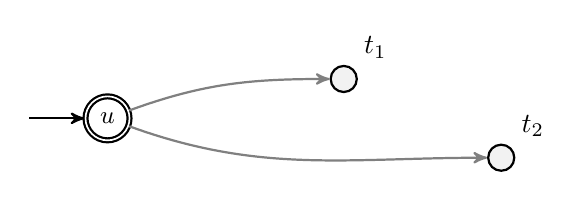
\begin{tikzpicture}[>=stealth', auto, semithick,
        unknown/.style={circle,draw=black,thick,font=\small},
        honest/.style={circle,draw=black,thick,double,font=\small},
        malicious/.style={fill=gray!10,circle,draw=black,thick,font=\small}]
        \node[honest] at (0,0) (u) {$u$};
        \node[malicious] at (3,.5)  (z1) {};
        \node[malicious] at (5,-.5)   (z2) {};
        \path (z1) ++(.4,.4) node {$t_1$};
        \path (z2) ++(.4,.4) node {$t_2$};
        \draw[thick,<-] (u) to (-1,0);
        \draw[thick,<-,gray] (z1) to[out=180,in=20] (u);
        \draw[thick,<-,gray] (z2) to[out=180,in=-20] (u);
      \end{tikzpicture}
    \end{center}
  %  Let $\beta$ denote the smallest honest index of $w$ for which
  %  $\beta \geq \ell(t_2) = \max(\ell(t_1), \ell(t_2))$, with the convention that
  %  $\beta = n+1$ if there is no such index.

    \Paragraph{$\alpha$ must be a uniquely honest slot.}
    We observe, first of all, that the slot $\alpha$ can neither be adversarial nor multihonest:
    otherwise it is easy to construct a fork
    $F^\prime \Fork w$ and a pair of tines in $F^\prime$ that violate~\eqref{eq:tines}. 
    Specifically, construct $F^\prime$ from $F$ by
    adding a new vertex $u^\prime$ to $F$ for which
    $\ell(u^\prime) = \ell(u)$, adding an edge to $u^\prime$ from the
    vertex preceding $u$, and replacing the edge of $t_1$ following $u$
    with one from $u^\prime$; then the other relevant properties of the
    fork are maintained, but the slot divergence of the resulting tines has
    increased by at least one. (See the diagram below.)
    \begin{center}
      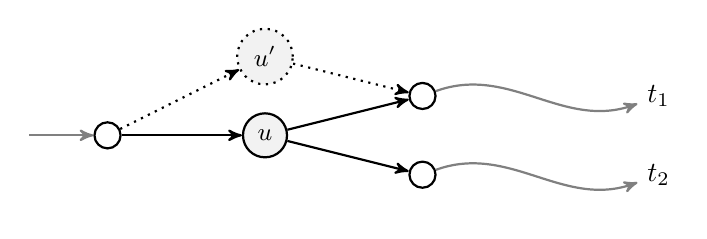
\begin{tikzpicture}[>=stealth', auto, semithick,
        unknown/.style={circle,draw=black,thick,font=\small},
        honest/.style={circle,draw=black,thick,double,font=\small},
        malicious/.style={fill=gray!10,circle,draw=black,thick,font=\small}]
        \node[malicious] at (2,0) (v) {$u$};
        \node[malicious,dotted] at (2,1) (u) {$u^\prime$};
        \node[unknown] at (4,-.5)  (b1) {};
        \node[unknown] at (4,.5)  (a1) {};
        \node[unknown] at (0,0) (base) {};
        \node at (7,.5) (t1) {$t_1$};
        \node at (7,-.5) (t2) {$t_2$};
        % \node[state,honest] at (3,-1) (bottom) {};
        % \node[state,honest] at (7,1) (top) {$H$};
        \draw[thick,->] (base) -- (v);
        \draw[thick,->] (v) -- (a1);
        \draw[thick,->] (v) -- (b1);
        \draw[thick,->,dotted] (u) -- (a1);
        \draw[thick,->,dotted] (base) -- (u);
        \draw[thick,<-,gray] (t1) to[in=20,out=200] (a1);
        \draw[thick,<-,gray] (t2) to[in=20,out=200] (b1);
        \draw[thick,<-,gray] (base) to (-1,0);
        % \draw[thick,<->] (3,0) -- (7,0) node[pos=.5] {$\gap(f)$};
      \end{tikzpicture}
    \end{center}
    
    \Paragraph{$F_x$ has a unique, longest (and honest) tine $t_u$.}
    A similar argument implies that the fork
    $F_x$ has a unique vertex of depth $\depth(u)$: namely, $u$ itself. In
    the presence of another vertex $u^\prime$ (of $F_x$) with depth
    $\depth(u)$, ``redirecting'' $t_1$ through $u^\prime$ (as in the
    argument above) would likewise result in a fork with 
    a larger slot divergence. 
    To see this, notice that $\ell(u^\prime)$ must be strictly less than $\ell(u)$ 
    since $\ell(u)$ is an honest slot (which means $u$ is the only vertex at that slot).
    Thus $\ell(\cdot)$ would indeed be increasing along
    this new tine (resulting from redirecting $t_1$).
    As $\alpha$ is the last index of the string $x$, this additionally
    implies that $F_x$ has no vertices of depth exceeding $\depth(u)$. 
    Let $t_u \in F_x$ be the tine with $\ell(t_u) = \alpha$. 
    \begin{equation}\label{eq:tu}
        \text{The honest tine $t_u$ is the unique longest tine in $F_x$}
        \,.
    \end{equation}
    


    \Paragraph{Identifying $y$.}
    Let $\beta$ denote the smallest honest index of $w$ for which 
    $\beta \geq \ell(t_2)$, with the convention that if there is no such
    index we define $\beta = T + 1$. 
    % If $\ell(t_2)$ is an honest slot 
    % then $\beta = \ell(t_2) \geq \ell(t_1)$.
    % % since slot $\ell(t_2)$ can be associated with a single tine. 
    % % On the other hand, 
    % Otherwise, 
    % % if $\ell(t_2)$ is not an honest slot then 
    % $\beta > \ell(t_2) \geq \ell(t_1)$. 
    % In any case, we conclude that $\beta - 1 \geq \ell(t_1)$. 
    Thus $\beta \geq \ell(t_2) \geq \ell(t_1)$.
    These indices, $\alpha$ and $\beta$, distinguish the
    substrings $y = w_{\alpha+1} \ldots w_{\beta-1}$ and 
    $z = w_{\beta} \ldots w_T$; 
    we will focus on $y$ in the remainder of the proof. 
    Since the function
    $\ell(\cdot)$ is strictly increasing along any tine, observe that
    \begin{align*}
        |y| 
        &= (\beta - 1) - (\alpha + 1) + 1 
        = \beta - \alpha - 1 
        \geq (\ell(t_1) - \ell(u)) - 1 
        \geq (k + 1) - 1 
        = k
        \,.
    \end{align*}
    Hence $y$ has the desired length and it suffices to establish that it is forkable.\footnote{
      In~\citet{LinearConsistency}, $|y|$ was at least $k + 1$. 
      The difference is due to the fact that 
      in their analysis, a slot with multiple vertices 
      was necessarily adversarial. 
    }
    % We can extract from $F$ a balanced fork for $y$ in
    % two steps: First, we subject the fork $F$ to some minor
    % restructuring to ensure that all ``long'' tines pass through $u$. 
    % Next, we construct a fork $\tilde{F}_y$ for $y$ by treating the vertex $u$ as the
    % root of a portion of the subtree of $F$ labeled with the indices of
    % $y$. 
    % The segments of the two tines $t_1$ and $t_2$ in $\tilde{F}_y$ 
    % will yield two maximally long disjoint tines; 
    % thus, $\tilde{F}_y$ will be balanced.

    
    \Paragraph{Honest indices in $xy$ have small depths.}
    The minimality assumption~\eqref{eq:minimality} implies that any honest
    index $h$ for which $h < \beta$ has depth no more than
    $\min(\length(t_1),\length(t_2))$: specifically, we claim that 
    \begin{equation}\label{eq:honest-depth}
      h < \beta \quad\Longrightarrow \quad \hdepth(h) \leq \min(\length(t_1), \length(t_2))\,.
    \end{equation}
    To see this, consider an honest index $h,h < \beta$ and a tine $t_h$
    for which $\ell(t_h) = h$. 
    % Recall that $t_1$ and $t_2$ are viable and 
    If $\ell(t_2)$ is honest then $h < \beta = \ell(t_2)$. 
    Otherwise, $h < \ell(t_2) < \beta$ since $\ell(t_2)$ is adversarial. 
    In any case, $h < \ell(t_2)$ and, 
    since $t_2$ is viable, it follows immediately that
    $\hdepth(h) \leq \length(t_2)$. 
    Similarly, if $h < \ell(t_1)$ 
    then $\hdepth(h) \leq \length(t_1)$ since $t_1$ is viable as well. 
    
    Now consider the case $h = \ell(t_1)$. 
    % \Paragraph{If $\ell(t_1) < \ell(t_2)$, 
    % then $t_1$ is maximally long among all tines with the same label.} 
    We claim that 
    \begin{equation}\label{eq:hdepth-t1}
      \text{
        If $h = \ell(t_1) < \beta$ then $\hdepth(h) = \length(t_1)$ 
        }
      \,.
    \end{equation}
    We can rule out the case $h = \ell(t_1) = \ell(t_2)$ 
    since if this happens, 
    $\ell(t_2)$ is honest and $\beta = \ell(t_2)$, 
    contradicting our assumption that $h < \beta$. 
    Thus, it must be the case that $h = \ell(t_1) < \ell(t_2)$.    
    In this case, the claim follows trivially 
    if $\ell(t_1)$ is a uniquely honest slot. 
    Otherwise, let $t$ be a tine 
    with the maximum length among all tines 
    labeled with the multihonest slot $h = \ell(t_1) < \ell(t_2)$. 
    We wish to show that $\length(t_1) = \length(t)$. 
    There are four contingencies to consider; 
    the first three of these lead to contradictions 
    and for the last one, we get $\length(t_1) = \hdepth(h) = \length(t)$.
    \begin{itemize}

      \item If $(t, t_2) \not \in A$, 
      $\SlotDivergence(t, t_2)$ is at most $k$.
      Since $\SlotDivergence(t_1, t_2)$ is at least $k + 1$, 
      $t$ must share a vertex with $t_2$ after slot $\ell(u)$. 
      But this means $\ell(t \Intersect t_1) = \ell(u)$ 
      and $\SlotDivergence(t, t_1) = \SlotDivergence(t_1, t_2) \geq k + 1$. 
      As a result, $(t, t_1) \in A$. 
      However, this violates~\eqref{eq:minimality} 
      since $|\ell(t) - \ell(t_1)| = 0 < |\ell(t_2) - \ell(t_1)|$ by assumption. 

      \item 
      If $(t, t_2)$ is in $A$ and 
      $\ell(t \Intersect t_1) < \ell(u)$, 
      then $\SlotDivergence(t, t_1) > \SlotDivergence(t_1, t_2)$, 
      violating~\eqref{eq:tines}. 

      \item 
      If $(t, t_2)$ is in $A$ and 
      $\ell(t \Intersect t_1) = \ell(u)$, 
      this means $t$ is disjoint with $t_1$ after $\ell(u)$. 
      Then~\eqref{eq:minimality} is violated 
      since $\SlotDivergence(t, t_1) = \SlotDivergence(t_1, t_2)$ but 
      $|\ell(t) - \ell(t_1)| = 0 < |\ell(t_2) - \ell(t_1)|$ by assumption. 

      \item 
      If $(t, t_2)$ is in $A$ and 
      $\ell(t \Intersect t_1) > \ell(u)$, 
      this means $t$ shares a vertex with $t_1$ after $\ell(u)$. 
      Then $\SlotDivergence(t, t_2) = \SlotDivergence(t_1, t_2)$ 
      and $|\ell(t_2) - \ell(t_1)| = |\ell(t_2) - \ell(t)|$. 
      By~\eqref{eq:length-multihonest}, 
      $\length(t_1) \geq \length(t)$; 
      hence $\length(t_1) = \length(t)$ since by assumption, 
      $t$ has the maximum length among all tines with label $\ell(t_1)$. 
      Hence $\length(t_1) = \hdepth(h)$.

    \end{itemize}
    The remaining case for proving~\eqref{eq:honest-depth}, 
    i.e., when $\ell(t_1) < h < \ell(t_2)$, 
    can be ruled out by the argument below.




    \Paragraph{There is no honest index between $\ell(t_1)$ and $\ell(t_2)$.}
    We claim that 
    \begin{equation}\label{eq:no-honest-index}
        \text{There is no honest index $h$ satisfying $\ell(t_1) < h < \ell(t_2)$}
        \,.
    \end{equation}
    The claim above is trivially true if $\ell(t_1) = \ell(t_2)$.
    Otherwise, suppose (toward a contradiction) 
    that $h$ is an honest index satisfying $\ell(t_1) < h < \ell(t_2)$. 
    Let $t_h$ be an honest tine at slot $h$. 
    The tine-pair $(t_1, t_h)$ may or may not be in $A$. 
    We will show that both cases lead to contradictions.
    \begin{itemize}
      \item If $(t_1, t_h)$ is in $A$ and $\ell(t_1 \Intersect t_h) \leq \ell(u)$, 
      $\SlotDivergence(t_1, t_h)$ is at least $\SlotDivergence(t_1, t_2)$. 
      In fact, due to~\eqref{eq:tines}, this inequality must be an equality. 
      However, the assumption $\ell(t_1) < h < \ell(t_2)$ contradicts~\eqref{eq:minimality}. 

      \item If $(t_1, t_h)$ is in $A$ and $\ell(t_1 \Intersect t_h) > \ell(u)$, 
      it follows that $\SlotDivergence(t_h, t_2) > \SlotDivergence(t_1, t_2)$. 
      As the latter quantity is at least $k + 1$, $(t_h, t_2)$ must be in $A$. 
      The preceding inequality, however, contradicts~\eqref{eq:tines}.

      \item If $(t_1, t_h) \not \in A$, 
      $\SlotDivergence(t_1, t_h)$ is at most $k$.
      As $\SlotDivergence(t_1, t_2)$ is at least $k + 1$, 
      % it follows that $\ell(t_1) - \ell(t_1 \Intersect t_h) > \ell(u)$.
      $t_h$ and $t_1$ must share a vertex after slot $\ell(u)$. 
      Since $\ell(t_1) < h < \ell(t_2)$ by assumption, 
      $\SlotDivergence(t_h, t_2) > \SlotDivergence(t_1, t_2) \geq k + 1$ 
      and, as a result, $(t_h, t_2) \in A$. 
      However, the strict inequality above violates~\eqref{eq:tines}. 
    \end{itemize}
    We conclude that~\eqref{eq:no-honest-index}---and thus~\eqref{eq:honest-depth}---is true. 
    (Note that in the above argument, all we needed was that $t_h$ is a viable tine 
    since in all cases, $t_h$ appears in a tine-pair in $A$. 
    Thus~\eqref{eq:no-honest-index} can be generalized as saying 
    ``there is no fork for $w$ with a viable tine $t$ so that $\ell(t_1) < \ell(t) < \ell(t_2)$.'')
    


  \Paragraph{A fork $\pinch{u}{F}$ where all long tines go through $u$.}
    In light of the remarks above, we observe that the fork $F$ may be
    ``pinched'' at $u$ to yield an essentially identical fork
    $\pinch{u}{F} \vdash w$ with the exception that all tines of length
    exceeding $\depth(u)$ pass through the vertex $u$. Specifically, the
    fork $\pinch{u}{F} \vdash w$ is defined to be the graph obtained
    from $F$ by changing every edge of $F$ directed towards a vertex of
    depth $\depth(u) + 1$ so that it originates from $u$. To see that
    the resulting tree is a well-defined fork, it suffices to check that
    $\ell(\cdot)$ is still increasing along all tines of
    $\pinch{u}{F}$. For this purpose, consider the effect of this
    pinching on an individual tine $t$ terminating at a particular
    vertex $v$---it is replaced with a tine $\pinch{u}{t}$ defined so
    that:
    \begin{itemize}
    \item If $\length(t) \leq \depth(u)$, the tine $t$ is unchanged:
      $\pinch{u}{t} = t$.
    \item Otherwise, $\length(t) > \depth(u)$ and $t$ has a vertex $v$
      of depth $\depth(u) + 1$; note that $\ell(v) > \ell(u)$ because
      $F_x$ contains no vertices of depth exceeding $\depth(u)$. Then
      $\pinch{u}{t}$ is defined to be the path given by the tine
      terminating at $u$, a (new) edge from $u$ to $v$, and the suffix
      of $t$ beginning at $z$. (As $\ell(v) > \ell(u)$ this has the
      increasing label property.)
    \end{itemize}
    Thus the tree $\pinch{u}{F}$ is a legal fork on the same vertex set;
    note that the depths of vertices in $F$ and $\pinch{u}{F}$ are
    identical.
    
    \Paragraph{Constructing a fork $F_y \Fork y$ containing two long tines.}
    By excising the tree rooted at $u$ from this pinched fork
    $\pinch{u}{F}$, we may extract a fork for the string
    $w_{\alpha+1} \dots w_T$. Specifically, consider the induced
    subgraph $\cut{u}{F}$ of $\pinch{u}{F}$ given by the vertices
    $\{u\} \cup \{ v \SuchThat \depth(v) > \depth(u)\}$. By treating $u$ as a
    root vertex and suitably defining the labels $\cut{u}{\ell}$ of
    $\cut{u}{F}$ so that $\cut{u}{\ell}(v) = \ell(v) - \ell(u)$, this
    subgraph has the defining properties of a fork for
    $w_{\alpha+1} \ldots w_T$. In particular, considering that
    $\alpha$ is honest, it follows that each honest index $h > \alpha$
    has depth $\hdepth(h) > \length(u)$ and hence any vertex with label $h$ 
    is also present in $\cut{u}{F}$. 
    For a tine $t$ of $\pinch{u}{F}$, we let $\cut{u}{t}$
    denote the suffix of this tine beginning at $u$, which forms a tine
    in $\cut{u}{F}$. (If $\length(t) \leq \depth(u)$, we define
    $\cut{u}{t}$ to consist solely of the vertex $u$.)  
    Considering $\cut{u}{t_1}$ and $\cut{u}{t_2}$, 
    let $\check{t}_i, i \in \{1, 2\}$ be the longest prefix of $\cut{u}{t_i}$ 
    so that $\check{t}_i$ is labeled by a slot in $y$.
    Since the tines $\cut{u}{t_1}, \cut{u}{t_2}$ are disjoint in $\cut{u}{F}$, 
    so are $\check{t}_1,\check{t}_2$. 
    % Moreover, 
    % since all labels of $\cut{u}{t_1}$ are drawn from
    % $y$, it follows that $\check{t}_1 = \cut{u}{t_1}$. 
    
    Recall that that $y$ is as a prefix of $w_{\alpha+1} \ldots w_T$.
    Let $h^*$ be the largest honest index in $y$. 
    Let $F_y$ denote the subtree of $\cut{u}{F}$, with the same root as $\cut{u}{F}$, 
    containing the following tines: 
    $\check{t}_1, \check{t}_2$, and 
    all tines $\cut{u}{t} \in \cut{u}{F} \setminus \{\check{t}_1, \check{t}_2\}$ so that 
    $\ell(\cut{u}{t})$ is drawn from $y$ and 
    \begin{equation}\label{eq:tines-Fy}
      % \length(\cut{u}{t}) \leq \max_{\substack{h \leq |y|\\ \text{$h$ honest} } } \hdepth(h)
      \length(\cut{u}{t}) \leq \hdepth(h^*)
      \,.
    \end{equation}
    Note that the length of every honest tine 
    labeled by $y$ is at most $\hdepth(h^*)$; 
    hence, thanks to~\eqref{eq:honest-depth}, 
    $F_y$ contains all honest tines from $\cut{u}{F}$ 
    that have labels in $y$. 
    Note, in addition, that the tines $\check{t}_1$ and $\check{t}_2$ 
    are consistently labeled in $F_y$. 
    Thus $F_y$ satisfies all properties of a legal fork. 
    
    Having defined $F_y$, we claim that 
    \begin{equation}\label{eq:two-long-tines}
        \min\left(\length(\check{t}_1), \length(\check{t}_2) \right) \geq \hdepth(h^*)
        % \text{$\check{t}_1$ and $\check{t}_2$ are 
        % maximally long in $F_y \Fork y$}
        \,.
    \end{equation}
    % Considering~\eqref{eq:tines-Fy}, it suffices to show that the length of 
    % $\check{t}_i, i \in \{1,2\}$ is at least $\hdepth(h^*)$. 
    % To see this, first consider $\check{t}_1$. 
    Let $i \in \{1,2\}$.
    If $\ell(t_i) < \beta$ then $\check{t}_i = \cut{u}{t_i}$ and,
    by~\eqref{eq:honest-depth}, $\length(\check{t}_i) = \length(\cut{u}{t_i}) \geq \hdepth(h^*)$. 
    Otherwise, we have $\ell(t_i) = \beta$ which means 
    $\ell(t_i)$ is an honest slot. 
    Thus $\cut{u}{t_i}$ must be an honest tine, 
    building directly on top of the viable tine $\check{t}_i$. 
    Therefore, we have $\length(\check{t}_i) \geq \hdepth(h^*)$.

    % As for $\check{t}_2$,
    % observe that if $\ell(t_2)$ is not honest then $\beta > \ell(t_2)$
    % so that, as with $\check{t}_1$, the tine $\check{t}_2$ is labeled by
    % $y$; a similar argument, relying
    % on~\eqref{eq:honest-depth}, ensures that $\length(\check{t}_2)$ 
    % is at least $\hdepth(h^*)$. 
    % If $\ell(t_2)$ is
    % honest then $\beta = \ell(t_2)$ and the terminal vertex of
    % $\cut{u}{t_2}$ does not appear in $F_y$ since $\ell(\cut{u}{t_2})$ falls outside 
    % $y$. In this case, however,
    % $\length(\cut{u}{t_2}) > \hdepth(h^*)$ for any honest index $h$ of
    % $y$. 
    % It follows that
    % $\length(\check{t}_2)$, which equals $\length(\cut{u}{t_2}) - 1$, 
    % is at least $\hdepth(h^*)$, as desired. 

    \Paragraph{Constructing a balanced fork $\tilde{F}_y \Fork y$.}    
    If $\length(\check{t}_1) = \length(\check{t}_2)$, set $\tilde{F}_y = F_y$ 
    and, due to~\eqref{eq:tines-Fy} and~\eqref{eq:two-long-tines}, 
    the fork $\tilde{F}_y \Fork y$ must be balanced. 
    Otherwise, 
    let $a, b \in \{1, 2\}, a \neq b$ be two integers so that 
    $\length(\check{t}_a) > \length(\check{t}_b)$. 
    We modify $F_y$ by deleting some trailing nodes from $\check{t}_a$ 
    so that the surviving prefix---let it be denoted by $\Final{t}_a$---has the same length as $\check{t}_b$. 
    That is, we achieve 
    \[
      \length(\Final{t}_a) = \length(\check{t}_b) = \min\left(\length(\check{t}_1), \length(\check{t}_2) \right)
      \,. 
    \]
    Let $\tilde{F}_y$ be the resulting fork. 
    Equations~\eqref{eq:tines-Fy} and~\eqref{eq:two-long-tines} imply that 
    $\tilde{F}_y$ has at least two maximum-length tines (i.e., $\Final{t}_a$ and $\check{t}_b$) 
    and therefore, it is balanced.
    It remains to show that the longer tine, $\check{t}_a$, 
    has sufficiently many trailing adversarial vertices so that after deleting them, 
    we obtain 
    $\length(\Final{t}_a) = \length(\check{t}_b)$. 
    (If we had to delete an honest vertex in this process, 
    $\tilde{F}_y$ may have violated 
    property~\ref{fork:unique-honest-mh} in the definition of a fork.)    
    Let $h_a$ be the label of the last honest vertex 
    on $\check{t}_a$. 
    Thanks to~\eqref{eq:two-long-tines}, 
    we have 
    $\length(\check{t}_a) > \length(\check{t}_b) \geq \hdepth(h^*) \geq \hdepth(h_a)$. 
    % and importantly, by~\eqref{eq:no-honest-index}, 
    Hence all vertices in $\check{t}_a$ 
    with labels in $[h_a + 1, \ell(\check{t}_a)]$ 
    must be adversarial; 
    we can safely delete $|\length(\check{t}_a) - \length(\check{t}_b)|$ 
    of these adversarial vertices.

    
    \Paragraph{An $x$-balanced fork $\hat{F} \ForkPrefix F$.} 
    Let us identify the root of the fork $\tilde{F}_y$ with the vertex $u$ of $F_x$ and 
    let $\hat{F}$ be the resulting graph (after ``gluing'' the root of $\tilde{F}_y$ to $u$). 
    By~\eqref{eq:tu}, it is easy to see that the fork 
    $\hat{F} \ForkPrefix F$ 
    is indeed a valid fork on the string $x y$. 
    Moreover, $\hat{F}$ is $x$-balanced since $\tilde{F}_y$ is balanced. 
    The claim in Theorem~\ref{thm:divergence-settlement} follows immediately since $|y| \geq k$.
  
    \hfill$\qed$


  % \end{proof}






% \section{Figures}\label{sec:figures}
% \begin{figure}[t]
  \centering
  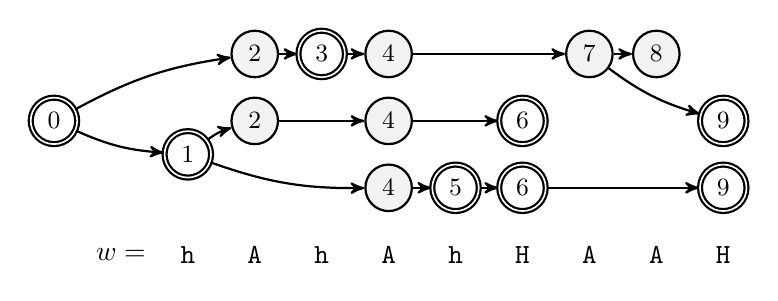
\begin{tikzpicture}[scale=0.85,>=stealth', auto, semithick,
    honest/.style={circle,draw=black,thick,text=black,double,font=\small},
    malicious/.style={fill=gray!10,circle,draw=black,thick,text=black,font=\small}]
    \node at (0,-2) {$w =$};
    \node at (1,-2) {$\h$};
    \node[honest]    at (1,-.5)  (ab1) {$1$};
    \node at (2,-2) {$\A$};
    \node[malicious] at (2,0)  (b2) {$2$}; \node[malicious] at (2,1) (c1) {$2$};
    \node at (3,-2) {$\h$};    \node[honest]    at (3,1)  (c2) {$3$};
    \node at (4,-2) {$\A$};    \node[malicious] at (4,0)  (b3) {$4$}; \node[malicious] at (4,-1) (a2) {$4$};
    \node[malicious] at (4,1) (c3) {$4$};
    \node at (5,-2) {$\h$};    \node[honest]    at (5,-1) (a3) {$5$};
    \node at (6,-2) {$\H$};    \node[honest]    at (6,0)  (b4) {$6$}; \node[honest]    at (6,-1)  (a4) {$6$};
    \node at (7,-2) {$\A$};    \node[malicious] at (7,1)  (c4) {$7$};
    \node at (8,-2) {$\A$};    \node[malicious] at (8,1)  (c5) {$8$};
    \node at (9,-2) {$\H$};    \node[honest]    at (9,0)  (b5) {$9$}; \node[honest]    at (9,-1)  (a5) {$9$};
    \node[honest] at (-1,0) (base) {$0$};
    % \node[state,honest] at (3,-1) (bottom) {};
    % \node[state,honest] at (7,1) (top) {$H$};
    \draw[thick,->] (base) to[bend left=10] (c1);
    \draw[thick,->] (base) to[bend right=10] (ab1);
    \draw[thick,->] (ab1) to[bend right=10] (a2);
    \draw[thick,->] (a2) -- (a3);
    \draw[thick,->] (a3) -- (a4);
    \draw[thick,->] (ab1) to[bend left=10] (b2);
    \draw[thick,->] (b2) -- (b3);
    \draw[thick,->] (b3) -- (b4);
      % \draw[thick,->] (b4) -- (b5);
    \draw[thick,->] (c4) to[bend right=10] (b5);
    \draw[thick,->] (a4) -- (a5);
    \draw[thick,->] (c1) -- (c2);
    \draw[thick,->] (c2) -- (c3);
    \draw[thick,->] (c3) -- (c4);
    \draw[thick,->] (c4) -- (c5);
    % \draw[thick,<->] (3,0) -- (7,0) node[pos=.5] {$\gap(f)$};
  \end{tikzpicture}
  \caption{A fork $F$ for the characteristic string $w = \h\A\h\A\h\H\A\A\H$;
    vertices appear with their labels and honest vertices are
    highlighted with double borders. Note that the depths of the
    (honest) vertices associated with the honest indices of $w$ are
    strictly increasing. Note, also, that this fork has three disjoint
    paths of maximum depth. 
    In addition, two honest vertices have label 6 and two more have label 9, 
    indicating the fact that two honest leaders are associated with each of the (honest) slots 6 and 9. 
    Honest vertices with the same label are concurrent and, therefore, cannot extend each other.
    Note that the two honest vertices with label 6 extend different vertices with the same depth. 
    This is allowed since any tie in the longest-chain rule is broken by the adversary. 
    }
  \label{fig:fork}
\end{figure}





% \section{IEEE}
% \input{ieee_blob}

\end{document}
